\documentclass[twoside]{book}

% Packages required by doxygen
\usepackage{calc}
\usepackage{doxygen}
\usepackage{graphicx}
\usepackage[utf8]{inputenc}
\usepackage{makeidx}
\usepackage{multicol}
\usepackage{multirow}
\usepackage{textcomp}
\usepackage[table]{xcolor}

% Font selection
\usepackage[T1]{fontenc}
\usepackage{mathptmx}
\usepackage[scaled=.90]{helvet}
\usepackage{courier}
\usepackage{amssymb}
\usepackage{sectsty}
\renewcommand{\familydefault}{\sfdefault}
\allsectionsfont{%
  \fontseries{bc}\selectfont%
  \color{darkgray}%
}
\renewcommand{\DoxyLabelFont}{%
  \fontseries{bc}\selectfont%
  \color{darkgray}%
}

% Page & text layout
\usepackage{geometry}
\geometry{%
  a4paper,%
  top=2.5cm,%
  bottom=2.5cm,%
  left=2.5cm,%
  right=2.5cm%
}
\tolerance=750
\hfuzz=15pt
\hbadness=750
\setlength{\emergencystretch}{15pt}
\setlength{\parindent}{0cm}
\setlength{\parskip}{0.2cm}
\makeatletter
\renewcommand{\paragraph}{%
  \@startsection{paragraph}{4}{0ex}{-1.0ex}{1.0ex}{%
    \normalfont\normalsize\bfseries\SS@parafont%
  }%
}
\renewcommand{\subparagraph}{%
  \@startsection{subparagraph}{5}{0ex}{-1.0ex}{1.0ex}{%
    \normalfont\normalsize\bfseries\SS@subparafont%
  }%
}
\makeatother

% Headers & footers
\usepackage{fancyhdr}
\pagestyle{fancyplain}
\fancyhead[LE]{\fancyplain{}{\bfseries\thepage}}
\fancyhead[CE]{\fancyplain{}{}}
\fancyhead[RE]{\fancyplain{}{\bfseries\leftmark}}
\fancyhead[LO]{\fancyplain{}{\bfseries\rightmark}}
\fancyhead[CO]{\fancyplain{}{}}
\fancyhead[RO]{\fancyplain{}{\bfseries\thepage}}
\fancyfoot[LE]{\fancyplain{}{}}
\fancyfoot[CE]{\fancyplain{}{}}
\fancyfoot[RE]{\fancyplain{}{\bfseries\scriptsize Generated on Sun Sep 29 2013 01\-:57\-:08 for Road\-Runner by Doxygen }}
\fancyfoot[LO]{\fancyplain{}{\bfseries\scriptsize Generated on Sun Sep 29 2013 01\-:57\-:08 for Road\-Runner by Doxygen }}
\fancyfoot[CO]{\fancyplain{}{}}
\fancyfoot[RO]{\fancyplain{}{}}
\renewcommand{\footrulewidth}{0.4pt}
\renewcommand{\chaptermark}[1]{%
  \markboth{#1}{}%
}
\renewcommand{\sectionmark}[1]{%
  \markright{\thesection\ #1}%
}

% Indices & bibliography
\usepackage{natbib}
\usepackage[titles]{tocloft}
\setcounter{tocdepth}{3}
\setcounter{secnumdepth}{5}
\makeindex

% Hyperlinks (required, but should be loaded last)
\usepackage{ifpdf}
\ifpdf
  \usepackage[pdftex,pagebackref=true]{hyperref}
\else
  \usepackage[ps2pdf,pagebackref=true]{hyperref}
\fi
\hypersetup{%
  colorlinks=true,%
  linkcolor=blue,%
  citecolor=blue,%
  unicode%
}

% Custom commands
\newcommand{\clearemptydoublepage}{%
  \newpage{\pagestyle{empty}\cleardoublepage}%
}


%===== C O N T E N T S =====

\begin{document}

% Titlepage & ToC
\hypersetup{pageanchor=false}
\pagenumbering{roman}
\begin{titlepage}
\vspace*{7cm}
\begin{center}%
{\Large Road\-Runner }\\
\vspace*{1cm}
{\large Generated by Doxygen 1.8.5}\\
\vspace*{0.5cm}
{\small Sun Sep 29 2013 01:57:08}\\
\end{center}
\end{titlepage}
\clearemptydoublepage
\tableofcontents
\clearemptydoublepage
\pagenumbering{arabic}
\hypersetup{pageanchor=true}

%--- Begin generated contents ---
\chapter{Road\-Runner C++ Library}
\label{index}\hypertarget{index}{}\hypertarget{index_intro_sec}{}\section{\-Introduction}\label{index_intro_sec}
\-Road\-Runner is a \-S\-B\-M\-L compliant high performance and portable simulation engine for systems and synthetic biology. \-To run a simple \-S\-B\-M\-L model and generate time series data we would call\-:


\begin{DoxyCode}
 RRResultHandle result;

 if (!loadSBMLFromFile ("mymodel.xml"))
    exit;

 result = simulate (0, 10, 100);
 printf (resultToString (output)
\end{DoxyCode}


\-More complex example\-:


\begin{DoxyCode}
 #include <stdlib.h>
 #include <stdio.h>
 #include "rr_c_api.h"

 int main(int nargs, char** argv)
 {
        RRHandle rrInstance = getRRInstance();

        printf("loading model file %s\n", argv[1]);
 
        if (!loadSBMLFromFile(argv[1])) {
           printf ("Error while loading SBML file\n");
           printf ("Error message: %s\n", getLastError());
           exit();
        }
                   
        RRResultHandle output = simulate (0, 100, 1000);  // start time, end
       time, and number of points
        
        printf("Output table has %i rows and %i columns\n", output->RSize, 
      output->RCols);
        printResult (output);

        freeResult (output);
        freeRRInstance (rrInstance)

        return 0;
 }
\end{DoxyCode}
 \hypertarget{index_install_sec}{}\section{\-Installation}\label{index_install_sec}
\-Installation documentation is provided in the main google code page. 
\chapter{Deprecated List}
\label{deprecated}
\hypertarget{deprecated}{}

\begin{DoxyRefList}
\item[\label{deprecated__deprecated000002}%
\hypertarget{deprecated__deprecated000002}{}%
Member \hyperlink{classrr_1_1_road_runner_a57f1463dafcc61a90c3122a8fb37b08d}{rr\-:\-:Road\-Runner\-:\-:change\-Initial\-Conditions} (const std\-::vector$<$ double $>$ \&ic)]
\item[\label{deprecated__deprecated000005}%
\hypertarget{deprecated__deprecated000005}{}%
Member \hyperlink{classrr_1_1_road_runner_acb6ac6676114cf7658d39af85f19b0d3}{rr\-:\-:Road\-Runner\-:\-:get\-Available\-Time\-Course\-Symbols} ()]
\item[\label{deprecated__deprecated000017}%
\hypertarget{deprecated__deprecated000017}{}%
Member \hyperlink{classrr_1_1_road_runner_afc7498e1fe7098233c87f4427e74509b}{rr\-:\-:Road\-Runner\-:\-:get\-Boundary\-Species\-By\-Index} (const int \&index)], use Executable\-Model\-::get\-Boundary\-Species\-Concentrations  
\item[\label{deprecated__deprecated000018}%
\hypertarget{deprecated__deprecated000018}{}%
Member \hyperlink{classrr_1_1_road_runner_aa8b3a8ad7d52eb86a9a6b5970510e569}{rr\-:\-:Road\-Runner\-:\-:get\-Boundary\-Species\-Concentrations} ()], use Executable\-Model\-::set\-Boundary\-Species\-Concentrations  
\item[\label{deprecated__deprecated000020}%
\hypertarget{deprecated__deprecated000020}{}%
Member \hyperlink{classrr_1_1_road_runner_afb363e6354cc06772219f3f59b591320}{rr\-:\-:Road\-Runner\-:\-:get\-Boundary\-Species\-Ids} ()], use Executable\-Model\-::get\-Boundary\-Species\-Id  
\item[\label{deprecated__deprecated000013}%
\hypertarget{deprecated__deprecated000013}{}%
Member \hyperlink{classrr_1_1_road_runner_a14b51ebe111fd7292dbca21a2749125b}{rr\-:\-:Road\-Runner\-:\-:get\-Compartment\-By\-Index} (const int \&index)], use Executable\-Model\-::get\-Compartment\-Volumes Returns the value of a compartment by its index  
\item[\label{deprecated__deprecated000014}%
\hypertarget{deprecated__deprecated000014}{}%
Member \hyperlink{classrr_1_1_road_runner_af5dfe0456563a2f364762ac9e839f273}{rr\-:\-:Road\-Runner\-:\-:get\-Compartment\-Ids} ()], use Executable\-Model\-::get\-Compartment\-Id  
\item[\label{deprecated__deprecated000009}%
\hypertarget{deprecated__deprecated000009}{}%
Member \hyperlink{classrr_1_1_road_runner_aa5e73ec2cffc8af01adef44f95991754}{rr\-:\-:Road\-Runner\-:\-:get\-Concentration\-Control\-Coefficient\-Ids} ()]
\item[\label{deprecated__deprecated000010}%
\hypertarget{deprecated__deprecated000010}{}%
Member \hyperlink{classrr_1_1_road_runner_ae718da692d33600644a9017d1d2b9947}{rr\-:\-:Road\-Runner\-:\-:get\-Elasticity\-Coefficient\-Ids} ()]
\item[\label{deprecated__deprecated000007}%
\hypertarget{deprecated__deprecated000007}{}%
Member \hyperlink{classrr_1_1_road_runner_aa86c7d1f1e4ea63a6682057012798ba4}{rr\-:\-:Road\-Runner\-:\-:get\-Flux\-Control\-Coefficient\-Ids} ()]
\item[\label{deprecated__deprecated000024}%
\hypertarget{deprecated__deprecated000024}{}%
Member \hyperlink{classrr_1_1_road_runner_a241c4374d564427ef61df52862136574}{rr\-:\-:Road\-Runner\-:\-:get\-Global\-Parameter\-By\-Index} (const int \&index)]use Executable\-Model\-::get\-Global\-Parameter\-Values  
\item[\label{deprecated__deprecated000026}%
\hypertarget{deprecated__deprecated000026}{}%
Member \hyperlink{classrr_1_1_road_runner_a5344345156070f4bab82d9b81b7050de}{rr\-:\-:Road\-Runner\-:\-:get\-Global\-Parameter\-Ids} ()]use Executable\-Model\-::get\-Global\-Parameter\-Ids  
\item[\label{deprecated__deprecated000025}%
\hypertarget{deprecated__deprecated000025}{}%
Member \hyperlink{classrr_1_1_road_runner_ad3c1380f0ac290590534899d4c9478a4}{rr\-:\-:Road\-Runner\-:\-:get\-Global\-Parameter\-Values} ()]use Executable\-Model\-::get\-Global\-Parameter\-Values  
\item[\label{deprecated__deprecated000015}%
\hypertarget{deprecated__deprecated000015}{}%
Member \hyperlink{classrr_1_1_road_runner_a54a9d80927c998e0981a2deac0671758}{rr\-:\-:Road\-Runner\-:\-:get\-Number\-Of\-Boundary\-Species} ()], use Executable\-Model\-::get\-Num\-Boundary\-Species  
\item[\label{deprecated__deprecated000021}%
\hypertarget{deprecated__deprecated000021}{}%
Member \hyperlink{classrr_1_1_road_runner_af2467ad14443e89ac9a1ed98481093c3}{rr\-:\-:Road\-Runner\-:\-:get\-Number\-Of\-Floating\-Species} ()], use Executable\-Model\-::get\-Num\-Floating\-Species  
\item[\label{deprecated__deprecated000022}%
\hypertarget{deprecated__deprecated000022}{}%
Member \hyperlink{classrr_1_1_road_runner_ae89a7ec21d11f3a6a8f23b94f8d41044}{rr\-:\-:Road\-Runner\-:\-:get\-Number\-Of\-Global\-Parameters} ()]use Executable\-Model\-::get\-Num\-Global\-Parameters  
\item[\label{deprecated__deprecated000004}%
\hypertarget{deprecated__deprecated000004}{}%
Member \hyperlink{classrr_1_1_road_runner_a0bb915c515c4590da76e38a1346f0ed3}{rr\-:\-:Road\-Runner\-:\-:get\-Rates\-Of\-Change} ()], use Executable\-Model\-::get\-Floating\-Species\-Amount\-Rates  
\item[\label{deprecated__deprecated000003}%
\hypertarget{deprecated__deprecated000003}{}%
Member \hyperlink{classrr_1_1_road_runner_a7a0ea3394f25af5a84117c9ea8361dbd}{rr\-:\-:Road\-Runner\-:\-:get\-Reaction\-Rates} ()], use Executable\-Model\-::get\-Reaction\-Rates  
\item[\label{deprecated__deprecated000008}%
\hypertarget{deprecated__deprecated000008}{}%
Member \hyperlink{classrr_1_1_road_runner_a5f1ec08327987f8db240384b7dacb612}{rr\-:\-:Road\-Runner\-:\-:get\-Unscaled\-Concentration\-Control\-Coefficient\-Ids} ()]
\item[\label{deprecated__deprecated000011}%
\hypertarget{deprecated__deprecated000011}{}%
Member \hyperlink{classrr_1_1_road_runner_adad3fdd2e30911720d1c5719748f8f13}{rr\-:\-:Road\-Runner\-:\-:get\-Unscaled\-Elasticity\-Coefficient\-Ids} ()]
\item[\label{deprecated__deprecated000006}%
\hypertarget{deprecated__deprecated000006}{}%
Member \hyperlink{classrr_1_1_road_runner_ad8c4fb1e371aa0aae7d526852d735cca}{rr\-:\-:Road\-Runner\-:\-:get\-Unscaled\-Flux\-Control\-Coefficient\-Ids} ()]
\item[\label{deprecated__deprecated000016}%
\hypertarget{deprecated__deprecated000016}{}%
Member \hyperlink{classrr_1_1_road_runner_af8d2ff8ebf2c85f918cc2888ac68f479}{rr\-:\-:Road\-Runner\-:\-:set\-Boundary\-Species\-By\-Index} (const int \&index, const double \&value)], use Executable\-Model\-::set\-Boundary\-Species\-Concentrations  
\item[\label{deprecated__deprecated000019}%
\hypertarget{deprecated__deprecated000019}{}%
Member \hyperlink{classrr_1_1_road_runner_a42a995530149829e8deda1a18419a864}{rr\-:\-:Road\-Runner\-:\-:set\-Boundary\-Species\-Concentrations} (const std\-::vector$<$ double $>$ \&values)], use Executable\-Model\-::set\-Boundary\-Species\-Concentrations  
\item[\label{deprecated__deprecated000023}%
\hypertarget{deprecated__deprecated000023}{}%
Member \hyperlink{classrr_1_1_road_runner_aa90f680c2d8e3c1dbd67c90de015338c}{rr\-:\-:Road\-Runner\-:\-:set\-Global\-Parameter\-By\-Index} (const int index, const double value)]use Executable\-Model\-::set\-Global\-Parameter\-Values 
\end{DoxyRefList}
\chapter{Hierarchical Index}
\section{Class Hierarchy}
This inheritance list is sorted roughly, but not completely, alphabetically\-:\begin{DoxyCompactList}
\item \contentsline{section}{rr\-:\-:Compiler}{\pageref{classrr_1_1_compiler}}{}
\item \contentsline{section}{rr\-:\-:Configurable}{\pageref{classrr_1_1_configurable}}{}
\begin{DoxyCompactList}
\item \contentsline{section}{rr\-:\-:Road\-Runner}{\pageref{classrr_1_1_road_runner}}{}
\end{DoxyCompactList}
\item exception\begin{DoxyCompactList}
\item \contentsline{section}{rr\-:\-:Exception}{\pageref{classrr_1_1_exception}}{}
\begin{DoxyCompactList}
\item \contentsline{section}{rr\-:\-:Core\-Exception}{\pageref{classrr_1_1_core_exception}}{}
\item \contentsline{section}{rr\-:\-:C\-V\-O\-D\-E\-Exception}{\pageref{classrr_1_1_c_v_o_d_e_exception}}{}
\item \contentsline{section}{rr\-:\-:N\-L\-E\-Q\-Exception}{\pageref{classrr_1_1_n_l_e_q_exception}}{}
\end{DoxyCompactList}
\end{DoxyCompactList}
\item \contentsline{section}{rr\-:\-:Executable\-Model}{\pageref{classrr_1_1_executable_model}}{}
\item \contentsline{section}{rr\-:\-:Integrator}{\pageref{classrr_1_1_integrator}}{}
\item \contentsline{section}{rr\-:\-:Load\-S\-B\-M\-L\-Options}{\pageref{structrr_1_1_load_s_b_m_l_options}}{}
\item \contentsline{section}{rr\-:\-:Logger}{\pageref{classrr_1_1_logger}}{}
\item \contentsline{section}{rr\-:\-:Logging\-Buffer}{\pageref{classrr_1_1_logging_buffer}}{}
\item \contentsline{section}{rr\-:\-:Model\-Generator}{\pageref{classrr_1_1_model_generator}}{}
\item \contentsline{section}{rr\-:\-:Model\-Generator\-Factory}{\pageref{classrr_1_1_model_generator_factory}}{}
\item \contentsline{section}{rr\-:\-:Road\-Runner\-Data}{\pageref{classrr_1_1_road_runner_data}}{}
\item \contentsline{section}{rr\-:\-:Selection\-Record}{\pageref{classrr_1_1_selection_record}}{}
\item \contentsline{section}{rr\-:\-:Simulate\-Options}{\pageref{structrr_1_1_simulate_options}}{}
\end{DoxyCompactList}

\chapter{Class Index}
\section{Data Structures}
Here are the data structures with brief descriptions\-:\begin{DoxyCompactList}
\item\contentsline{section}{\hyperlink{struct_r_r_c_data}{R\-R\-C\-Data} \\*Structure for the result type from the simulate calls }{\pageref{struct_r_r_c_data}}{}
\item\contentsline{section}{\hyperlink{struct_r_r_complex}{R\-R\-Complex} \\*Structure for a complex number }{\pageref{struct_r_r_complex}}{}
\item\contentsline{section}{\hyperlink{struct_r_r_complex_matrix}{R\-R\-Complex\-Matrix} \\*Structure for a simple complex Matrix type }{\pageref{struct_r_r_complex_matrix}}{}
\item\contentsline{section}{\hyperlink{struct_r_r_complex_vector}{R\-R\-Complex\-Vector} \\*Structure for a simple complex Vector type }{\pageref{struct_r_r_complex_vector}}{}
\item\contentsline{section}{\hyperlink{struct_r_r_double_matrix}{R\-R\-Double\-Matrix} \\*Structure for a simple double Matrix type }{\pageref{struct_r_r_double_matrix}}{}
\item\contentsline{section}{\hyperlink{struct_r_r_list}{R\-R\-List} \\*A list type, stores int, double, strings and lists }{\pageref{struct_r_r_list}}{}
\item\contentsline{section}{\hyperlink{struct_r_r_list_item}{R\-R\-List\-Item} \\*A single list element type }{\pageref{struct_r_r_list_item}}{}
\item\contentsline{section}{\hyperlink{struct_r_r_string_array}{R\-R\-String\-Array} \\*Structure for a simple vector of strings }{\pageref{struct_r_r_string_array}}{}
\item\contentsline{section}{\hyperlink{struct_r_r_vector}{R\-R\-Vector} \\*Structure for a simple vector of doubles }{\pageref{struct_r_r_vector}}{}
\end{DoxyCompactList}

\chapter{Class Documentation}
\hypertarget{classrr_1_1_compiler}{\section{rr\-:\-:Compiler Class Reference}
\label{classrr_1_1_compiler}\index{rr\-::\-Compiler@{rr\-::\-Compiler}}
}


{\ttfamily \#include $<$rr\-Compiler.\-h$>$}

\subsection*{Public Member Functions}
\begin{DoxyCompactItemize}
\item 
\hypertarget{classrr_1_1_compiler_a30d924b503ddddc0056108f6f08e86ee}{virtual std\-::string {\bfseries get\-Compiler} () const =0}\label{classrr_1_1_compiler_a30d924b503ddddc0056108f6f08e86ee}

\item 
\hypertarget{classrr_1_1_compiler_a0556fb1db12b7f693d37a6108068103d}{virtual bool {\bfseries set\-Compiler} (const std\-::string \&compiler)=0}\label{classrr_1_1_compiler_a0556fb1db12b7f693d37a6108068103d}

\item 
\hypertarget{classrr_1_1_compiler_a2d39ffe37cd77cbbc802085197e7b3de}{virtual std\-::string {\bfseries get\-Compiler\-Location} () const =0}\label{classrr_1_1_compiler_a2d39ffe37cd77cbbc802085197e7b3de}

\item 
\hypertarget{classrr_1_1_compiler_a08a268ed8d239e64f7dca5ffe883e606}{virtual bool {\bfseries set\-Compiler\-Location} (const std\-::string \&path)=0}\label{classrr_1_1_compiler_a08a268ed8d239e64f7dca5ffe883e606}

\item 
\hypertarget{classrr_1_1_compiler_ac9bcede80a7f19a2294e812f0f9f2208}{virtual std\-::string {\bfseries get\-Support\-Code\-Folder} () const =0}\label{classrr_1_1_compiler_ac9bcede80a7f19a2294e812f0f9f2208}

\item 
\hypertarget{classrr_1_1_compiler_a79c97dd74e6eea11b64c7469c55a6d89}{virtual bool {\bfseries set\-Support\-Code\-Folder} (const std\-::string \&path)=0}\label{classrr_1_1_compiler_a79c97dd74e6eea11b64c7469c55a6d89}

\end{DoxyCompactItemize}


\subsection{Detailed Description}
interface to manipulate 'compiler' settings.

In the C generating model sytem, an external C compiler is used to compile generated C code. However, in the L\-L\-V\-M system, there is no code generation nor compilation, so this interface is not really usefull, but is implemented for compatiblity with the C system. 

The documentation for this class was generated from the following file\-:\begin{DoxyCompactItemize}
\item 
source/rr\-Compiler.\-h\end{DoxyCompactItemize}

\hypertarget{classrr_1_1_configurable}{\section{rr\-:\-:Configurable Class Reference}
\label{classrr_1_1_configurable}\index{rr\-::\-Configurable@{rr\-::\-Configurable}}
}


{\ttfamily \#include $<$Configurable.\-h$>$}

Inheritance diagram for rr\-:\-:Configurable\-:\begin{figure}[H]
\begin{center}
\leavevmode
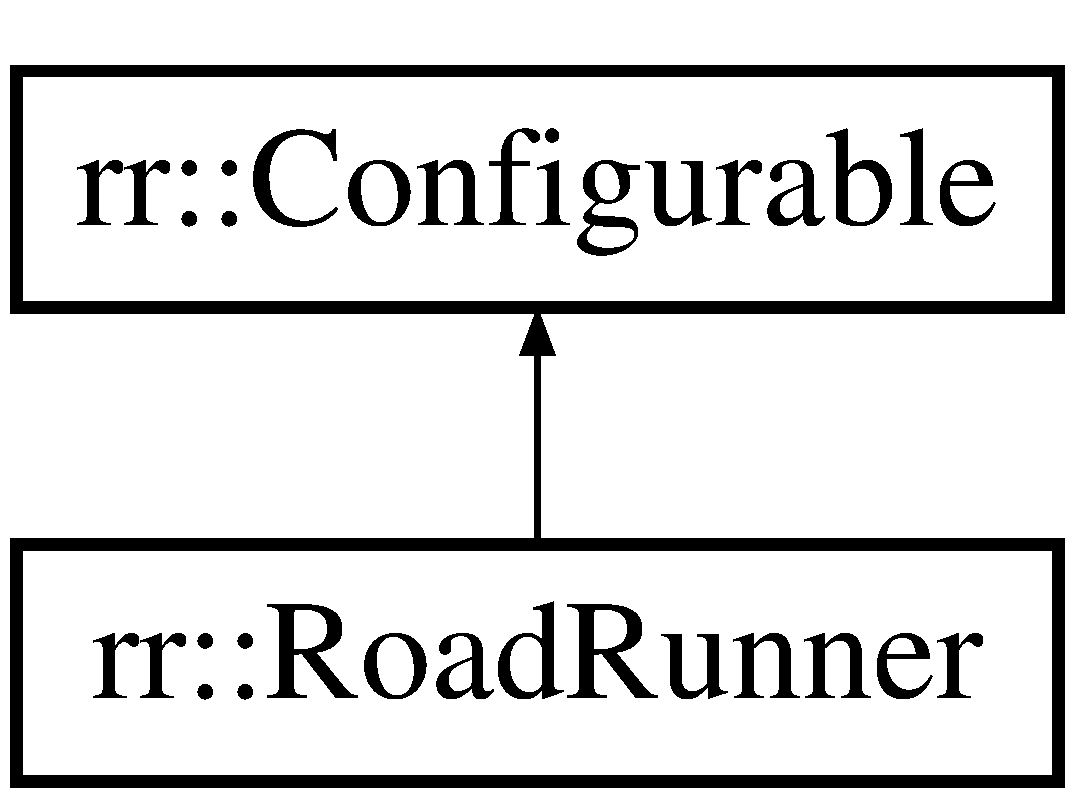
\includegraphics[height=2.000000cm]{classrr_1_1_configurable}
\end{center}
\end{figure}
\subsection*{Public Member Functions}
\begin{DoxyCompactItemize}
\item 
virtual \-\_\-xml\-Node $\ast$ \hyperlink{classrr_1_1_configurable_af1eeec76874dccc105e70f5fd2255df3}{create\-Config\-Node} ()=0
\item 
virtual void \hyperlink{classrr_1_1_configurable_add9f6002952f1d4a4672ead64b5821ab}{load\-Config} (const \-\_\-xml\-Doc $\ast$doc)=0
\end{DoxyCompactItemize}
\subsection*{Static Public Member Functions}
\begin{DoxyCompactItemize}
\item 
static void \hyperlink{classrr_1_1_configurable_aa3ecf478d5b6ef58967ff45dd13623d2}{load\-Xml\-Config} (const std\-::string \&xml, \hyperlink{classrr_1_1_configurable}{Configurable} $\ast$configurable)
\item 
static std\-::string \hyperlink{classrr_1_1_configurable_a326b7f6db697fb213908234b0135b93b}{xml\-From\-Config\-Node} (\-\_\-xml\-Node $\ast$config)
\item 
static \-\_\-xml\-Node $\ast$ \hyperlink{classrr_1_1_configurable_a1cf1d4c3086683eb8ba5e326f90eb9dd}{create\-Capability\-Node} (const std\-::string \&name, const std\-::string \&method, const std\-::string \&desc)
\item 
static \-\_\-xml\-Node $\ast$ \hyperlink{classrr_1_1_configurable_a8b2199153c22d156ead39f72955f5911}{create\-Capabilities\-Node} (const std\-::string \&name, const std\-::string \&desc)
\item 
static \-\_\-xml\-Node $\ast$ \hyperlink{classrr_1_1_configurable_ad25336b103d9821c24be9131b5be65db}{add\-Child} (\-\_\-xml\-Node $\ast$parent, \-\_\-xml\-Node $\ast$cur)
\item 
static \-\_\-xml\-Node $\ast$ \hyperlink{classrr_1_1_configurable_ab4b9e1d503929f9852c193a3109f4fd1}{create\-Parameter\-Node} (const std\-::string \&name, const std\-::string \&hint, const std\-::string \&value)
\item 
static \-\_\-xml\-Node $\ast$ \hyperlink{classrr_1_1_configurable_a98ac3ed5609f816743b4001eab12a15e}{create\-Parameter\-Node} (const std\-::string \&name, const std\-::string \&hint, int value)
\item 
static \-\_\-xml\-Node $\ast$ \hyperlink{classrr_1_1_configurable_a9549b987e35cebb539e06fe05c7bdedb}{create\-Parameter\-Node} (const std\-::string \&name, const std\-::string \&hint, double value)
\item 
static std\-::string \hyperlink{classrr_1_1_configurable_affc794880c1fa037539465ca703ebd1f}{get\-Parameter\-String\-Value} (const \-\_\-xml\-Doc $\ast$doc, const std\-::string \&capability\-Name, const std\-::string \&parameter\-Name)
\item 
static int \hyperlink{classrr_1_1_configurable_ac64a27f007da8352b045495224724592}{get\-Parameter\-Int\-Value} (const \-\_\-xml\-Doc $\ast$doc, const std\-::string \&capability\-Name, const std\-::string \&parameter\-Name)
\item 
static double \hyperlink{classrr_1_1_configurable_afbbe4dea6032d20b303f58fe5cb6dc6f}{get\-Parameter\-Double\-Value} (const \-\_\-xml\-Doc $\ast$doc, const std\-::string \&capability\-Name, const std\-::string \&parameter\-Name)
\end{DoxyCompactItemize}


\subsection{Detailed Description}
The \hyperlink{classrr_1_1_road_runner}{Road\-Runner} configuration system allows a collection of potentially disparate objects to have all of thier configuration parameters collected and assembled into a single xml document.

The hierarchy of \hyperlink{classrr_1_1_configurable}{Configurable} maintians no additional state other than the local configuration parameters of each terminal node and the parent -\/ child relationships. The xml document / nodes exists only for the lifetime of the create\-Config\-Node / load\-Config calls. No xml objects should ever be maintined outside these method calls.

There are two method in the \hyperlink{classrr_1_1_configurable}{Configurable} interface, one returns a configuration as an xml node the other allows the object to load or read its configuration from an xml document.

Classes that implment this interface must return either a capabilities, capability or parameter node. The static add\-Child function will automatically determine what type the child and parents are and add it in the appropriate location. So for example, say the both the parent and child nodes are 'cababities', in this case, the list of 'cabability' elements is pulled from the child and appended to the parent's capabitiles node as child nodes. This situation is encountered when a Plugin\-Manager is used. \hyperlink{classrr_1_1_road_runner}{Road\-Runner} does not require nor is even aware of a Plugin\-Manager. \hyperlink{classrr_1_1_road_runner}{Road\-Runner} considers itself a top level object thus returns a 'capabilities' node. The Plugin\-Manager contains a \hyperlink{classrr_1_1_road_runner}{Road\-Runner} object, so when the Plugin\-Manager creates a 'cababilities' node, asks all of its plugins for a config, these are typically a 'cabability' which are added to the 'cababities' node that the Plugin\-Manager created. The Plugin\-Manager also asks \hyperlink{classrr_1_1_road_runner}{Road\-Runner} for its capabilities, so in this case, \hyperlink{classrr_1_1_road_runner}{Road\-Runner}'s set of cabability nodes are automatically appended to the Plugin\-Manager's cababity nodes and a single combined document is returned. 

\subsection{Member Function Documentation}
\hypertarget{classrr_1_1_configurable_ad25336b103d9821c24be9131b5be65db}{\index{rr\-::\-Configurable@{rr\-::\-Configurable}!add\-Child@{add\-Child}}
\index{add\-Child@{add\-Child}!rr::Configurable@{rr\-::\-Configurable}}
\subsubsection[{add\-Child}]{\setlength{\rightskip}{0pt plus 5cm}xml\-Node $\ast$ rr\-::\-Configurable\-::add\-Child (
\begin{DoxyParamCaption}
\item[{\-\_\-xml\-Node $\ast$}]{parent, }
\item[{\-\_\-xml\-Node $\ast$}]{cur}
\end{DoxyParamCaption}
)\hspace{0.3cm}{\ttfamily [static]}}}\label{classrr_1_1_configurable_ad25336b103d9821c24be9131b5be65db}
essentially just calls xml\-Add\-Child, but performs some checking to verify that a parameter can only be added to a capability and a capabilty can only be added to a capabilities node.

as usual, the parent takes ownership of the child node. \hypertarget{classrr_1_1_configurable_a8b2199153c22d156ead39f72955f5911}{\index{rr\-::\-Configurable@{rr\-::\-Configurable}!create\-Capabilities\-Node@{create\-Capabilities\-Node}}
\index{create\-Capabilities\-Node@{create\-Capabilities\-Node}!rr::Configurable@{rr\-::\-Configurable}}
\subsubsection[{create\-Capabilities\-Node}]{\setlength{\rightskip}{0pt plus 5cm}xml\-Node $\ast$ rr\-::\-Configurable\-::create\-Capabilities\-Node (
\begin{DoxyParamCaption}
\item[{const std\-::string \&}]{name, }
\item[{const std\-::string \&}]{desc}
\end{DoxyParamCaption}
)\hspace{0.3cm}{\ttfamily [static]}}}\label{classrr_1_1_configurable_a8b2199153c22d156ead39f72955f5911}
create a \char`\"{}capabilities\char`\"{} node with \char`\"{}name\char`\"{} and \char`\"{}description\char`\"{} attributes. \hypertarget{classrr_1_1_configurable_a1cf1d4c3086683eb8ba5e326f90eb9dd}{\index{rr\-::\-Configurable@{rr\-::\-Configurable}!create\-Capability\-Node@{create\-Capability\-Node}}
\index{create\-Capability\-Node@{create\-Capability\-Node}!rr::Configurable@{rr\-::\-Configurable}}
\subsubsection[{create\-Capability\-Node}]{\setlength{\rightskip}{0pt plus 5cm}xml\-Node $\ast$ rr\-::\-Configurable\-::create\-Capability\-Node (
\begin{DoxyParamCaption}
\item[{const std\-::string \&}]{name, }
\item[{const std\-::string \&}]{method, }
\item[{const std\-::string \&}]{desc}
\end{DoxyParamCaption}
)\hspace{0.3cm}{\ttfamily [static]}}}\label{classrr_1_1_configurable_a1cf1d4c3086683eb8ba5e326f90eb9dd}
create a \char`\"{}capability\char`\"{} node with \char`\"{}name\char`\"{}, \char`\"{}method\char`\"{} and \char`\"{}description\char`\"{} atttibutes. \hypertarget{classrr_1_1_configurable_af1eeec76874dccc105e70f5fd2255df3}{\index{rr\-::\-Configurable@{rr\-::\-Configurable}!create\-Config\-Node@{create\-Config\-Node}}
\index{create\-Config\-Node@{create\-Config\-Node}!rr::Configurable@{rr\-::\-Configurable}}
\subsubsection[{create\-Config\-Node}]{\setlength{\rightskip}{0pt plus 5cm}virtual \-\_\-xml\-Node$\ast$ rr\-::\-Configurable\-::create\-Config\-Node (
\begin{DoxyParamCaption}
{}
\end{DoxyParamCaption}
)\hspace{0.3cm}{\ttfamily [pure virtual]}}}\label{classrr_1_1_configurable_af1eeec76874dccc105e70f5fd2255df3}
creates a new xml element that represent the current state of this \hyperlink{classrr_1_1_configurable}{Configurable} object and all if its child objects. 

Implemented in \hyperlink{classrr_1_1_road_runner_afd5401ecd63ac9dda2fe52f98066cb23}{rr\-::\-Road\-Runner}.

\hypertarget{classrr_1_1_configurable_ab4b9e1d503929f9852c193a3109f4fd1}{\index{rr\-::\-Configurable@{rr\-::\-Configurable}!create\-Parameter\-Node@{create\-Parameter\-Node}}
\index{create\-Parameter\-Node@{create\-Parameter\-Node}!rr::Configurable@{rr\-::\-Configurable}}
\subsubsection[{create\-Parameter\-Node}]{\setlength{\rightskip}{0pt plus 5cm}xml\-Node $\ast$ rr\-::\-Configurable\-::create\-Parameter\-Node (
\begin{DoxyParamCaption}
\item[{const std\-::string \&}]{name, }
\item[{const std\-::string \&}]{hint, }
\item[{const std\-::string \&}]{value}
\end{DoxyParamCaption}
)\hspace{0.3cm}{\ttfamily [static]}}}\label{classrr_1_1_configurable_ab4b9e1d503929f9852c193a3109f4fd1}
create a \char`\"{}parameter\char`\"{} node with a 'string' value. \hypertarget{classrr_1_1_configurable_a98ac3ed5609f816743b4001eab12a15e}{\index{rr\-::\-Configurable@{rr\-::\-Configurable}!create\-Parameter\-Node@{create\-Parameter\-Node}}
\index{create\-Parameter\-Node@{create\-Parameter\-Node}!rr::Configurable@{rr\-::\-Configurable}}
\subsubsection[{create\-Parameter\-Node}]{\setlength{\rightskip}{0pt plus 5cm}xml\-Node $\ast$ rr\-::\-Configurable\-::create\-Parameter\-Node (
\begin{DoxyParamCaption}
\item[{const std\-::string \&}]{name, }
\item[{const std\-::string \&}]{hint, }
\item[{int}]{value}
\end{DoxyParamCaption}
)\hspace{0.3cm}{\ttfamily [static]}}}\label{classrr_1_1_configurable_a98ac3ed5609f816743b4001eab12a15e}
create a \char`\"{}parameter\char`\"{} node with a 'integer' value. \hypertarget{classrr_1_1_configurable_a9549b987e35cebb539e06fe05c7bdedb}{\index{rr\-::\-Configurable@{rr\-::\-Configurable}!create\-Parameter\-Node@{create\-Parameter\-Node}}
\index{create\-Parameter\-Node@{create\-Parameter\-Node}!rr::Configurable@{rr\-::\-Configurable}}
\subsubsection[{create\-Parameter\-Node}]{\setlength{\rightskip}{0pt plus 5cm}xml\-Node $\ast$ rr\-::\-Configurable\-::create\-Parameter\-Node (
\begin{DoxyParamCaption}
\item[{const std\-::string \&}]{name, }
\item[{const std\-::string \&}]{hint, }
\item[{double}]{value}
\end{DoxyParamCaption}
)\hspace{0.3cm}{\ttfamily [static]}}}\label{classrr_1_1_configurable_a9549b987e35cebb539e06fe05c7bdedb}
create a \char`\"{}parameter\char`\"{} node with a 'double' value. \hypertarget{classrr_1_1_configurable_afbbe4dea6032d20b303f58fe5cb6dc6f}{\index{rr\-::\-Configurable@{rr\-::\-Configurable}!get\-Parameter\-Double\-Value@{get\-Parameter\-Double\-Value}}
\index{get\-Parameter\-Double\-Value@{get\-Parameter\-Double\-Value}!rr::Configurable@{rr\-::\-Configurable}}
\subsubsection[{get\-Parameter\-Double\-Value}]{\setlength{\rightskip}{0pt plus 5cm}double rr\-::\-Configurable\-::get\-Parameter\-Double\-Value (
\begin{DoxyParamCaption}
\item[{const \-\_\-xml\-Doc $\ast$}]{doc, }
\item[{const std\-::string \&}]{capability\-Name, }
\item[{const std\-::string \&}]{parameter\-Name}
\end{DoxyParamCaption}
)\hspace{0.3cm}{\ttfamily [static]}}}\label{classrr_1_1_configurable_afbbe4dea6032d20b303f58fe5cb6dc6f}
find the parameter node for the given capability / parameter in the xml configuration document and coerce the value to a double.


\begin{DoxyExceptions}{Exceptions}
{\em std\-::exception} & on failure. \\
\hline
\end{DoxyExceptions}
\hypertarget{classrr_1_1_configurable_ac64a27f007da8352b045495224724592}{\index{rr\-::\-Configurable@{rr\-::\-Configurable}!get\-Parameter\-Int\-Value@{get\-Parameter\-Int\-Value}}
\index{get\-Parameter\-Int\-Value@{get\-Parameter\-Int\-Value}!rr::Configurable@{rr\-::\-Configurable}}
\subsubsection[{get\-Parameter\-Int\-Value}]{\setlength{\rightskip}{0pt plus 5cm}int rr\-::\-Configurable\-::get\-Parameter\-Int\-Value (
\begin{DoxyParamCaption}
\item[{const \-\_\-xml\-Doc $\ast$}]{doc, }
\item[{const std\-::string \&}]{capability\-Name, }
\item[{const std\-::string \&}]{parameter\-Name}
\end{DoxyParamCaption}
)\hspace{0.3cm}{\ttfamily [static]}}}\label{classrr_1_1_configurable_ac64a27f007da8352b045495224724592}
find the parameter node for the given capability / parameter in the xml configuration document and coerce the value to an integer.


\begin{DoxyExceptions}{Exceptions}
{\em std\-::exception} & on failure. \\
\hline
\end{DoxyExceptions}
\hypertarget{classrr_1_1_configurable_affc794880c1fa037539465ca703ebd1f}{\index{rr\-::\-Configurable@{rr\-::\-Configurable}!get\-Parameter\-String\-Value@{get\-Parameter\-String\-Value}}
\index{get\-Parameter\-String\-Value@{get\-Parameter\-String\-Value}!rr::Configurable@{rr\-::\-Configurable}}
\subsubsection[{get\-Parameter\-String\-Value}]{\setlength{\rightskip}{0pt plus 5cm}std\-::string rr\-::\-Configurable\-::get\-Parameter\-String\-Value (
\begin{DoxyParamCaption}
\item[{const \-\_\-xml\-Doc $\ast$}]{doc, }
\item[{const std\-::string \&}]{capability\-Name, }
\item[{const std\-::string \&}]{parameter\-Name}
\end{DoxyParamCaption}
)\hspace{0.3cm}{\ttfamily [static]}}}\label{classrr_1_1_configurable_affc794880c1fa037539465ca703ebd1f}
find the parameter node for the given capability / parameter in the xml configuration document and return its value.


\begin{DoxyExceptions}{Exceptions}
{\em std\-::exception} & on failure. \\
\hline
\end{DoxyExceptions}
\hypertarget{classrr_1_1_configurable_add9f6002952f1d4a4672ead64b5821ab}{\index{rr\-::\-Configurable@{rr\-::\-Configurable}!load\-Config@{load\-Config}}
\index{load\-Config@{load\-Config}!rr::Configurable@{rr\-::\-Configurable}}
\subsubsection[{load\-Config}]{\setlength{\rightskip}{0pt plus 5cm}virtual void rr\-::\-Configurable\-::load\-Config (
\begin{DoxyParamCaption}
\item[{const \-\_\-xml\-Doc $\ast$}]{doc}
\end{DoxyParamCaption}
)\hspace{0.3cm}{\ttfamily [pure virtual]}}}\label{classrr_1_1_configurable_add9f6002952f1d4a4672ead64b5821ab}
Given an xml element, the \hyperlink{classrr_1_1_configurable}{Configurable} object should pick its needed values that are stored in the element and use them to set its internal configuration state. 

Implemented in \hyperlink{classrr_1_1_road_runner_aac7ee8e64b2709d5d5a7e9b0cff8acc7}{rr\-::\-Road\-Runner}.

\hypertarget{classrr_1_1_configurable_aa3ecf478d5b6ef58967ff45dd13623d2}{\index{rr\-::\-Configurable@{rr\-::\-Configurable}!load\-Xml\-Config@{load\-Xml\-Config}}
\index{load\-Xml\-Config@{load\-Xml\-Config}!rr::Configurable@{rr\-::\-Configurable}}
\subsubsection[{load\-Xml\-Config}]{\setlength{\rightskip}{0pt plus 5cm}void rr\-::\-Configurable\-::load\-Xml\-Config (
\begin{DoxyParamCaption}
\item[{const std\-::string \&}]{xml, }
\item[{{\bf Configurable} $\ast$}]{configurable}
\end{DoxyParamCaption}
)\hspace{0.3cm}{\ttfamily [static]}}}\label{classrr_1_1_configurable_aa3ecf478d5b6ef58967ff45dd13623d2}
given an xml string, this loads the string into a document and calls load\-Config on the given configurable pointer with the root element.

Also checks that the root element is a \char`\"{}capabilties\char`\"{} element. \hypertarget{classrr_1_1_configurable_a326b7f6db697fb213908234b0135b93b}{\index{rr\-::\-Configurable@{rr\-::\-Configurable}!xml\-From\-Config\-Node@{xml\-From\-Config\-Node}}
\index{xml\-From\-Config\-Node@{xml\-From\-Config\-Node}!rr::Configurable@{rr\-::\-Configurable}}
\subsubsection[{xml\-From\-Config\-Node}]{\setlength{\rightskip}{0pt plus 5cm}std\-::string rr\-::\-Configurable\-::xml\-From\-Config\-Node (
\begin{DoxyParamCaption}
\item[{\-\_\-xml\-Node $\ast$}]{config}
\end{DoxyParamCaption}
)\hspace{0.3cm}{\ttfamily [static]}}}\label{classrr_1_1_configurable_a326b7f6db697fb213908234b0135b93b}
Consumes an xml\-Node and creates a new document and sets this as the root node, The document takes ownership of the xml\-Node.

The document is then written out to a string which is returned, and the document is then finally freed. 

The documentation for this class was generated from the following files\-:\begin{DoxyCompactItemize}
\item 
source/Configurable.\-h\item 
source/Configurable.\-cpp\end{DoxyCompactItemize}

\hypertarget{classrr_1_1_core_exception}{\section{rr\-:\-:Core\-Exception Class Reference}
\label{classrr_1_1_core_exception}\index{rr\-::\-Core\-Exception@{rr\-::\-Core\-Exception}}
}
Inheritance diagram for rr\-:\-:Core\-Exception\-:\begin{figure}[H]
\begin{center}
\leavevmode
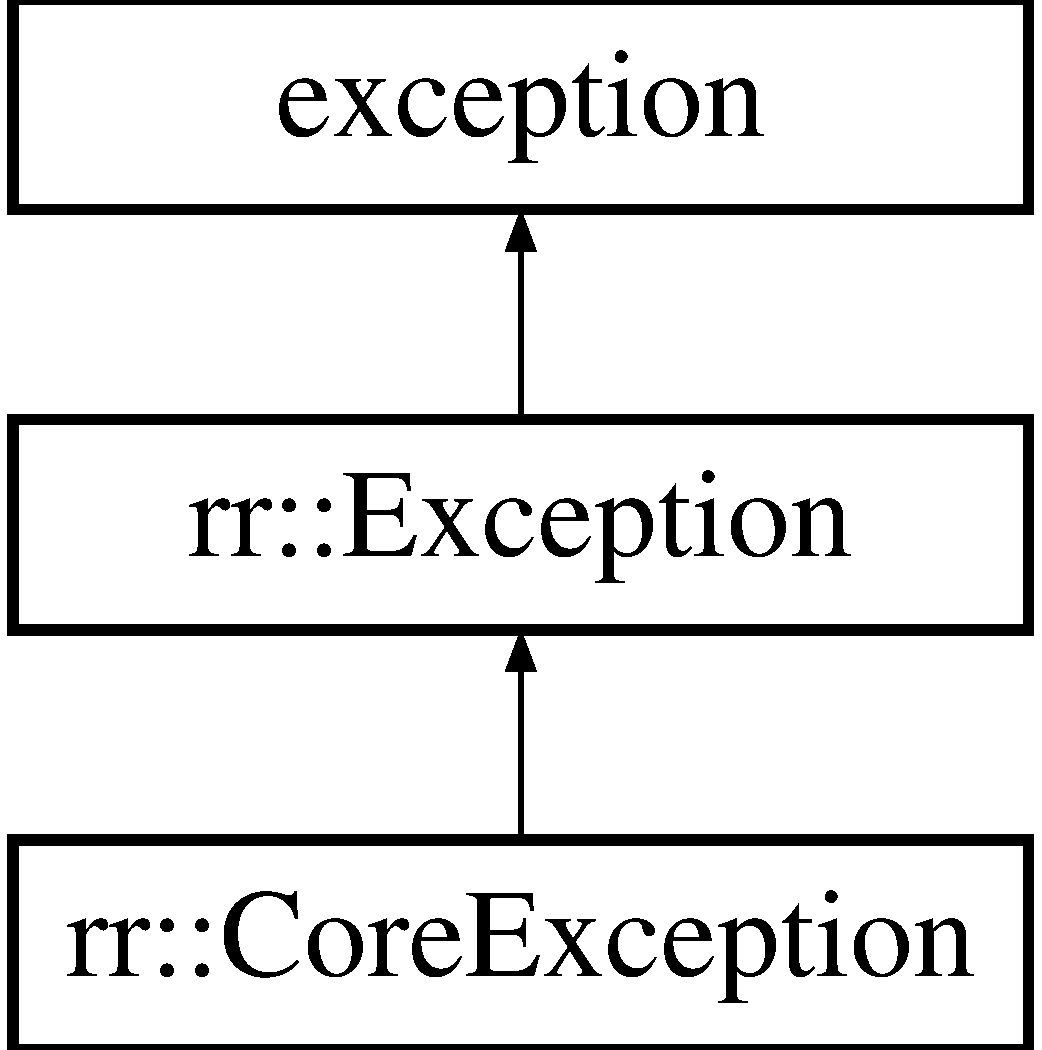
\includegraphics[height=3.000000cm]{classrr_1_1_core_exception}
\end{center}
\end{figure}
\subsection*{Public Member Functions}
\begin{DoxyCompactItemize}
\item 
\hypertarget{classrr_1_1_core_exception_aa5fae377d761664916e618a671512435}{{\bfseries Core\-Exception} (const string \&msg)}\label{classrr_1_1_core_exception_aa5fae377d761664916e618a671512435}

\item 
\hypertarget{classrr_1_1_core_exception_ae3db9042e1f7db934a2710a87649f4ff}{{\bfseries Core\-Exception} (const string \&msg1, const string \&msg2)}\label{classrr_1_1_core_exception_ae3db9042e1f7db934a2710a87649f4ff}

\end{DoxyCompactItemize}
\subsection*{Additional Inherited Members}


The documentation for this class was generated from the following files\-:\begin{DoxyCompactItemize}
\item 
source/rr\-Exception.\-h\item 
source/rr\-Exception.\-cpp\end{DoxyCompactItemize}

\hypertarget{classrr_1_1_c_v_o_d_e_exception}{\section{rr\-:\-:C\-V\-O\-D\-E\-Exception Class Reference}
\label{classrr_1_1_c_v_o_d_e_exception}\index{rr\-::\-C\-V\-O\-D\-E\-Exception@{rr\-::\-C\-V\-O\-D\-E\-Exception}}
}
Inheritance diagram for rr\-:\-:C\-V\-O\-D\-E\-Exception\-:\begin{figure}[H]
\begin{center}
\leavevmode
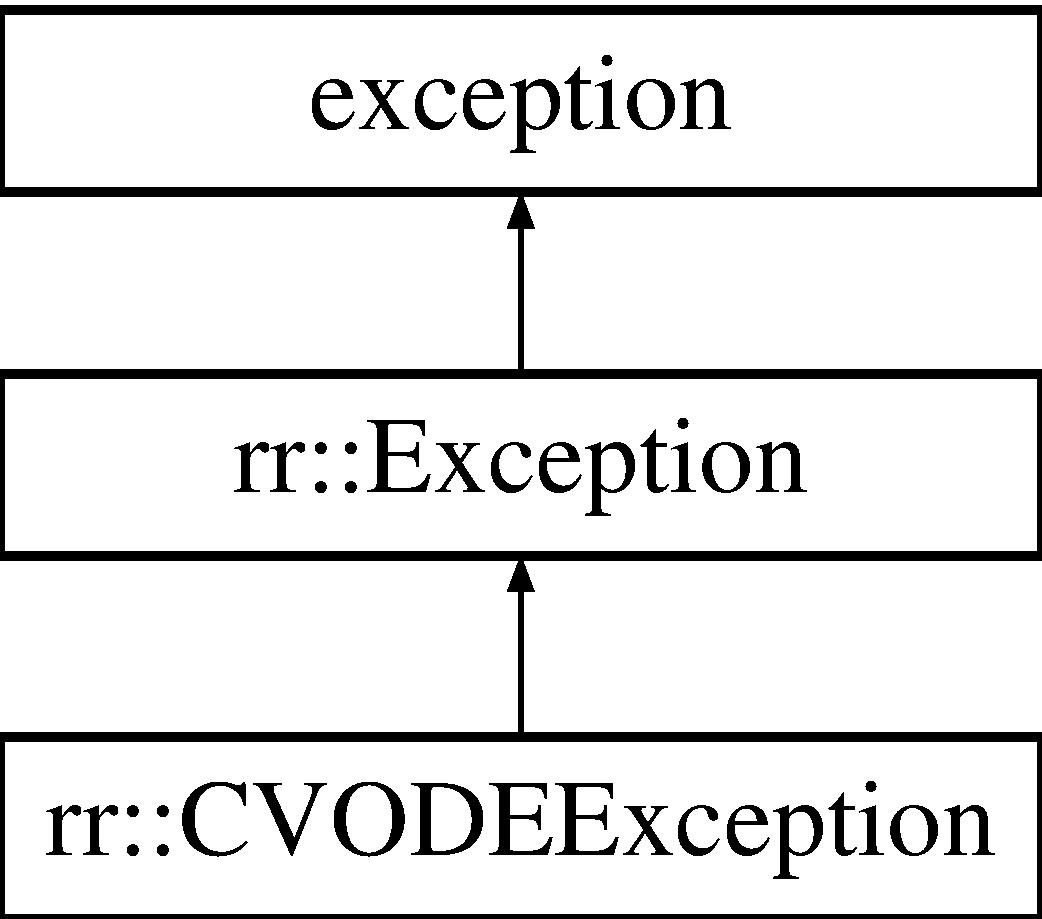
\includegraphics[height=3.000000cm]{classrr_1_1_c_v_o_d_e_exception}
\end{center}
\end{figure}
\subsection*{Public Member Functions}
\begin{DoxyCompactItemize}
\item 
\hypertarget{classrr_1_1_c_v_o_d_e_exception_a04b1bf996425851c6aa1b1ba70cb5ecb}{{\bfseries C\-V\-O\-D\-E\-Exception} (const string \&msg)}\label{classrr_1_1_c_v_o_d_e_exception_a04b1bf996425851c6aa1b1ba70cb5ecb}

\end{DoxyCompactItemize}
\subsection*{Additional Inherited Members}


The documentation for this class was generated from the following files\-:\begin{DoxyCompactItemize}
\item 
source/rr\-Exception.\-h\item 
source/rr\-Exception.\-cpp\end{DoxyCompactItemize}

\hypertarget{classrr_1_1_exception}{\section{rr\-:\-:Exception Class Reference}
\label{classrr_1_1_exception}\index{rr\-::\-Exception@{rr\-::\-Exception}}
}
Inheritance diagram for rr\-:\-:Exception\-:\begin{figure}[H]
\begin{center}
\leavevmode
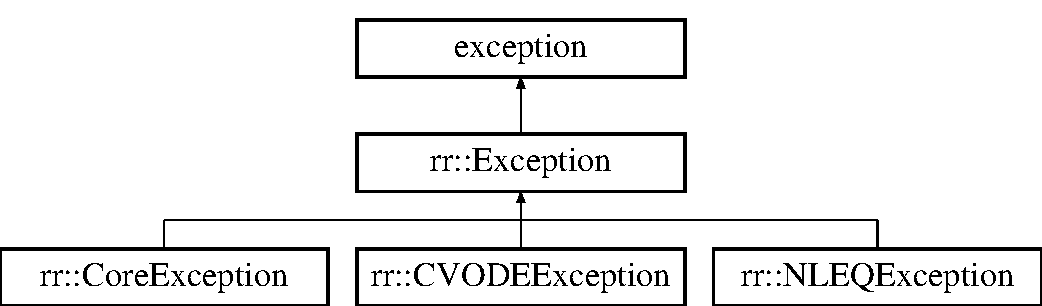
\includegraphics[height=3.000000cm]{classrr_1_1_exception}
\end{center}
\end{figure}
\subsection*{Public Member Functions}
\begin{DoxyCompactItemize}
\item 
\hypertarget{classrr_1_1_exception_a1eedd425af5fe42da04a373eaba4f63c}{{\bfseries Exception} (const string \&desc)}\label{classrr_1_1_exception_a1eedd425af5fe42da04a373eaba4f63c}

\item 
\hypertarget{classrr_1_1_exception_a1f34ebb35ae9b0cc8066b7b973b1c3a2}{virtual const char $\ast$ {\bfseries what} () const   throw ()}\label{classrr_1_1_exception_a1f34ebb35ae9b0cc8066b7b973b1c3a2}

\item 
\hypertarget{classrr_1_1_exception_affe28c5acce6e0e481d747f7798eb97a}{string {\bfseries Message} () const }\label{classrr_1_1_exception_affe28c5acce6e0e481d747f7798eb97a}

\item 
\hypertarget{classrr_1_1_exception_a297d246c83d1b5fc2fea62379e2dc139}{string {\bfseries get\-Message} () const }\label{classrr_1_1_exception_a297d246c83d1b5fc2fea62379e2dc139}

\end{DoxyCompactItemize}
\subsection*{Protected Attributes}
\begin{DoxyCompactItemize}
\item 
\hypertarget{classrr_1_1_exception_a6201902a23b56dab5704a726049a7908}{string {\bfseries m\-Message}}\label{classrr_1_1_exception_a6201902a23b56dab5704a726049a7908}

\end{DoxyCompactItemize}


The documentation for this class was generated from the following files\-:\begin{DoxyCompactItemize}
\item 
source/rr\-Exception.\-h\item 
source/rr\-Exception.\-cpp\end{DoxyCompactItemize}

\hypertarget{classrr_1_1_executable_model}{\section{rr\-:\-:Executable\-Model Class Reference}
\label{classrr_1_1_executable_model}\index{rr\-::\-Executable\-Model@{rr\-::\-Executable\-Model}}
}


{\ttfamily \#include $<$rr\-Executable\-Model.\-h$>$}

\subsection*{Public Member Functions}
\begin{DoxyCompactItemize}
\item 
virtual std\-::string \hyperlink{classrr_1_1_executable_model_a6ad7fd317a2335c337d7c8a3aeb8e044}{get\-Model\-Name} ()=0
\item 
\hypertarget{classrr_1_1_executable_model_ad38c7e2bf987ce1f7cbb8ac7316b8760}{virtual void {\bfseries set\-Time} (double \-\_\-time)=0}\label{classrr_1_1_executable_model_ad38c7e2bf987ce1f7cbb8ac7316b8760}

\item 
\hypertarget{classrr_1_1_executable_model_a9f4ae8c898f3c1553377b0f90b96c8e4}{virtual double {\bfseries get\-Time} ()=0}\label{classrr_1_1_executable_model_a9f4ae8c898f3c1553377b0f90b96c8e4}

\item 
\hypertarget{classrr_1_1_executable_model_a78d7c7496f2452280933a50057d2cda4}{virtual bool {\bfseries get\-Conserved\-Sum\-Changed} ()=0}\label{classrr_1_1_executable_model_a78d7c7496f2452280933a50057d2cda4}

\item 
\hypertarget{classrr_1_1_executable_model_a2294de2848a8411d7dacd62caeb8963e}{virtual void {\bfseries set\-Conserved\-Sum\-Changed} (bool)=0}\label{classrr_1_1_executable_model_a2294de2848a8411d7dacd62caeb8963e}

\item 
virtual void \hyperlink{classrr_1_1_executable_model_ae87772afeacb710067c2dd7a53106694}{eval\-Initial\-Conditions} ()=0
\item 
virtual void \hyperlink{classrr_1_1_executable_model_a217c61819d9b029c5928ace53b805e89}{reset} ()=0
\item 
\hypertarget{classrr_1_1_executable_model_af347779e832d6eaa7c263023b8d16739}{virtual int {\bfseries get\-Num\-Independent\-Species} ()=0}\label{classrr_1_1_executable_model_af347779e832d6eaa7c263023b8d16739}

\item 
\hypertarget{classrr_1_1_executable_model_a5654c9ac88bf580d0f8be22c4feb4e3b}{virtual int {\bfseries get\-Num\-Dependent\-Species} ()=0}\label{classrr_1_1_executable_model_a5654c9ac88bf580d0f8be22c4feb4e3b}

\item 
\hypertarget{classrr_1_1_executable_model_aa2999a84a5a0d691dc08f3f78b94636d}{virtual int {\bfseries get\-Num\-Floating\-Species} ()=0}\label{classrr_1_1_executable_model_aa2999a84a5a0d691dc08f3f78b94636d}

\item 
\hypertarget{classrr_1_1_executable_model_a390a1905aabac6056f6dceff11833c43}{virtual int {\bfseries get\-Floating\-Species\-Index} (const std\-::string \&eid)=0}\label{classrr_1_1_executable_model_a390a1905aabac6056f6dceff11833c43}

\item 
\hypertarget{classrr_1_1_executable_model_aed1e27797613d3d1814e793562c1651d}{virtual std\-::string {\bfseries get\-Floating\-Species\-Id} (int index)=0}\label{classrr_1_1_executable_model_aed1e27797613d3d1814e793562c1651d}

\item 
virtual int \hyperlink{classrr_1_1_executable_model_a6ee272090a6b7a4a6808f091c1930495}{get\-Num\-Boundary\-Species} ()=0
\item 
\hypertarget{classrr_1_1_executable_model_a28488139fa975776eded9e8c899c307d}{virtual int {\bfseries get\-Boundary\-Species\-Index} (const std\-::string \&eid)=0}\label{classrr_1_1_executable_model_a28488139fa975776eded9e8c899c307d}

\item 
\hypertarget{classrr_1_1_executable_model_ac63e324e4b7a5d73e46e5e8e6dde35ec}{virtual std\-::string {\bfseries get\-Boundary\-Species\-Id} (int index)=0}\label{classrr_1_1_executable_model_ac63e324e4b7a5d73e46e5e8e6dde35ec}

\item 
virtual int \hyperlink{classrr_1_1_executable_model_a02631a01d09aec3d02aca92cbebff2f0}{get\-Floating\-Species\-Amounts} (int len, int const $\ast$indx, double $\ast$values)=0
\item 
\hypertarget{classrr_1_1_executable_model_a25756080098404468d13fcff06c2b263}{virtual int {\bfseries set\-Floating\-Species\-Amounts} (int len, int const $\ast$indx, const double $\ast$values)=0}\label{classrr_1_1_executable_model_a25756080098404468d13fcff06c2b263}

\item 
\hypertarget{classrr_1_1_executable_model_a326d0bdea2730e5d1541decec396462c}{virtual int {\bfseries get\-Floating\-Species\-Amount\-Rates} (int len, int const $\ast$indx, double $\ast$values)=0}\label{classrr_1_1_executable_model_a326d0bdea2730e5d1541decec396462c}

\item 
virtual int \hyperlink{classrr_1_1_executable_model_a18aeea833f9db72a6f6beefb0c25f391}{get\-Floating\-Species\-Concentrations} (int len, int const $\ast$indx, double $\ast$values)=0
\item 
virtual int \hyperlink{classrr_1_1_executable_model_a42853a01cc2fae3b4a064d820ebacfaf}{set\-Floating\-Species\-Concentrations} (int len, int const $\ast$indx, double const $\ast$values)=0
\item 
virtual int \hyperlink{classrr_1_1_executable_model_a3a0b495144524d230defee08e58a5150}{set\-Floating\-Species\-Init\-Concentrations} (int len, int const $\ast$indx, double const $\ast$values)=0
\item 
virtual int \hyperlink{classrr_1_1_executable_model_a6521c4bfdb79c0b405a74fc4ccb67309}{get\-Floating\-Species\-Init\-Concentrations} (int len, int const $\ast$indx, double $\ast$values)=0
\item 
virtual int \hyperlink{classrr_1_1_executable_model_a0031c4cc30bf9329fb93f6d99d929669}{get\-Boundary\-Species\-Amounts} (int len, int const $\ast$indx, double $\ast$values)=0
\item 
virtual int \hyperlink{classrr_1_1_executable_model_a20e84c758da51167874aee3c66d8f576}{get\-Boundary\-Species\-Concentrations} (int len, int const $\ast$indx, double $\ast$values)=0
\item 
virtual int \hyperlink{classrr_1_1_executable_model_a4bb73d6d7076400f165335282b77524e}{set\-Boundary\-Species\-Concentrations} (int len, int const $\ast$indx, double const $\ast$values)=0
\item 
\hypertarget{classrr_1_1_executable_model_aabbf6f025ea3c064f0dcaa5e4afaa87e}{virtual int {\bfseries get\-Num\-Global\-Parameters} ()=0}\label{classrr_1_1_executable_model_aabbf6f025ea3c064f0dcaa5e4afaa87e}

\item 
\hypertarget{classrr_1_1_executable_model_abcdcc03c4563dfbe6b64f932812906ee}{virtual int {\bfseries get\-Global\-Parameter\-Index} (const std\-::string \&eid)=0}\label{classrr_1_1_executable_model_abcdcc03c4563dfbe6b64f932812906ee}

\item 
\hypertarget{classrr_1_1_executable_model_a2ad8bcf0faa7848e59e6b7234950dd59}{virtual std\-::string {\bfseries get\-Global\-Parameter\-Id} (int index)=0}\label{classrr_1_1_executable_model_a2ad8bcf0faa7848e59e6b7234950dd59}

\item 
virtual int \hyperlink{classrr_1_1_executable_model_aec13746ffbf2dcbc3467e05a9a73c2e4}{get\-Global\-Parameter\-Values} (int len, int const $\ast$indx, double $\ast$values)=0
\item 
\hypertarget{classrr_1_1_executable_model_a80f25d71380d0eb214601a3136382a35}{virtual int {\bfseries set\-Global\-Parameter\-Values} (int len, int const $\ast$indx, const double $\ast$values)=0}\label{classrr_1_1_executable_model_a80f25d71380d0eb214601a3136382a35}

\item 
\hypertarget{classrr_1_1_executable_model_acada1e982eafe06d0d5e46defdb40ca7}{virtual int {\bfseries get\-Num\-Compartments} ()=0}\label{classrr_1_1_executable_model_acada1e982eafe06d0d5e46defdb40ca7}

\item 
\hypertarget{classrr_1_1_executable_model_a366727be244766db2ff917b64949858c}{virtual int {\bfseries get\-Compartment\-Index} (const std\-::string \&eid)=0}\label{classrr_1_1_executable_model_a366727be244766db2ff917b64949858c}

\item 
\hypertarget{classrr_1_1_executable_model_a7b797c260c619f03761063f1863af2df}{virtual std\-::string {\bfseries get\-Compartment\-Id} (int index)=0}\label{classrr_1_1_executable_model_a7b797c260c619f03761063f1863af2df}

\item 
virtual int \hyperlink{classrr_1_1_executable_model_a1fe9ea6daf187a2a2dc83074c35d05ed}{get\-Compartment\-Volumes} (int len, int const $\ast$indx, double $\ast$values)=0
\item 
\hypertarget{classrr_1_1_executable_model_ae3b2f7000f709a92f78dbe78adfc992b}{virtual int {\bfseries set\-Compartment\-Volumes} (int len, int const $\ast$indx, const double $\ast$values)=0}\label{classrr_1_1_executable_model_ae3b2f7000f709a92f78dbe78adfc992b}

\item 
virtual double \hyperlink{classrr_1_1_executable_model_a24c46805c8c790f1cbec5c7726f03aa6}{get\-Stoichiometry} (int index)=0
\item 
\hypertarget{classrr_1_1_executable_model_ab1d58cc9a6bfd38851a3f42e08aa5a96}{virtual int {\bfseries get\-Num\-Conserved\-Sums} ()=0}\label{classrr_1_1_executable_model_ab1d58cc9a6bfd38851a3f42e08aa5a96}

\item 
\hypertarget{classrr_1_1_executable_model_af877de56a87fb2f2c1f13040d65d5518}{virtual int {\bfseries get\-Conserved\-Sum\-Index} (const std\-::string \&eid)=0}\label{classrr_1_1_executable_model_af877de56a87fb2f2c1f13040d65d5518}

\item 
\hypertarget{classrr_1_1_executable_model_a0bb2f514a22eb7e19928a74314435c98}{virtual std\-::string {\bfseries get\-Conserved\-Sum\-Id} (int index)=0}\label{classrr_1_1_executable_model_a0bb2f514a22eb7e19928a74314435c98}

\item 
\hypertarget{classrr_1_1_executable_model_ac083135eed08fa60a6351af41aaecde2}{virtual int {\bfseries get\-Conserved\-Sums} (int len, int const $\ast$indx, double $\ast$values)=0}\label{classrr_1_1_executable_model_ac083135eed08fa60a6351af41aaecde2}

\item 
\hypertarget{classrr_1_1_executable_model_adc8cb5d9f8cb8be0bc5ba4aaf082a55a}{virtual int {\bfseries set\-Conserved\-Sums} (int len, int const $\ast$indx, const double $\ast$values)=0}\label{classrr_1_1_executable_model_adc8cb5d9f8cb8be0bc5ba4aaf082a55a}

\item 
\hypertarget{classrr_1_1_executable_model_a8540961b62c8ad60ade60b77d1686f22}{virtual int {\bfseries get\-Num\-Rules} ()=0}\label{classrr_1_1_executable_model_a8540961b62c8ad60ade60b77d1686f22}

\item 
virtual int \hyperlink{classrr_1_1_executable_model_acb056a72125190c2abe39dba9c3600f1}{get\-Num\-Reactions} ()=0
\item 
virtual int \hyperlink{classrr_1_1_executable_model_a86fe96598b06cee5ca9a28dfdfd9d437}{get\-Reaction\-Index} (const std\-::string \&eid)=0
\item 
virtual std\-::string \hyperlink{classrr_1_1_executable_model_a230b955ef99e7616fb8d12c068b01f7b}{get\-Reaction\-Id} (int index)=0
\item 
\hypertarget{classrr_1_1_executable_model_ac814c5322dfcd876d0ffdcaa4eb88388}{virtual int {\bfseries get\-Reaction\-Rates} (int len, int const $\ast$indx, double $\ast$values)=0}\label{classrr_1_1_executable_model_ac814c5322dfcd876d0ffdcaa4eb88388}

\item 
virtual void \hyperlink{classrr_1_1_executable_model_a5e0e14f373b101b044559ec2c06a2a39}{eval\-Reaction\-Rates} ()=0
\item 
virtual void \hyperlink{classrr_1_1_executable_model_a119764cf63c094f8063ccac5f8190a80}{convert\-To\-Amounts} ()=0
\item 
\hypertarget{classrr_1_1_executable_model_a21fb68c451c822fa83c5b18a18ca4734}{virtual void {\bfseries compute\-Conserved\-Totals} ()=0}\label{classrr_1_1_executable_model_a21fb68c451c822fa83c5b18a18ca4734}

\item 
virtual void \hyperlink{classrr_1_1_executable_model_a2be036df6f2d85bb633e326c0e801f88}{set\-Rate\-Rule\-Values} (const double $\ast$rate\-Rule\-Values)=0
\item 
virtual void \hyperlink{classrr_1_1_executable_model_a8372872ec5858e91adc81080ad763c84}{get\-Rate\-Rule\-Values} (double $\ast$rate\-Rule\-Values)=0
\item 
virtual int \hyperlink{classrr_1_1_executable_model_a75b6f37ac538d2d2a0709fe4080b0570}{get\-State\-Vector} (double $\ast$state\-Vector)=0
\item 
virtual int \hyperlink{classrr_1_1_executable_model_a57a67063c957714b916d4a3d4277c3b9}{set\-State\-Vector} (const double $\ast$state\-Vector)=0
\item 
\hypertarget{classrr_1_1_executable_model_ad1e784a2f2f951fc1c74cde2ca26b893}{virtual void {\bfseries convert\-To\-Concentrations} ()=0}\label{classrr_1_1_executable_model_ad1e784a2f2f951fc1c74cde2ca26b893}

\item 
\hypertarget{classrr_1_1_executable_model_a3c46304cf254796fbf3ed73a5c7f0682}{virtual void {\bfseries update\-Dependent\-Species\-Values} ()=0}\label{classrr_1_1_executable_model_a3c46304cf254796fbf3ed73a5c7f0682}

\item 
\hypertarget{classrr_1_1_executable_model_a4e53afd18d5ce83c41176ffec519092c}{virtual void {\bfseries compute\-All\-Rates\-Of\-Change} ()=0}\label{classrr_1_1_executable_model_a4e53afd18d5ce83c41176ffec519092c}

\item 
virtual void \hyperlink{classrr_1_1_executable_model_a4f35c7ea16ac6e447eacd7d4a9e1a1a4}{eval\-Model} (double time, const double $\ast$y, double $\ast$dydt=0)=0
\item 
\hypertarget{classrr_1_1_executable_model_abe4be4ec2e96aaf0a256776dff3cc9a9}{virtual void {\bfseries test\-Constraints} ()=0}\label{classrr_1_1_executable_model_abe4be4ec2e96aaf0a256776dff3cc9a9}

\item 
\hypertarget{classrr_1_1_executable_model_ab8073e0f3e57cb6f0d807bdf60d1d2a1}{virtual std\-::string {\bfseries get\-Info} ()=0}\label{classrr_1_1_executable_model_ab8073e0f3e57cb6f0d807bdf60d1d2a1}

\item 
\hypertarget{classrr_1_1_executable_model_acea87cea26a0f322a8df7b5ae73f065c}{virtual void {\bfseries print} (std\-::ostream \&stream)=0}\label{classrr_1_1_executable_model_acea87cea26a0f322a8df7b5ae73f065c}

\item 
\hypertarget{classrr_1_1_executable_model_abd94b60defc6ffa9ab17166ebaa440c5}{virtual int {\bfseries get\-Num\-Events} ()=0}\label{classrr_1_1_executable_model_abd94b60defc6ffa9ab17166ebaa440c5}

\item 
virtual int \hyperlink{classrr_1_1_executable_model_a4dfbc74b5662469e050b8df80644e31a}{get\-Event\-Triggers} (int len, const int $\ast$indx, unsigned char $\ast$values)=0
\item 
\hypertarget{classrr_1_1_executable_model_ae5c185b8ec1688ee0c318736027236c0}{virtual void {\bfseries eval\-Events} (double time\-End, const unsigned char $\ast$previous\-Event\-Status, const double $\ast$initial\-State, double $\ast$final\-State)=0}\label{classrr_1_1_executable_model_ae5c185b8ec1688ee0c318736027236c0}

\item 
\hypertarget{classrr_1_1_executable_model_aac0678d1ec9fcea3eedfb480ee5c9a3b}{virtual int {\bfseries apply\-Pending\-Events} (const double $\ast$state\-Vector, double time\-End, double tout)=0}\label{classrr_1_1_executable_model_aac0678d1ec9fcea3eedfb480ee5c9a3b}

\item 
virtual void \hyperlink{classrr_1_1_executable_model_a7b6f43b8a273ac54aa5c8776c75bf1e2}{eval\-Event\-Roots} (double time, const double $\ast$y, double $\ast$gdot)=0
\item 
\hypertarget{classrr_1_1_executable_model_ad80b6a7167b0a78364dc680475ab2e3c}{virtual double {\bfseries get\-Next\-Pending\-Event\-Time} (bool pop)=0}\label{classrr_1_1_executable_model_ad80b6a7167b0a78364dc680475ab2e3c}

\item 
\hypertarget{classrr_1_1_executable_model_a9875c1203e09d4d51c29fdb2318f9a4c}{virtual int {\bfseries get\-Pending\-Event\-Size} ()=0}\label{classrr_1_1_executable_model_a9875c1203e09d4d51c29fdb2318f9a4c}

\item 
\hypertarget{classrr_1_1_executable_model_a936756fa4facd2b182b4cfcbe0f07fab}{virtual void {\bfseries reset\-Events} ()=0}\label{classrr_1_1_executable_model_a936756fa4facd2b182b4cfcbe0f07fab}

\item 
virtual \hyperlink{classrr_1_1_executable_model_a7d670c92b720d7dcf3ab70fa9d1b14d0}{$\sim$\-Executable\-Model} ()
\end{DoxyCompactItemize}


\subsection{Detailed Description}
The \hyperlink{classrr_1_1_executable_model}{Executable\-Model} interface provides a way to access an sbml model that was compiled, J\-I\-T'd or interpreted as executable (runnable) module.

An \hyperlink{classrr_1_1_executable_model}{Executable\-Model} holds a Model\-Data structure, all the simulation values are stored in the Model\-Data struct, i.\-e. the dynamic state of the model is fully contained in the Model\-Data structure.

An \hyperlink{classrr_1_1_executable_model}{Executable\-Model} shoud also contain all of the initial condisions, rules, functions and whatever other semantic information that was specified in the sbml model. 

\subsection{Constructor \& Destructor Documentation}
\hypertarget{classrr_1_1_executable_model_a7d670c92b720d7dcf3ab70fa9d1b14d0}{\index{rr\-::\-Executable\-Model@{rr\-::\-Executable\-Model}!$\sim$\-Executable\-Model@{$\sim$\-Executable\-Model}}
\index{$\sim$\-Executable\-Model@{$\sim$\-Executable\-Model}!rr::ExecutableModel@{rr\-::\-Executable\-Model}}
\subsubsection[{$\sim$\-Executable\-Model}]{\setlength{\rightskip}{0pt plus 5cm}virtual rr\-::\-Executable\-Model\-::$\sim$\-Executable\-Model (
\begin{DoxyParamCaption}
{}
\end{DoxyParamCaption}
)\hspace{0.3cm}{\ttfamily [inline]}, {\ttfamily [virtual]}}}\label{classrr_1_1_executable_model_a7d670c92b720d7dcf3ab70fa9d1b14d0}
need a virtual destructor as object implementing this interface can be deleted directly, i.\-e. \hyperlink{classrr_1_1_executable_model}{Executable\-Model} $\ast$p = create\-Model(...); delete p; 

\subsection{Member Function Documentation}
\hypertarget{classrr_1_1_executable_model_a119764cf63c094f8063ccac5f8190a80}{\index{rr\-::\-Executable\-Model@{rr\-::\-Executable\-Model}!convert\-To\-Amounts@{convert\-To\-Amounts}}
\index{convert\-To\-Amounts@{convert\-To\-Amounts}!rr::ExecutableModel@{rr\-::\-Executable\-Model}}
\subsubsection[{convert\-To\-Amounts}]{\setlength{\rightskip}{0pt plus 5cm}virtual void rr\-::\-Executable\-Model\-::convert\-To\-Amounts (
\begin{DoxyParamCaption}
{}
\end{DoxyParamCaption}
)\hspace{0.3cm}{\ttfamily [pure virtual]}}}\label{classrr_1_1_executable_model_a119764cf63c094f8063ccac5f8190a80}
sets the ammounts (Model\-Data\-::ammounts) by multipying the concentations (Model\-Data\-::y) by the compartment volume that the species belongs to.

Only for floating species. \hypertarget{classrr_1_1_executable_model_a7b6f43b8a273ac54aa5c8776c75bf1e2}{\index{rr\-::\-Executable\-Model@{rr\-::\-Executable\-Model}!eval\-Event\-Roots@{eval\-Event\-Roots}}
\index{eval\-Event\-Roots@{eval\-Event\-Roots}!rr::ExecutableModel@{rr\-::\-Executable\-Model}}
\subsubsection[{eval\-Event\-Roots}]{\setlength{\rightskip}{0pt plus 5cm}virtual void rr\-::\-Executable\-Model\-::eval\-Event\-Roots (
\begin{DoxyParamCaption}
\item[{double}]{time, }
\item[{const double $\ast$}]{y, }
\item[{double $\ast$}]{gdot}
\end{DoxyParamCaption}
)\hspace{0.3cm}{\ttfamily [pure virtual]}}}\label{classrr_1_1_executable_model_a7b6f43b8a273ac54aa5c8776c75bf1e2}
evaluate the event 'roots' -- when events transition form triggered -\/ non-\/triggered or triggered to non-\/triggered state.

Simplest method is to return 1 for triggered, -\/1 for not-\/triggered, so long as there is a zero crossing.


\begin{DoxyParams}{Parameters}
{\em time\mbox{[}in\mbox{]}} & current time \\
\hline
{\em y\mbox{[}in\mbox{]}} & the state vector \\
\hline
{\em gdot\mbox{[}out\mbox{]}} & result event roots, this is of length num\-Events. \\
\hline
\end{DoxyParams}
\hypertarget{classrr_1_1_executable_model_ae87772afeacb710067c2dd7a53106694}{\index{rr\-::\-Executable\-Model@{rr\-::\-Executable\-Model}!eval\-Initial\-Conditions@{eval\-Initial\-Conditions}}
\index{eval\-Initial\-Conditions@{eval\-Initial\-Conditions}!rr::ExecutableModel@{rr\-::\-Executable\-Model}}
\subsubsection[{eval\-Initial\-Conditions}]{\setlength{\rightskip}{0pt plus 5cm}virtual void rr\-::\-Executable\-Model\-::eval\-Initial\-Conditions (
\begin{DoxyParamCaption}
{}
\end{DoxyParamCaption}
)\hspace{0.3cm}{\ttfamily [pure virtual]}}}\label{classrr_1_1_executable_model_ae87772afeacb710067c2dd7a53106694}
evaluate the initial conditions specified in the sbml, this entails evaluating all Initial\-Assigments, Assigment\-Rules, initial values, etc...

Sets the the concentrations and ammounts to the values specified by the initial conditions, Model\-Data\-::floating\-Species\-Init\-Concentrations, i.\-e. the Model\-Data\-::floating\-Species\-Amounts\mbox{[}\-:\mbox{]} are set to Model\-Data\-::floating\-Species\-Init\-Concentrations\mbox{[}\-:\mbox{]} $\ast$ compartment volume, and Model\-Data\-::y\mbox{[}\-:\mbox{]} is set to Model\-Data\-::floating\-Species\-Init\-Concentrations\mbox{[}\-:\mbox{]}.

This sets the concentrations and ammounts to either initial\-Amount or initial\-Concentration (which ever exists) or 0 if they are missing. A later call to eval\-Initial\-Assignments will apply any initial\-Assigments to update the concentations and ammounts.

The the model state is fully set. \hypertarget{classrr_1_1_executable_model_a4f35c7ea16ac6e447eacd7d4a9e1a1a4}{\index{rr\-::\-Executable\-Model@{rr\-::\-Executable\-Model}!eval\-Model@{eval\-Model}}
\index{eval\-Model@{eval\-Model}!rr::ExecutableModel@{rr\-::\-Executable\-Model}}
\subsubsection[{eval\-Model}]{\setlength{\rightskip}{0pt plus 5cm}virtual void rr\-::\-Executable\-Model\-::eval\-Model (
\begin{DoxyParamCaption}
\item[{double}]{time, }
\item[{const double $\ast$}]{y, }
\item[{double $\ast$}]{dydt = {\ttfamily 0}}
\end{DoxyParamCaption}
)\hspace{0.3cm}{\ttfamily [pure virtual]}}}\label{classrr_1_1_executable_model_a4f35c7ea16ac6e447eacd7d4a9e1a1a4}
the state vector y is the rate rule values and floating species concentrations concatenated. y is of length num\-Floating\-Species + num\-Rate\-Rules.

The state vector is packed such that the first n raterule elements are the values of the rate rules, and the last n floatingspecies are the floating species values.


\begin{DoxyParams}[1]{Parameters}
\mbox{\tt in}  & {\em time} & current simulator time \\
\hline
\mbox{\tt in}  & {\em y} & state vector, must be either null, or have a size of that speciefied by get\-State\-Vector. If y is null, then the model is evaluated using its current state. If y is not null, then the y is considered the state vector. \\
\hline
\mbox{\tt out}  & {\em dydt} & calculated rate of change of the state vector, if null, it is ignored. \\
\hline
\end{DoxyParams}
\hypertarget{classrr_1_1_executable_model_a5e0e14f373b101b044559ec2c06a2a39}{\index{rr\-::\-Executable\-Model@{rr\-::\-Executable\-Model}!eval\-Reaction\-Rates@{eval\-Reaction\-Rates}}
\index{eval\-Reaction\-Rates@{eval\-Reaction\-Rates}!rr::ExecutableModel@{rr\-::\-Executable\-Model}}
\subsubsection[{eval\-Reaction\-Rates}]{\setlength{\rightskip}{0pt plus 5cm}virtual void rr\-::\-Executable\-Model\-::eval\-Reaction\-Rates (
\begin{DoxyParamCaption}
{}
\end{DoxyParamCaption}
)\hspace{0.3cm}{\ttfamily [pure virtual]}}}\label{classrr_1_1_executable_model_a5e0e14f373b101b044559ec2c06a2a39}
Evaluate the reaction rates using the current model state.

The reaction rates are stored in Model\-Data\-::reaction\-Rates. \hypertarget{classrr_1_1_executable_model_a0031c4cc30bf9329fb93f6d99d929669}{\index{rr\-::\-Executable\-Model@{rr\-::\-Executable\-Model}!get\-Boundary\-Species\-Amounts@{get\-Boundary\-Species\-Amounts}}
\index{get\-Boundary\-Species\-Amounts@{get\-Boundary\-Species\-Amounts}!rr::ExecutableModel@{rr\-::\-Executable\-Model}}
\subsubsection[{get\-Boundary\-Species\-Amounts}]{\setlength{\rightskip}{0pt plus 5cm}virtual int rr\-::\-Executable\-Model\-::get\-Boundary\-Species\-Amounts (
\begin{DoxyParamCaption}
\item[{int}]{len, }
\item[{int const $\ast$}]{indx, }
\item[{double $\ast$}]{values}
\end{DoxyParamCaption}
)\hspace{0.3cm}{\ttfamily [pure virtual]}}}\label{classrr_1_1_executable_model_a0031c4cc30bf9329fb93f6d99d929669}
get the boundary species amounts


\begin{DoxyParams}[1]{Parameters}
\mbox{\tt in}  & {\em len} & the length of the indx and values arrays. \\
\hline
\mbox{\tt in}  & {\em indx} & an array of length len of boundary species to return. \\
\hline
\mbox{\tt out}  & {\em values} & an array of at least length len which will store the returned boundary species amounts. \\
\hline
\end{DoxyParams}
\hypertarget{classrr_1_1_executable_model_a20e84c758da51167874aee3c66d8f576}{\index{rr\-::\-Executable\-Model@{rr\-::\-Executable\-Model}!get\-Boundary\-Species\-Concentrations@{get\-Boundary\-Species\-Concentrations}}
\index{get\-Boundary\-Species\-Concentrations@{get\-Boundary\-Species\-Concentrations}!rr::ExecutableModel@{rr\-::\-Executable\-Model}}
\subsubsection[{get\-Boundary\-Species\-Concentrations}]{\setlength{\rightskip}{0pt plus 5cm}virtual int rr\-::\-Executable\-Model\-::get\-Boundary\-Species\-Concentrations (
\begin{DoxyParamCaption}
\item[{int}]{len, }
\item[{int const $\ast$}]{indx, }
\item[{double $\ast$}]{values}
\end{DoxyParamCaption}
)\hspace{0.3cm}{\ttfamily [pure virtual]}}}\label{classrr_1_1_executable_model_a20e84c758da51167874aee3c66d8f576}
get the boundary species concentrations


\begin{DoxyParams}[1]{Parameters}
\mbox{\tt in}  & {\em len} & the length of the indx and values arrays. \\
\hline
\mbox{\tt in}  & {\em indx} & an array of length len of boundary species to return. \\
\hline
\mbox{\tt out}  & {\em values} & an array of at least length len which will store the returned boundary species amounts. \\
\hline
\end{DoxyParams}
\hypertarget{classrr_1_1_executable_model_a1fe9ea6daf187a2a2dc83074c35d05ed}{\index{rr\-::\-Executable\-Model@{rr\-::\-Executable\-Model}!get\-Compartment\-Volumes@{get\-Compartment\-Volumes}}
\index{get\-Compartment\-Volumes@{get\-Compartment\-Volumes}!rr::ExecutableModel@{rr\-::\-Executable\-Model}}
\subsubsection[{get\-Compartment\-Volumes}]{\setlength{\rightskip}{0pt plus 5cm}virtual int rr\-::\-Executable\-Model\-::get\-Compartment\-Volumes (
\begin{DoxyParamCaption}
\item[{int}]{len, }
\item[{int const $\ast$}]{indx, }
\item[{double $\ast$}]{values}
\end{DoxyParamCaption}
)\hspace{0.3cm}{\ttfamily [pure virtual]}}}\label{classrr_1_1_executable_model_a1fe9ea6daf187a2a2dc83074c35d05ed}
get the compartment volumes


\begin{DoxyParams}[1]{Parameters}
\mbox{\tt in}  & {\em len} & the length of the indx and values arrays. \\
\hline
\mbox{\tt in}  & {\em indx} & an array of length len of boundary species to return. \\
\hline
\mbox{\tt out}  & {\em values} & an array of at least length len which will store the returned boundary species amounts. \\
\hline
\end{DoxyParams}
\hypertarget{classrr_1_1_executable_model_a4dfbc74b5662469e050b8df80644e31a}{\index{rr\-::\-Executable\-Model@{rr\-::\-Executable\-Model}!get\-Event\-Triggers@{get\-Event\-Triggers}}
\index{get\-Event\-Triggers@{get\-Event\-Triggers}!rr::ExecutableModel@{rr\-::\-Executable\-Model}}
\subsubsection[{get\-Event\-Triggers}]{\setlength{\rightskip}{0pt plus 5cm}virtual int rr\-::\-Executable\-Model\-::get\-Event\-Triggers (
\begin{DoxyParamCaption}
\item[{int}]{len, }
\item[{const int $\ast$}]{indx, }
\item[{unsigned char $\ast$}]{values}
\end{DoxyParamCaption}
)\hspace{0.3cm}{\ttfamily [pure virtual]}}}\label{classrr_1_1_executable_model_a4dfbc74b5662469e050b8df80644e31a}
get the event status, false if the even is not triggered, true if it is.

The reason this returns an unsigned char instead of a bool array is this array is typically stuffed into an std\-::vector, and std\-::vector$<$bool$>$ is seriously broken and can not be used as a C array.

So, on every modern system I'm aware of, bool is an unsigned char, so use that data type here. \hypertarget{classrr_1_1_executable_model_a02631a01d09aec3d02aca92cbebff2f0}{\index{rr\-::\-Executable\-Model@{rr\-::\-Executable\-Model}!get\-Floating\-Species\-Amounts@{get\-Floating\-Species\-Amounts}}
\index{get\-Floating\-Species\-Amounts@{get\-Floating\-Species\-Amounts}!rr::ExecutableModel@{rr\-::\-Executable\-Model}}
\subsubsection[{get\-Floating\-Species\-Amounts}]{\setlength{\rightskip}{0pt plus 5cm}virtual int rr\-::\-Executable\-Model\-::get\-Floating\-Species\-Amounts (
\begin{DoxyParamCaption}
\item[{int}]{len, }
\item[{int const $\ast$}]{indx, }
\item[{double $\ast$}]{values}
\end{DoxyParamCaption}
)\hspace{0.3cm}{\ttfamily [pure virtual]}}}\label{classrr_1_1_executable_model_a02631a01d09aec3d02aca92cbebff2f0}
get the floating species amounts


\begin{DoxyParams}[1]{Parameters}
\mbox{\tt in}  & {\em len} & the length of the indx and values arrays. \\
\hline
\mbox{\tt in}  & {\em indx} & an array of length len of boundary species to return. \\
\hline
\mbox{\tt out}  & {\em values} & an array of at least length len which will store the returned boundary species amounts. \\
\hline
\end{DoxyParams}
\hypertarget{classrr_1_1_executable_model_a18aeea833f9db72a6f6beefb0c25f391}{\index{rr\-::\-Executable\-Model@{rr\-::\-Executable\-Model}!get\-Floating\-Species\-Concentrations@{get\-Floating\-Species\-Concentrations}}
\index{get\-Floating\-Species\-Concentrations@{get\-Floating\-Species\-Concentrations}!rr::ExecutableModel@{rr\-::\-Executable\-Model}}
\subsubsection[{get\-Floating\-Species\-Concentrations}]{\setlength{\rightskip}{0pt plus 5cm}virtual int rr\-::\-Executable\-Model\-::get\-Floating\-Species\-Concentrations (
\begin{DoxyParamCaption}
\item[{int}]{len, }
\item[{int const $\ast$}]{indx, }
\item[{double $\ast$}]{values}
\end{DoxyParamCaption}
)\hspace{0.3cm}{\ttfamily [pure virtual]}}}\label{classrr_1_1_executable_model_a18aeea833f9db72a6f6beefb0c25f391}
get the floating species concentrations


\begin{DoxyParams}[1]{Parameters}
\mbox{\tt in}  & {\em len} & the length of the indx and values arrays. \\
\hline
\mbox{\tt in}  & {\em indx} & an array of length len of boundary species to return. \\
\hline
\mbox{\tt out}  & {\em values} & an array of at least length len which will store the returned boundary species amounts. \\
\hline
\end{DoxyParams}
\hypertarget{classrr_1_1_executable_model_a6521c4bfdb79c0b405a74fc4ccb67309}{\index{rr\-::\-Executable\-Model@{rr\-::\-Executable\-Model}!get\-Floating\-Species\-Init\-Concentrations@{get\-Floating\-Species\-Init\-Concentrations}}
\index{get\-Floating\-Species\-Init\-Concentrations@{get\-Floating\-Species\-Init\-Concentrations}!rr::ExecutableModel@{rr\-::\-Executable\-Model}}
\subsubsection[{get\-Floating\-Species\-Init\-Concentrations}]{\setlength{\rightskip}{0pt plus 5cm}virtual int rr\-::\-Executable\-Model\-::get\-Floating\-Species\-Init\-Concentrations (
\begin{DoxyParamCaption}
\item[{int}]{len, }
\item[{int const $\ast$}]{indx, }
\item[{double $\ast$}]{values}
\end{DoxyParamCaption}
)\hspace{0.3cm}{\ttfamily [pure virtual]}}}\label{classrr_1_1_executable_model_a6521c4bfdb79c0b405a74fc4ccb67309}
pointless \hypertarget{classrr_1_1_executable_model_aec13746ffbf2dcbc3467e05a9a73c2e4}{\index{rr\-::\-Executable\-Model@{rr\-::\-Executable\-Model}!get\-Global\-Parameter\-Values@{get\-Global\-Parameter\-Values}}
\index{get\-Global\-Parameter\-Values@{get\-Global\-Parameter\-Values}!rr::ExecutableModel@{rr\-::\-Executable\-Model}}
\subsubsection[{get\-Global\-Parameter\-Values}]{\setlength{\rightskip}{0pt plus 5cm}virtual int rr\-::\-Executable\-Model\-::get\-Global\-Parameter\-Values (
\begin{DoxyParamCaption}
\item[{int}]{len, }
\item[{int const $\ast$}]{indx, }
\item[{double $\ast$}]{values}
\end{DoxyParamCaption}
)\hspace{0.3cm}{\ttfamily [pure virtual]}}}\label{classrr_1_1_executable_model_aec13746ffbf2dcbc3467e05a9a73c2e4}
get the global parameter values


\begin{DoxyParams}[1]{Parameters}
\mbox{\tt in}  & {\em len} & the length of the indx and values arrays. \\
\hline
\mbox{\tt in}  & {\em indx} & an array of length len of boundary species to return. \\
\hline
\mbox{\tt out}  & {\em values} & an array of at least length len which will store the returned boundary species amounts. \\
\hline
\end{DoxyParams}
\hypertarget{classrr_1_1_executable_model_a6ad7fd317a2335c337d7c8a3aeb8e044}{\index{rr\-::\-Executable\-Model@{rr\-::\-Executable\-Model}!get\-Model\-Name@{get\-Model\-Name}}
\index{get\-Model\-Name@{get\-Model\-Name}!rr::ExecutableModel@{rr\-::\-Executable\-Model}}
\subsubsection[{get\-Model\-Name}]{\setlength{\rightskip}{0pt plus 5cm}virtual std\-::string rr\-::\-Executable\-Model\-::get\-Model\-Name (
\begin{DoxyParamCaption}
{}
\end{DoxyParamCaption}
)\hspace{0.3cm}{\ttfamily [pure virtual]}}}\label{classrr_1_1_executable_model_a6ad7fd317a2335c337d7c8a3aeb8e044}
get the name of the model \hypertarget{classrr_1_1_executable_model_a6ee272090a6b7a4a6808f091c1930495}{\index{rr\-::\-Executable\-Model@{rr\-::\-Executable\-Model}!get\-Num\-Boundary\-Species@{get\-Num\-Boundary\-Species}}
\index{get\-Num\-Boundary\-Species@{get\-Num\-Boundary\-Species}!rr::ExecutableModel@{rr\-::\-Executable\-Model}}
\subsubsection[{get\-Num\-Boundary\-Species}]{\setlength{\rightskip}{0pt plus 5cm}virtual int rr\-::\-Executable\-Model\-::get\-Num\-Boundary\-Species (
\begin{DoxyParamCaption}
{}
\end{DoxyParamCaption}
)\hspace{0.3cm}{\ttfamily [pure virtual]}}}\label{classrr_1_1_executable_model_a6ee272090a6b7a4a6808f091c1930495}
get the number of boundary species. \hypertarget{classrr_1_1_executable_model_acb056a72125190c2abe39dba9c3600f1}{\index{rr\-::\-Executable\-Model@{rr\-::\-Executable\-Model}!get\-Num\-Reactions@{get\-Num\-Reactions}}
\index{get\-Num\-Reactions@{get\-Num\-Reactions}!rr::ExecutableModel@{rr\-::\-Executable\-Model}}
\subsubsection[{get\-Num\-Reactions}]{\setlength{\rightskip}{0pt plus 5cm}virtual int rr\-::\-Executable\-Model\-::get\-Num\-Reactions (
\begin{DoxyParamCaption}
{}
\end{DoxyParamCaption}
)\hspace{0.3cm}{\ttfamily [pure virtual]}}}\label{classrr_1_1_executable_model_acb056a72125190c2abe39dba9c3600f1}
get the number of reactions the model has \hypertarget{classrr_1_1_executable_model_a8372872ec5858e91adc81080ad763c84}{\index{rr\-::\-Executable\-Model@{rr\-::\-Executable\-Model}!get\-Rate\-Rule\-Values@{get\-Rate\-Rule\-Values}}
\index{get\-Rate\-Rule\-Values@{get\-Rate\-Rule\-Values}!rr::ExecutableModel@{rr\-::\-Executable\-Model}}
\subsubsection[{get\-Rate\-Rule\-Values}]{\setlength{\rightskip}{0pt plus 5cm}virtual void rr\-::\-Executable\-Model\-::get\-Rate\-Rule\-Values (
\begin{DoxyParamCaption}
\item[{double $\ast$}]{rate\-Rule\-Values}
\end{DoxyParamCaption}
)\hspace{0.3cm}{\ttfamily [pure virtual]}}}\label{classrr_1_1_executable_model_a8372872ec5858e91adc81080ad763c84}
get the 'values' i.\-e. the what the rate rule integrates to, and store it in the given array.

The length of rate\-Rule\-Values obviously must be the number of rate rules we have. \hypertarget{classrr_1_1_executable_model_a230b955ef99e7616fb8d12c068b01f7b}{\index{rr\-::\-Executable\-Model@{rr\-::\-Executable\-Model}!get\-Reaction\-Id@{get\-Reaction\-Id}}
\index{get\-Reaction\-Id@{get\-Reaction\-Id}!rr::ExecutableModel@{rr\-::\-Executable\-Model}}
\subsubsection[{get\-Reaction\-Id}]{\setlength{\rightskip}{0pt plus 5cm}virtual std\-::string rr\-::\-Executable\-Model\-::get\-Reaction\-Id (
\begin{DoxyParamCaption}
\item[{int}]{index}
\end{DoxyParamCaption}
)\hspace{0.3cm}{\ttfamily [pure virtual]}}}\label{classrr_1_1_executable_model_a230b955ef99e7616fb8d12c068b01f7b}
get the name of the specified reaction \hypertarget{classrr_1_1_executable_model_a86fe96598b06cee5ca9a28dfdfd9d437}{\index{rr\-::\-Executable\-Model@{rr\-::\-Executable\-Model}!get\-Reaction\-Index@{get\-Reaction\-Index}}
\index{get\-Reaction\-Index@{get\-Reaction\-Index}!rr::ExecutableModel@{rr\-::\-Executable\-Model}}
\subsubsection[{get\-Reaction\-Index}]{\setlength{\rightskip}{0pt plus 5cm}virtual int rr\-::\-Executable\-Model\-::get\-Reaction\-Index (
\begin{DoxyParamCaption}
\item[{const std\-::string \&}]{eid}
\end{DoxyParamCaption}
)\hspace{0.3cm}{\ttfamily [pure virtual]}}}\label{classrr_1_1_executable_model_a86fe96598b06cee5ca9a28dfdfd9d437}
get the index of a named reaction \begin{DoxyReturn}{Returns}
$>$= 0 on success, $<$ 0 on failure. 
\end{DoxyReturn}
\hypertarget{classrr_1_1_executable_model_a75b6f37ac538d2d2a0709fe4080b0570}{\index{rr\-::\-Executable\-Model@{rr\-::\-Executable\-Model}!get\-State\-Vector@{get\-State\-Vector}}
\index{get\-State\-Vector@{get\-State\-Vector}!rr::ExecutableModel@{rr\-::\-Executable\-Model}}
\subsubsection[{get\-State\-Vector}]{\setlength{\rightskip}{0pt plus 5cm}virtual int rr\-::\-Executable\-Model\-::get\-State\-Vector (
\begin{DoxyParamCaption}
\item[{double $\ast$}]{state\-Vector}
\end{DoxyParamCaption}
)\hspace{0.3cm}{\ttfamily [pure virtual]}}}\label{classrr_1_1_executable_model_a75b6f37ac538d2d2a0709fe4080b0570}
copies the internal model state vector into the provided buffer.


\begin{DoxyParams}[1]{Parameters}
\mbox{\tt out}  & {\em state\-Vector} & a buffer to copy the state vector into, if N\-U\-L\-L, return the size required.\\
\hline
\end{DoxyParams}
\begin{DoxyReturn}{Returns}
the number of items coppied into the provided buffer, if state\-Vector is N\-U\-L\-L, returns the length of the state vector. 
\end{DoxyReturn}
\hypertarget{classrr_1_1_executable_model_a24c46805c8c790f1cbec5c7726f03aa6}{\index{rr\-::\-Executable\-Model@{rr\-::\-Executable\-Model}!get\-Stoichiometry@{get\-Stoichiometry}}
\index{get\-Stoichiometry@{get\-Stoichiometry}!rr::ExecutableModel@{rr\-::\-Executable\-Model}}
\subsubsection[{get\-Stoichiometry}]{\setlength{\rightskip}{0pt plus 5cm}virtual double rr\-::\-Executable\-Model\-::get\-Stoichiometry (
\begin{DoxyParamCaption}
\item[{int}]{index}
\end{DoxyParamCaption}
)\hspace{0.3cm}{\ttfamily [pure virtual]}}}\label{classrr_1_1_executable_model_a24c46805c8c790f1cbec5c7726f03aa6}
no clue how this is supposed to work, here for compatibility \hypertarget{classrr_1_1_executable_model_a217c61819d9b029c5928ace53b805e89}{\index{rr\-::\-Executable\-Model@{rr\-::\-Executable\-Model}!reset@{reset}}
\index{reset@{reset}!rr::ExecutableModel@{rr\-::\-Executable\-Model}}
\subsubsection[{reset}]{\setlength{\rightskip}{0pt plus 5cm}virtual void rr\-::\-Executable\-Model\-::reset (
\begin{DoxyParamCaption}
{}
\end{DoxyParamCaption}
)\hspace{0.3cm}{\ttfamily [pure virtual]}}}\label{classrr_1_1_executable_model_a217c61819d9b029c5928ace53b805e89}
reset the model to its original state \hypertarget{classrr_1_1_executable_model_a4bb73d6d7076400f165335282b77524e}{\index{rr\-::\-Executable\-Model@{rr\-::\-Executable\-Model}!set\-Boundary\-Species\-Concentrations@{set\-Boundary\-Species\-Concentrations}}
\index{set\-Boundary\-Species\-Concentrations@{set\-Boundary\-Species\-Concentrations}!rr::ExecutableModel@{rr\-::\-Executable\-Model}}
\subsubsection[{set\-Boundary\-Species\-Concentrations}]{\setlength{\rightskip}{0pt plus 5cm}virtual int rr\-::\-Executable\-Model\-::set\-Boundary\-Species\-Concentrations (
\begin{DoxyParamCaption}
\item[{int}]{len, }
\item[{int const $\ast$}]{indx, }
\item[{double const $\ast$}]{values}
\end{DoxyParamCaption}
)\hspace{0.3cm}{\ttfamily [pure virtual]}}}\label{classrr_1_1_executable_model_a4bb73d6d7076400f165335282b77524e}
set the boundary species concentrations


\begin{DoxyParams}[1]{Parameters}
\mbox{\tt in}  & {\em len} & the length of the indx and values arrays. \\
\hline
\mbox{\tt in}  & {\em indx} & an array of length len of boundary species to return. \\
\hline
\mbox{\tt in}  & {\em values} & an array of at least length len which will store the returned boundary species amounts. \\
\hline
\end{DoxyParams}
\hypertarget{classrr_1_1_executable_model_a42853a01cc2fae3b4a064d820ebacfaf}{\index{rr\-::\-Executable\-Model@{rr\-::\-Executable\-Model}!set\-Floating\-Species\-Concentrations@{set\-Floating\-Species\-Concentrations}}
\index{set\-Floating\-Species\-Concentrations@{set\-Floating\-Species\-Concentrations}!rr::ExecutableModel@{rr\-::\-Executable\-Model}}
\subsubsection[{set\-Floating\-Species\-Concentrations}]{\setlength{\rightskip}{0pt plus 5cm}virtual int rr\-::\-Executable\-Model\-::set\-Floating\-Species\-Concentrations (
\begin{DoxyParamCaption}
\item[{int}]{len, }
\item[{int const $\ast$}]{indx, }
\item[{double const $\ast$}]{values}
\end{DoxyParamCaption}
)\hspace{0.3cm}{\ttfamily [pure virtual]}}}\label{classrr_1_1_executable_model_a42853a01cc2fae3b4a064d820ebacfaf}
set the floating species concentrations


\begin{DoxyParams}[1]{Parameters}
\mbox{\tt in}  & {\em len} & the length of the indx and values arrays. \\
\hline
\mbox{\tt in}  & {\em indx} & an array of length len of boundary species to return. \\
\hline
\mbox{\tt in}  & {\em values} & an array of at least length len which will store the returned boundary species amounts. \\
\hline
\end{DoxyParams}
\hypertarget{classrr_1_1_executable_model_a3a0b495144524d230defee08e58a5150}{\index{rr\-::\-Executable\-Model@{rr\-::\-Executable\-Model}!set\-Floating\-Species\-Init\-Concentrations@{set\-Floating\-Species\-Init\-Concentrations}}
\index{set\-Floating\-Species\-Init\-Concentrations@{set\-Floating\-Species\-Init\-Concentrations}!rr::ExecutableModel@{rr\-::\-Executable\-Model}}
\subsubsection[{set\-Floating\-Species\-Init\-Concentrations}]{\setlength{\rightskip}{0pt plus 5cm}virtual int rr\-::\-Executable\-Model\-::set\-Floating\-Species\-Init\-Concentrations (
\begin{DoxyParamCaption}
\item[{int}]{len, }
\item[{int const $\ast$}]{indx, }
\item[{double const $\ast$}]{values}
\end{DoxyParamCaption}
)\hspace{0.3cm}{\ttfamily [pure virtual]}}}\label{classrr_1_1_executable_model_a3a0b495144524d230defee08e58a5150}
a pointless method that will go away \hypertarget{classrr_1_1_executable_model_a2be036df6f2d85bb633e326c0e801f88}{\index{rr\-::\-Executable\-Model@{rr\-::\-Executable\-Model}!set\-Rate\-Rule\-Values@{set\-Rate\-Rule\-Values}}
\index{set\-Rate\-Rule\-Values@{set\-Rate\-Rule\-Values}!rr::ExecutableModel@{rr\-::\-Executable\-Model}}
\subsubsection[{set\-Rate\-Rule\-Values}]{\setlength{\rightskip}{0pt plus 5cm}virtual void rr\-::\-Executable\-Model\-::set\-Rate\-Rule\-Values (
\begin{DoxyParamCaption}
\item[{const double $\ast$}]{rate\-Rule\-Values}
\end{DoxyParamCaption}
)\hspace{0.3cm}{\ttfamily [pure virtual]}}}\label{classrr_1_1_executable_model_a2be036df6f2d85bb633e326c0e801f88}
set the 'values' of the rate rules.

Rate rules are a set of rate equations, i.\-e dy/dt, where y is some existing model variable, i.\-e. volume, parameter, etc...

This function sets all of the values that the derivatives integrated to, i.\-e. if dy/dt is the rate of change of say a compartment volume, than this function takes that compartment volume and stores it in the appropriate place.

The length of rate\-Rule\-Values obviously must be the number of rate rules we have. \hypertarget{classrr_1_1_executable_model_a57a67063c957714b916d4a3d4277c3b9}{\index{rr\-::\-Executable\-Model@{rr\-::\-Executable\-Model}!set\-State\-Vector@{set\-State\-Vector}}
\index{set\-State\-Vector@{set\-State\-Vector}!rr::ExecutableModel@{rr\-::\-Executable\-Model}}
\subsubsection[{set\-State\-Vector}]{\setlength{\rightskip}{0pt plus 5cm}virtual int rr\-::\-Executable\-Model\-::set\-State\-Vector (
\begin{DoxyParamCaption}
\item[{const double $\ast$}]{state\-Vector}
\end{DoxyParamCaption}
)\hspace{0.3cm}{\ttfamily [pure virtual]}}}\label{classrr_1_1_executable_model_a57a67063c957714b916d4a3d4277c3b9}
sets the internal model state to the provided packed state vector.


\begin{DoxyParams}[1]{Parameters}
\mbox{\tt in}  & {\em an} & array which holds the packed state vector, must be at least the size returned by get\-State\-Vector.\\
\hline
\end{DoxyParams}
\begin{DoxyReturn}{Returns}
the number of items copied from the state vector, negative on failure. 
\end{DoxyReturn}


The documentation for this class was generated from the following file\-:\begin{DoxyCompactItemize}
\item 
source/rr\-Executable\-Model.\-h\end{DoxyCompactItemize}

\hypertarget{classrr_1_1_integrator}{\section{rr\-:\-:Integrator Class Reference}
\label{classrr_1_1_integrator}\index{rr\-::\-Integrator@{rr\-::\-Integrator}}
}


Inherited by rr\-::\-Cvode\-Interface.

\subsection*{Public Member Functions}
\begin{DoxyCompactItemize}
\item 
\hypertarget{classrr_1_1_integrator_aa350fea9fcfc0c6d1f857b14b13cfffc}{virtual unsigned {\bfseries set\-Tolerances} (double relative, double absolute)=0}\label{classrr_1_1_integrator_aa350fea9fcfc0c6d1f857b14b13cfffc}

\item 
virtual unsigned \hyperlink{classrr_1_1_integrator_af198b4528675fe4783a7b232b5dbfc39}{get\-Tolerances} (double $\ast$relative, double $\ast$absolute)=0
\end{DoxyCompactItemize}


\subsection{Member Function Documentation}
\hypertarget{classrr_1_1_integrator_af198b4528675fe4783a7b232b5dbfc39}{\index{rr\-::\-Integrator@{rr\-::\-Integrator}!get\-Tolerances@{get\-Tolerances}}
\index{get\-Tolerances@{get\-Tolerances}!rr::Integrator@{rr\-::\-Integrator}}
\subsubsection[{get\-Tolerances}]{\setlength{\rightskip}{0pt plus 5cm}virtual unsigned rr\-::\-Integrator\-::get\-Tolerances (
\begin{DoxyParamCaption}
\item[{double $\ast$}]{relative, }
\item[{double $\ast$}]{absolute}
\end{DoxyParamCaption}
)\hspace{0.3cm}{\ttfamily [pure virtual]}}}\label{classrr_1_1_integrator_af198b4528675fe4783a7b232b5dbfc39}
get the tolerences used by the integrator 

The documentation for this class was generated from the following file\-:\begin{DoxyCompactItemize}
\item 
source/Integrator.\-h\end{DoxyCompactItemize}

\hypertarget{structrr_1_1_load_s_b_m_l_options}{\section{rr\-:\-:Load\-S\-B\-M\-L\-Options Struct Reference}
\label{structrr_1_1_load_s_b_m_l_options}\index{rr\-::\-Load\-S\-B\-M\-L\-Options@{rr\-::\-Load\-S\-B\-M\-L\-Options}}
}


{\ttfamily \#include $<$rr\-Road\-Runner\-Options.\-h$>$}

\subsection*{Public Types}
\begin{DoxyCompactItemize}
\item 
enum \hyperlink{structrr_1_1_load_s_b_m_l_options_a7b6ca6fc32892dbe782f3eb718762ad6}{Model\-Generator\-Opt} \{ \hyperlink{structrr_1_1_load_s_b_m_l_options_a7b6ca6fc32892dbe782f3eb718762ad6ac12b0c238ca339af0f901dd2c0cd1494}{Conservation\-Analysis} = (0x1 $<$$<$ 0), 
\hyperlink{structrr_1_1_load_s_b_m_l_options_a7b6ca6fc32892dbe782f3eb718762ad6a6cf3ca3062d41e95ad0e66989aff2326}{Force\-Re\-Compile} = (0x1 $<$$<$ 1), 
\hyperlink{structrr_1_1_load_s_b_m_l_options_a7b6ca6fc32892dbe782f3eb718762ad6a41b09f904405a3481688faa484f0f318}{Read\-Only\-Model} = (0x1 $<$$<$ 2)
 \}
\end{DoxyCompactItemize}
\subsection*{Public Member Functions}
\begin{DoxyCompactItemize}
\item 
\hyperlink{structrr_1_1_load_s_b_m_l_options_aa95998812baf41557f365fa6a6118db3}{Load\-S\-B\-M\-L\-Options} ()
\end{DoxyCompactItemize}
\subsection*{Public Attributes}
\begin{DoxyCompactItemize}
\item 
uint16\-\_\-t \hyperlink{structrr_1_1_load_s_b_m_l_options_a131407b1f65a4bba3e7a4af04af5bfe6}{version}
\item 
uint16\-\_\-t \hyperlink{structrr_1_1_load_s_b_m_l_options_aa73e004cfce50848e0ea5a9803800d3c}{size}
\item 
\hypertarget{structrr_1_1_load_s_b_m_l_options_afea20bb329fec8f8ab45be9b0ab78661}{uint32\-\_\-t {\bfseries model\-Generator\-Opt}}\label{structrr_1_1_load_s_b_m_l_options_afea20bb329fec8f8ab45be9b0ab78661}

\end{DoxyCompactItemize}


\subsection{Detailed Description}
Options for loading S\-B\-M\-L into \hyperlink{classrr_1_1_road_runner}{Road\-Runner}.

Future version may add additional fields to the end of this struct, this way we can maintain binary compatibility with older \hyperlink{classrr_1_1_road_runner}{Road\-Runner} versions. 

\subsection{Member Enumeration Documentation}
\hypertarget{structrr_1_1_load_s_b_m_l_options_a7b6ca6fc32892dbe782f3eb718762ad6}{\index{rr\-::\-Load\-S\-B\-M\-L\-Options@{rr\-::\-Load\-S\-B\-M\-L\-Options}!Model\-Generator\-Opt@{Model\-Generator\-Opt}}
\index{Model\-Generator\-Opt@{Model\-Generator\-Opt}!rr::LoadSBMLOptions@{rr\-::\-Load\-S\-B\-M\-L\-Options}}
\subsubsection[{Model\-Generator\-Opt}]{\setlength{\rightskip}{0pt plus 5cm}enum {\bf rr\-::\-Load\-S\-B\-M\-L\-Options\-::\-Model\-Generator\-Opt}}}\label{structrr_1_1_load_s_b_m_l_options_a7b6ca6fc32892dbe782f3eb718762ad6}
\begin{Desc}
\item[Enumerator]\par
\begin{description}
\index{Conservation\-Analysis@{Conservation\-Analysis}!rr\-::\-Load\-S\-B\-M\-L\-Options@{rr\-::\-Load\-S\-B\-M\-L\-Options}}\index{rr\-::\-Load\-S\-B\-M\-L\-Options@{rr\-::\-Load\-S\-B\-M\-L\-Options}!Conservation\-Analysis@{Conservation\-Analysis}}\item[{\em 
\hypertarget{structrr_1_1_load_s_b_m_l_options_a7b6ca6fc32892dbe782f3eb718762ad6ac12b0c238ca339af0f901dd2c0cd1494}{Conservation\-Analysis}\label{structrr_1_1_load_s_b_m_l_options_a7b6ca6fc32892dbe782f3eb718762ad6ac12b0c238ca339af0f901dd2c0cd1494}
}]perform conservation analysis.

This causes a re-\/ordering of the species, so results generated with this flag enabled can not be compared index wise to results generated otherwise.

currently only implemented with the C code generating model \index{Force\-Re\-Compile@{Force\-Re\-Compile}!rr\-::\-Load\-S\-B\-M\-L\-Options@{rr\-::\-Load\-S\-B\-M\-L\-Options}}\index{rr\-::\-Load\-S\-B\-M\-L\-Options@{rr\-::\-Load\-S\-B\-M\-L\-Options}!Force\-Re\-Compile@{Force\-Re\-Compile}}\item[{\em 
\hypertarget{structrr_1_1_load_s_b_m_l_options_a7b6ca6fc32892dbe782f3eb718762ad6a6cf3ca3062d41e95ad0e66989aff2326}{Force\-Re\-Compile}\label{structrr_1_1_load_s_b_m_l_options_a7b6ca6fc32892dbe782f3eb718762ad6a6cf3ca3062d41e95ad0e66989aff2326}
}]Should the model be recompiled? The L\-L\-V\-M \hyperlink{classrr_1_1_model_generator}{Model\-Generator} maintins a hash table of currently running models. If this flag is N\-O\-T set, then the generator will look to see if there is already a running instance of the given model and use the generated code from that one.

If only a single instance of a model is run, there is no need to cache the models, and this can safetly be enabled, realizing some performance gains. \index{Read\-Only\-Model@{Read\-Only\-Model}!rr\-::\-Load\-S\-B\-M\-L\-Options@{rr\-::\-Load\-S\-B\-M\-L\-Options}}\index{rr\-::\-Load\-S\-B\-M\-L\-Options@{rr\-::\-Load\-S\-B\-M\-L\-Options}!Read\-Only\-Model@{Read\-Only\-Model}}\item[{\em 
\hypertarget{structrr_1_1_load_s_b_m_l_options_a7b6ca6fc32892dbe782f3eb718762ad6a41b09f904405a3481688faa484f0f318}{Read\-Only\-Model}\label{structrr_1_1_load_s_b_m_l_options_a7b6ca6fc32892dbe782f3eb718762ad6a41b09f904405a3481688faa484f0f318}
}]If this is set, then a read-\/only model is generated. A read-\/only model can be simulated, but no code is generated to set model values, i.\-e. parameters, amounts, values, etc...

It takes a finite amount of time to generate the model value setting functions, and if they are not needed, one may see some performance gains, especially in very large models. \end{description}
\end{Desc}


\subsection{Constructor \& Destructor Documentation}
\hypertarget{structrr_1_1_load_s_b_m_l_options_aa95998812baf41557f365fa6a6118db3}{\index{rr\-::\-Load\-S\-B\-M\-L\-Options@{rr\-::\-Load\-S\-B\-M\-L\-Options}!Load\-S\-B\-M\-L\-Options@{Load\-S\-B\-M\-L\-Options}}
\index{Load\-S\-B\-M\-L\-Options@{Load\-S\-B\-M\-L\-Options}!rr::LoadSBMLOptions@{rr\-::\-Load\-S\-B\-M\-L\-Options}}
\subsubsection[{Load\-S\-B\-M\-L\-Options}]{\setlength{\rightskip}{0pt plus 5cm}rr\-::\-Load\-S\-B\-M\-L\-Options\-::\-Load\-S\-B\-M\-L\-Options (
\begin{DoxyParamCaption}
{}
\end{DoxyParamCaption}
)}}\label{structrr_1_1_load_s_b_m_l_options_aa95998812baf41557f365fa6a6118db3}
initializes the struct with the default options. 

\subsection{Member Data Documentation}
\hypertarget{structrr_1_1_load_s_b_m_l_options_aa73e004cfce50848e0ea5a9803800d3c}{\index{rr\-::\-Load\-S\-B\-M\-L\-Options@{rr\-::\-Load\-S\-B\-M\-L\-Options}!size@{size}}
\index{size@{size}!rr::LoadSBMLOptions@{rr\-::\-Load\-S\-B\-M\-L\-Options}}
\subsubsection[{size}]{\setlength{\rightskip}{0pt plus 5cm}uint16\-\_\-t rr\-::\-Load\-S\-B\-M\-L\-Options\-::size}}\label{structrr_1_1_load_s_b_m_l_options_aa73e004cfce50848e0ea5a9803800d3c}
sizeof this struct \hypertarget{structrr_1_1_load_s_b_m_l_options_a131407b1f65a4bba3e7a4af04af5bfe6}{\index{rr\-::\-Load\-S\-B\-M\-L\-Options@{rr\-::\-Load\-S\-B\-M\-L\-Options}!version@{version}}
\index{version@{version}!rr::LoadSBMLOptions@{rr\-::\-Load\-S\-B\-M\-L\-Options}}
\subsubsection[{version}]{\setlength{\rightskip}{0pt plus 5cm}uint16\-\_\-t rr\-::\-Load\-S\-B\-M\-L\-Options\-::version}}\label{structrr_1_1_load_s_b_m_l_options_a131407b1f65a4bba3e7a4af04af5bfe6}
the version this struct 

The documentation for this struct was generated from the following files\-:\begin{DoxyCompactItemize}
\item 
source/rr\-Road\-Runner\-Options.\-h\item 
source/rr\-Road\-Runner\-Options.\-cpp\end{DoxyCompactItemize}

\hypertarget{classrr_1_1_logger}{\section{rr\-:\-:Logger Class Reference}
\label{classrr_1_1_logger}\index{rr\-::\-Logger@{rr\-::\-Logger}}
}


{\ttfamily \#include $<$rr\-Logger.\-h$>$}

\subsection*{Public Types}
\begin{DoxyCompactItemize}
\item 
enum \hyperlink{classrr_1_1_logger_a72a52e7fe7be48e2ecad639c641ee8aa}{Level} \{ \\*
{\bfseries P\-R\-I\-O\-\_\-\-F\-A\-T\-A\-L} = 1, 
\hyperlink{classrr_1_1_logger_a72a52e7fe7be48e2ecad639c641ee8aaaa0d875a803223fc9061d0e4589a18669}{P\-R\-I\-O\-\_\-\-C\-R\-I\-T\-I\-C\-A\-L}, 
\hyperlink{classrr_1_1_logger_a72a52e7fe7be48e2ecad639c641ee8aaa50eddb13757870a9c9570b30fcbe9319}{P\-R\-I\-O\-\_\-\-E\-R\-R\-O\-R}, 
\hyperlink{classrr_1_1_logger_a72a52e7fe7be48e2ecad639c641ee8aaa8ffbde13127a59aee643a16d17dd0083}{P\-R\-I\-O\-\_\-\-W\-A\-R\-N\-I\-N\-G}, 
\\*
\hyperlink{classrr_1_1_logger_a72a52e7fe7be48e2ecad639c641ee8aaa85a68da3830516a9816488da87566487}{P\-R\-I\-O\-\_\-\-N\-O\-T\-I\-C\-E}, 
\hyperlink{classrr_1_1_logger_a72a52e7fe7be48e2ecad639c641ee8aaaaeb7007916eb4437f53b8fb7c1a5d965}{P\-R\-I\-O\-\_\-\-I\-N\-F\-O\-R\-M\-A\-T\-I\-O\-N}, 
\hyperlink{classrr_1_1_logger_a72a52e7fe7be48e2ecad639c641ee8aaa9015921cf74ca04bd31ea75e9f9d0827}{P\-R\-I\-O\-\_\-\-D\-E\-B\-U\-G}, 
\hyperlink{classrr_1_1_logger_a72a52e7fe7be48e2ecad639c641ee8aaa3bb1c3906f3c5947822a1a8566f7fe77}{P\-R\-I\-O\-\_\-\-T\-R\-A\-C\-E}
 \}
\end{DoxyCompactItemize}
\subsection*{Static Public Member Functions}
\begin{DoxyCompactItemize}
\item 
static void \hyperlink{classrr_1_1_logger_ade065fdfd77c968b1f3474294d0ea436}{set\-Level} (int level)
\item 
\hypertarget{classrr_1_1_logger_ad6b48d767c766eeb3db7505a59631b6b}{static int {\bfseries get\-Level} ()}\label{classrr_1_1_logger_ad6b48d767c766eeb3db7505a59631b6b}

\item 
\hypertarget{classrr_1_1_logger_a8861de824ed5c3ea594de160625f8b0b}{static void {\bfseries stop\-Logging} ()}\label{classrr_1_1_logger_a8861de824ed5c3ea594de160625f8b0b}

\item 
\hypertarget{classrr_1_1_logger_abb5401450cbad3945d236b5e9618bc46}{static void {\bfseries enable\-Logging\-To\-Console} ()}\label{classrr_1_1_logger_abb5401450cbad3945d236b5e9618bc46}

\item 
\hypertarget{classrr_1_1_logger_a6a1effdf67e5eef211a19a3d02750f3e}{static void {\bfseries disable\-Logging\-To\-Console} ()}\label{classrr_1_1_logger_a6a1effdf67e5eef211a19a3d02750f3e}

\item 
\hypertarget{classrr_1_1_logger_a3971b2ac513966db2fdea5850552dffa}{static void {\bfseries init} (const std\-::string \&, int level)}\label{classrr_1_1_logger_a3971b2ac513966db2fdea5850552dffa}

\item 
\hypertarget{classrr_1_1_logger_a2446b1035fcda81d59a03594d05a8937}{static void {\bfseries init} (const std\-::string \&, int level, const std\-::string \&file\-Name)}\label{classrr_1_1_logger_a2446b1035fcda81d59a03594d05a8937}

\item 
\hypertarget{classrr_1_1_logger_ad74d2f166bb88e76c082d35878e061b1}{static std\-::string {\bfseries get\-Level\-As\-String} ()}\label{classrr_1_1_logger_ad74d2f166bb88e76c082d35878e061b1}

\item 
\hypertarget{classrr_1_1_logger_a40f208d7bf2af73894ba3872296dbe9c}{static std\-::string {\bfseries get\-File\-Name} ()}\label{classrr_1_1_logger_a40f208d7bf2af73894ba3872296dbe9c}

\end{DoxyCompactItemize}


\subsection{Detailed Description}
The roadrunner logger.

A set of static method for setting the logging level. 

\subsection{Member Enumeration Documentation}
\hypertarget{classrr_1_1_logger_a72a52e7fe7be48e2ecad639c641ee8aa}{\index{rr\-::\-Logger@{rr\-::\-Logger}!Level@{Level}}
\index{Level@{Level}!rr::Logger@{rr\-::\-Logger}}
\subsubsection[{Level}]{\setlength{\rightskip}{0pt plus 5cm}enum {\bf rr\-::\-Logger\-::\-Level}}}\label{classrr_1_1_logger_a72a52e7fe7be48e2ecad639c641ee8aa}
same as Poco level, repeat here to avoid including any Poco files as Poco is usually linked statically so third parties would not need to have Poco installed.

T\-O\-D\-O\-: is this reasoning correct??? \begin{Desc}
\item[Enumerator]\par
\begin{description}
\index{P\-R\-I\-O\-\_\-\-C\-R\-I\-T\-I\-C\-A\-L@{P\-R\-I\-O\-\_\-\-C\-R\-I\-T\-I\-C\-A\-L}!rr\-::\-Logger@{rr\-::\-Logger}}\index{rr\-::\-Logger@{rr\-::\-Logger}!P\-R\-I\-O\-\_\-\-C\-R\-I\-T\-I\-C\-A\-L@{P\-R\-I\-O\-\_\-\-C\-R\-I\-T\-I\-C\-A\-L}}\item[{\em 
\hypertarget{classrr_1_1_logger_a72a52e7fe7be48e2ecad639c641ee8aaaa0d875a803223fc9061d0e4589a18669}{P\-R\-I\-O\-\_\-\-C\-R\-I\-T\-I\-C\-A\-L}\label{classrr_1_1_logger_a72a52e7fe7be48e2ecad639c641ee8aaaa0d875a803223fc9061d0e4589a18669}
}]A fatal error. The application will most likely terminate. This is the highest priority. \index{P\-R\-I\-O\-\_\-\-E\-R\-R\-O\-R@{P\-R\-I\-O\-\_\-\-E\-R\-R\-O\-R}!rr\-::\-Logger@{rr\-::\-Logger}}\index{rr\-::\-Logger@{rr\-::\-Logger}!P\-R\-I\-O\-\_\-\-E\-R\-R\-O\-R@{P\-R\-I\-O\-\_\-\-E\-R\-R\-O\-R}}\item[{\em 
\hypertarget{classrr_1_1_logger_a72a52e7fe7be48e2ecad639c641ee8aaa50eddb13757870a9c9570b30fcbe9319}{P\-R\-I\-O\-\_\-\-E\-R\-R\-O\-R}\label{classrr_1_1_logger_a72a52e7fe7be48e2ecad639c641ee8aaa50eddb13757870a9c9570b30fcbe9319}
}]A critical error. The application might not be able to continue running successfully. \index{P\-R\-I\-O\-\_\-\-W\-A\-R\-N\-I\-N\-G@{P\-R\-I\-O\-\_\-\-W\-A\-R\-N\-I\-N\-G}!rr\-::\-Logger@{rr\-::\-Logger}}\index{rr\-::\-Logger@{rr\-::\-Logger}!P\-R\-I\-O\-\_\-\-W\-A\-R\-N\-I\-N\-G@{P\-R\-I\-O\-\_\-\-W\-A\-R\-N\-I\-N\-G}}\item[{\em 
\hypertarget{classrr_1_1_logger_a72a52e7fe7be48e2ecad639c641ee8aaa8ffbde13127a59aee643a16d17dd0083}{P\-R\-I\-O\-\_\-\-W\-A\-R\-N\-I\-N\-G}\label{classrr_1_1_logger_a72a52e7fe7be48e2ecad639c641ee8aaa8ffbde13127a59aee643a16d17dd0083}
}]An error. An operation did not complete successfully, but the application as a whole is not affected. \index{P\-R\-I\-O\-\_\-\-N\-O\-T\-I\-C\-E@{P\-R\-I\-O\-\_\-\-N\-O\-T\-I\-C\-E}!rr\-::\-Logger@{rr\-::\-Logger}}\index{rr\-::\-Logger@{rr\-::\-Logger}!P\-R\-I\-O\-\_\-\-N\-O\-T\-I\-C\-E@{P\-R\-I\-O\-\_\-\-N\-O\-T\-I\-C\-E}}\item[{\em 
\hypertarget{classrr_1_1_logger_a72a52e7fe7be48e2ecad639c641ee8aaa85a68da3830516a9816488da87566487}{P\-R\-I\-O\-\_\-\-N\-O\-T\-I\-C\-E}\label{classrr_1_1_logger_a72a52e7fe7be48e2ecad639c641ee8aaa85a68da3830516a9816488da87566487}
}]A warning. An operation completed with an unexpected result. \index{P\-R\-I\-O\-\_\-\-I\-N\-F\-O\-R\-M\-A\-T\-I\-O\-N@{P\-R\-I\-O\-\_\-\-I\-N\-F\-O\-R\-M\-A\-T\-I\-O\-N}!rr\-::\-Logger@{rr\-::\-Logger}}\index{rr\-::\-Logger@{rr\-::\-Logger}!P\-R\-I\-O\-\_\-\-I\-N\-F\-O\-R\-M\-A\-T\-I\-O\-N@{P\-R\-I\-O\-\_\-\-I\-N\-F\-O\-R\-M\-A\-T\-I\-O\-N}}\item[{\em 
\hypertarget{classrr_1_1_logger_a72a52e7fe7be48e2ecad639c641ee8aaaaeb7007916eb4437f53b8fb7c1a5d965}{P\-R\-I\-O\-\_\-\-I\-N\-F\-O\-R\-M\-A\-T\-I\-O\-N}\label{classrr_1_1_logger_a72a52e7fe7be48e2ecad639c641ee8aaaaeb7007916eb4437f53b8fb7c1a5d965}
}]A notice, which is an information with just a higher priority. \index{P\-R\-I\-O\-\_\-\-D\-E\-B\-U\-G@{P\-R\-I\-O\-\_\-\-D\-E\-B\-U\-G}!rr\-::\-Logger@{rr\-::\-Logger}}\index{rr\-::\-Logger@{rr\-::\-Logger}!P\-R\-I\-O\-\_\-\-D\-E\-B\-U\-G@{P\-R\-I\-O\-\_\-\-D\-E\-B\-U\-G}}\item[{\em 
\hypertarget{classrr_1_1_logger_a72a52e7fe7be48e2ecad639c641ee8aaa9015921cf74ca04bd31ea75e9f9d0827}{P\-R\-I\-O\-\_\-\-D\-E\-B\-U\-G}\label{classrr_1_1_logger_a72a52e7fe7be48e2ecad639c641ee8aaa9015921cf74ca04bd31ea75e9f9d0827}
}]An informational message, usually denoting the successful completion of an operation. \index{P\-R\-I\-O\-\_\-\-T\-R\-A\-C\-E@{P\-R\-I\-O\-\_\-\-T\-R\-A\-C\-E}!rr\-::\-Logger@{rr\-::\-Logger}}\index{rr\-::\-Logger@{rr\-::\-Logger}!P\-R\-I\-O\-\_\-\-T\-R\-A\-C\-E@{P\-R\-I\-O\-\_\-\-T\-R\-A\-C\-E}}\item[{\em 
\hypertarget{classrr_1_1_logger_a72a52e7fe7be48e2ecad639c641ee8aaa3bb1c3906f3c5947822a1a8566f7fe77}{P\-R\-I\-O\-\_\-\-T\-R\-A\-C\-E}\label{classrr_1_1_logger_a72a52e7fe7be48e2ecad639c641ee8aaa3bb1c3906f3c5947822a1a8566f7fe77}
}]A debugging message. A tracing message. This is the lowest priority. \end{description}
\end{Desc}


\subsection{Member Function Documentation}
\hypertarget{classrr_1_1_logger_ade065fdfd77c968b1f3474294d0ea436}{\index{rr\-::\-Logger@{rr\-::\-Logger}!set\-Level@{set\-Level}}
\index{set\-Level@{set\-Level}!rr::Logger@{rr\-::\-Logger}}
\subsubsection[{set\-Level}]{\setlength{\rightskip}{0pt plus 5cm}void rr\-::\-Logger\-::set\-Level (
\begin{DoxyParamCaption}
\item[{int}]{level}
\end{DoxyParamCaption}
)\hspace{0.3cm}{\ttfamily [static]}}}\label{classrr_1_1_logger_ade065fdfd77c968b1f3474294d0ea436}
old home grown logging functions, here for compatibility 

The documentation for this class was generated from the following files\-:\begin{DoxyCompactItemize}
\item 
source/rr\-Logger.\-h\item 
source/rr\-Logger.\-cpp\end{DoxyCompactItemize}

\hypertarget{classrr_1_1_logging_buffer}{\section{rr\-:\-:Logging\-Buffer Class Reference}
\label{classrr_1_1_logging_buffer}\index{rr\-::\-Logging\-Buffer@{rr\-::\-Logging\-Buffer}}
}


{\ttfamily \#include $<$rr\-Logger.\-h$>$}

\subsection*{Public Member Functions}
\begin{DoxyCompactItemize}
\item 
\hypertarget{classrr_1_1_logging_buffer_a1f514c583a4f6348957313a26009480e}{{\bfseries Logging\-Buffer} (int level, const char $\ast$file, int line)}\label{classrr_1_1_logging_buffer_a1f514c583a4f6348957313a26009480e}

\item 
\hyperlink{classrr_1_1_logging_buffer_a604487b60a968da939c335195a9fba19}{$\sim$\-Logging\-Buffer} ()
\item 
std\-::ostream \& \hyperlink{classrr_1_1_logging_buffer_a23c72224ad52f14bc2d52d1eb361d479}{stream} ()
\end{DoxyCompactItemize}


\subsection{Detailed Description}
Poco Log\-Stream dumps to the log when a newline i.\-e. std\-::endl is encountered, howeve the old proprietary logging system dumps basically when the stream object goes out of scope.

This object allows us to to use the new Poco logging system and maintain compatability with all existing code.

This object is returne from the \hyperlink{classrr_1_1_logger}{rr\-::\-Logger}, exposes a ostream interface, and and dumps to the log when it goes out of scope. 

\subsection{Constructor \& Destructor Documentation}
\hypertarget{classrr_1_1_logging_buffer_a604487b60a968da939c335195a9fba19}{\index{rr\-::\-Logging\-Buffer@{rr\-::\-Logging\-Buffer}!$\sim$\-Logging\-Buffer@{$\sim$\-Logging\-Buffer}}
\index{$\sim$\-Logging\-Buffer@{$\sim$\-Logging\-Buffer}!rr::LoggingBuffer@{rr\-::\-Logging\-Buffer}}
\subsubsection[{$\sim$\-Logging\-Buffer}]{\setlength{\rightskip}{0pt plus 5cm}rr\-::\-Logging\-Buffer\-::$\sim$\-Logging\-Buffer (
\begin{DoxyParamCaption}
{}
\end{DoxyParamCaption}
)}}\label{classrr_1_1_logging_buffer_a604487b60a968da939c335195a9fba19}
dump the contents of the stringstream to the log. 

\subsection{Member Function Documentation}
\hypertarget{classrr_1_1_logging_buffer_a23c72224ad52f14bc2d52d1eb361d479}{\index{rr\-::\-Logging\-Buffer@{rr\-::\-Logging\-Buffer}!stream@{stream}}
\index{stream@{stream}!rr::LoggingBuffer@{rr\-::\-Logging\-Buffer}}
\subsubsection[{stream}]{\setlength{\rightskip}{0pt plus 5cm}std\-::ostream \& rr\-::\-Logging\-Buffer\-::stream (
\begin{DoxyParamCaption}
{}
\end{DoxyParamCaption}
)}}\label{classrr_1_1_logging_buffer_a23c72224ad52f14bc2d52d1eb361d479}
get the stream this buffer holds. 

The documentation for this class was generated from the following files\-:\begin{DoxyCompactItemize}
\item 
source/rr\-Logger.\-h\item 
source/rr\-Logger.\-cpp\end{DoxyCompactItemize}

\hypertarget{classrr_1_1_model_generator}{\section{rr\-:\-:Model\-Generator Class Reference}
\label{classrr_1_1_model_generator}\index{rr\-::\-Model\-Generator@{rr\-::\-Model\-Generator}}
}


{\ttfamily \#include $<$rr\-Model\-Generator.\-h$>$}

\subsection*{Public Types}
\begin{DoxyCompactItemize}
\item 
enum \hyperlink{classrr_1_1_model_generator_a4f280529e0531ec3132c80ffda967767}{Model\-Generator\-Options} \{ \hyperlink{classrr_1_1_model_generator_a4f280529e0531ec3132c80ffda967767ae7234e27c5800a53fdafaba33a92e9d0}{Compute\-And\-Assign\-Consevation\-Laws} = (0x1 $<$$<$ 0), 
\hyperlink{classrr_1_1_model_generator_a4f280529e0531ec3132c80ffda967767a369f1d228bd06da224ce2235433af7eb}{Force\-Re\-Compile} = (0x1 $<$$<$ 1), 
{\bfseries Read\-Only\-Model} = (0x1 $<$$<$ 2)
 \}
\end{DoxyCompactItemize}
\subsection*{Public Member Functions}
\begin{DoxyCompactItemize}
\item 
virtual bool \hyperlink{classrr_1_1_model_generator_a8500374e3f19898dc3e62fbe864d785f}{set\-Temporary\-Directory} (const std\-::string \&path)=0
\item 
virtual std\-::string \hyperlink{classrr_1_1_model_generator_a89d7728fd2fa604a08e4733aeb09ce3c}{get\-Temporary\-Directory} ()=0
\item 
virtual \hyperlink{classrr_1_1_executable_model}{Executable\-Model} $\ast$ \hyperlink{classrr_1_1_model_generator_a7e30f93976e5f39ee274968690ca59b7}{create\-Model} (const std\-::string \&sbml, unsigned int options)=0
\item 
virtual \hyperlink{classrr_1_1_compiler}{Compiler} $\ast$ \hyperlink{classrr_1_1_model_generator_ab3dc4187297260b8ab1bcae15706153f}{get\-Compiler} ()=0
\item 
virtual bool \hyperlink{classrr_1_1_model_generator_a073e238ec9912aca3c4345967a651815}{set\-Compiler} (const std\-::string \&compiler)=0
\item 
virtual \hyperlink{classrr_1_1_model_generator_af73bfda91e966b534901a135815149e7}{$\sim$\-Model\-Generator} ()
\end{DoxyCompactItemize}


\subsection{Detailed Description}
The interface which generates executable models from sbml source. This can have different concrete implementations such as compiler based generators, J\-I\-T'ed or interpreter based ones. 

\subsection{Member Enumeration Documentation}
\hypertarget{classrr_1_1_model_generator_a4f280529e0531ec3132c80ffda967767}{\index{rr\-::\-Model\-Generator@{rr\-::\-Model\-Generator}!Model\-Generator\-Options@{Model\-Generator\-Options}}
\index{Model\-Generator\-Options@{Model\-Generator\-Options}!rr::ModelGenerator@{rr\-::\-Model\-Generator}}
\subsubsection[{Model\-Generator\-Options}]{\setlength{\rightskip}{0pt plus 5cm}enum {\bf rr\-::\-Model\-Generator\-::\-Model\-Generator\-Options}}}\label{classrr_1_1_model_generator_a4f280529e0531ec3132c80ffda967767}
\begin{Desc}
\item[Enumerator]\par
\begin{description}
\index{Compute\-And\-Assign\-Consevation\-Laws@{Compute\-And\-Assign\-Consevation\-Laws}!rr\-::\-Model\-Generator@{rr\-::\-Model\-Generator}}\index{rr\-::\-Model\-Generator@{rr\-::\-Model\-Generator}!Compute\-And\-Assign\-Consevation\-Laws@{Compute\-And\-Assign\-Consevation\-Laws}}\item[{\em 
\hypertarget{classrr_1_1_model_generator_a4f280529e0531ec3132c80ffda967767ae7234e27c5800a53fdafaba33a92e9d0}{Compute\-And\-Assign\-Consevation\-Laws}\label{classrr_1_1_model_generator_a4f280529e0531ec3132c80ffda967767ae7234e27c5800a53fdafaba33a92e9d0}
}]currently only implemented with the C version \index{Force\-Re\-Compile@{Force\-Re\-Compile}!rr\-::\-Model\-Generator@{rr\-::\-Model\-Generator}}\index{rr\-::\-Model\-Generator@{rr\-::\-Model\-Generator}!Force\-Re\-Compile@{Force\-Re\-Compile}}\item[{\em 
\hypertarget{classrr_1_1_model_generator_a4f280529e0531ec3132c80ffda967767a369f1d228bd06da224ce2235433af7eb}{Force\-Re\-Compile}\label{classrr_1_1_model_generator_a4f280529e0531ec3132c80ffda967767a369f1d228bd06da224ce2235433af7eb}
}]C version specific, forces the model to be re-\/compiled \end{description}
\end{Desc}


\subsection{Constructor \& Destructor Documentation}
\hypertarget{classrr_1_1_model_generator_af73bfda91e966b534901a135815149e7}{\index{rr\-::\-Model\-Generator@{rr\-::\-Model\-Generator}!$\sim$\-Model\-Generator@{$\sim$\-Model\-Generator}}
\index{$\sim$\-Model\-Generator@{$\sim$\-Model\-Generator}!rr::ModelGenerator@{rr\-::\-Model\-Generator}}
\subsubsection[{$\sim$\-Model\-Generator}]{\setlength{\rightskip}{0pt plus 5cm}virtual rr\-::\-Model\-Generator\-::$\sim$\-Model\-Generator (
\begin{DoxyParamCaption}
{}
\end{DoxyParamCaption}
)\hspace{0.3cm}{\ttfamily [inline]}, {\ttfamily [virtual]}}}\label{classrr_1_1_model_generator_af73bfda91e966b534901a135815149e7}
public dtor, one can and most certainly delete an object of this class. 

\subsection{Member Function Documentation}
\hypertarget{classrr_1_1_model_generator_a7e30f93976e5f39ee274968690ca59b7}{\index{rr\-::\-Model\-Generator@{rr\-::\-Model\-Generator}!create\-Model@{create\-Model}}
\index{create\-Model@{create\-Model}!rr::ModelGenerator@{rr\-::\-Model\-Generator}}
\subsubsection[{create\-Model}]{\setlength{\rightskip}{0pt plus 5cm}virtual {\bf Executable\-Model}$\ast$ rr\-::\-Model\-Generator\-::create\-Model (
\begin{DoxyParamCaption}
\item[{const std\-::string \&}]{sbml, }
\item[{unsigned int}]{options}
\end{DoxyParamCaption}
)\hspace{0.3cm}{\ttfamily [pure virtual]}}}\label{classrr_1_1_model_generator_a7e30f93976e5f39ee274968690ca59b7}
Create an executable model from an sbml string.


\begin{DoxyParams}{Parameters}
{\em sbml} & a string containging the contents of an sbml doc. \\
\hline
{\em options} & a bitfield containing items from the Model\-Generator\-Options enumeration. \\
\hline
\end{DoxyParams}
\hypertarget{classrr_1_1_model_generator_ab3dc4187297260b8ab1bcae15706153f}{\index{rr\-::\-Model\-Generator@{rr\-::\-Model\-Generator}!get\-Compiler@{get\-Compiler}}
\index{get\-Compiler@{get\-Compiler}!rr::ModelGenerator@{rr\-::\-Model\-Generator}}
\subsubsection[{get\-Compiler}]{\setlength{\rightskip}{0pt plus 5cm}virtual {\bf Compiler}$\ast$ rr\-::\-Model\-Generator\-::get\-Compiler (
\begin{DoxyParamCaption}
{}
\end{DoxyParamCaption}
)\hspace{0.3cm}{\ttfamily [pure virtual]}}}\label{classrr_1_1_model_generator_ab3dc4187297260b8ab1bcae15706153f}
Get the compiler object that the model generator is using to 'compile' sbml. Certain model generators may be interpreters, in this case, the \hyperlink{classrr_1_1_compiler}{Compiler} interface should still be sufficiently general to manipulate interpreters as well. \hypertarget{classrr_1_1_model_generator_a89d7728fd2fa604a08e4733aeb09ce3c}{\index{rr\-::\-Model\-Generator@{rr\-::\-Model\-Generator}!get\-Temporary\-Directory@{get\-Temporary\-Directory}}
\index{get\-Temporary\-Directory@{get\-Temporary\-Directory}!rr::ModelGenerator@{rr\-::\-Model\-Generator}}
\subsubsection[{get\-Temporary\-Directory}]{\setlength{\rightskip}{0pt plus 5cm}virtual std\-::string rr\-::\-Model\-Generator\-::get\-Temporary\-Directory (
\begin{DoxyParamCaption}
{}
\end{DoxyParamCaption}
)\hspace{0.3cm}{\ttfamily [pure virtual]}}}\label{classrr_1_1_model_generator_a89d7728fd2fa604a08e4733aeb09ce3c}
certain model generators, such as the compiler based ones generate files such as shared libraries. This specifies the location where they are stored. \hypertarget{classrr_1_1_model_generator_a073e238ec9912aca3c4345967a651815}{\index{rr\-::\-Model\-Generator@{rr\-::\-Model\-Generator}!set\-Compiler@{set\-Compiler}}
\index{set\-Compiler@{set\-Compiler}!rr::ModelGenerator@{rr\-::\-Model\-Generator}}
\subsubsection[{set\-Compiler}]{\setlength{\rightskip}{0pt plus 5cm}virtual bool rr\-::\-Model\-Generator\-::set\-Compiler (
\begin{DoxyParamCaption}
\item[{const std\-::string \&}]{compiler}
\end{DoxyParamCaption}
)\hspace{0.3cm}{\ttfamily [pure virtual]}}}\label{classrr_1_1_model_generator_a073e238ec9912aca3c4345967a651815}
Set the name of the compiler to use. In the case of source code generating model generators, this is the exectuable name of the external compiler, i.\-e. 'gcc', 'icc', etc... For J\-I\-Ting generators, this may have no effect. \hypertarget{classrr_1_1_model_generator_a8500374e3f19898dc3e62fbe864d785f}{\index{rr\-::\-Model\-Generator@{rr\-::\-Model\-Generator}!set\-Temporary\-Directory@{set\-Temporary\-Directory}}
\index{set\-Temporary\-Directory@{set\-Temporary\-Directory}!rr::ModelGenerator@{rr\-::\-Model\-Generator}}
\subsubsection[{set\-Temporary\-Directory}]{\setlength{\rightskip}{0pt plus 5cm}virtual bool rr\-::\-Model\-Generator\-::set\-Temporary\-Directory (
\begin{DoxyParamCaption}
\item[{const std\-::string \&}]{path}
\end{DoxyParamCaption}
)\hspace{0.3cm}{\ttfamily [pure virtual]}}}\label{classrr_1_1_model_generator_a8500374e3f19898dc3e62fbe864d785f}
certain model generators, such as the compiler based ones generate files such as shared libraries. This specifies the location where they are stored. 

The documentation for this class was generated from the following file\-:\begin{DoxyCompactItemize}
\item 
source/rr\-Model\-Generator.\-h\end{DoxyCompactItemize}

\hypertarget{classrr_1_1_model_generator_factory}{\section{rr\-:\-:Model\-Generator\-Factory Class Reference}
\label{classrr_1_1_model_generator_factory}\index{rr\-::\-Model\-Generator\-Factory@{rr\-::\-Model\-Generator\-Factory}}
}


{\ttfamily \#include $<$rr\-Model\-Generator\-Factory.\-h$>$}

\subsection*{Static Public Member Functions}
\begin{DoxyCompactItemize}
\item 
static \hyperlink{classrr_1_1_model_generator}{Model\-Generator} $\ast$ \hyperlink{classrr_1_1_model_generator_factory_a18bbc77aa4d70ade95d607f64198ea7a}{create\-Model\-Generator} (const std\-::string \&compiler, const std\-::string \&tmp\-Dir=\char`\"{}\char`\"{}, const std\-::string \&support\-Code\-Dir=\char`\"{}\char`\"{})
\end{DoxyCompactItemize}


\subsection{Detailed Description}
A factory class to create a \hyperlink{classrr_1_1_model_generator}{Model\-Generator}.

Currently we have two concrete Model implmentations, an L\-L\-V\-M J\-I\-T compiled model and the older C file generating shared library model. 

\subsection{Member Function Documentation}
\hypertarget{classrr_1_1_model_generator_factory_a18bbc77aa4d70ade95d607f64198ea7a}{\index{rr\-::\-Model\-Generator\-Factory@{rr\-::\-Model\-Generator\-Factory}!create\-Model\-Generator@{create\-Model\-Generator}}
\index{create\-Model\-Generator@{create\-Model\-Generator}!rr::ModelGeneratorFactory@{rr\-::\-Model\-Generator\-Factory}}
\subsubsection[{create\-Model\-Generator}]{\setlength{\rightskip}{0pt plus 5cm}{\bf Model\-Generator} $\ast$ rr\-::\-Model\-Generator\-Factory\-::create\-Model\-Generator (
\begin{DoxyParamCaption}
\item[{const std\-::string \&}]{compiler, }
\item[{const std\-::string \&}]{tmp\-Dir = {\ttfamily \char`\"{}\char`\"{}}, }
\item[{const std\-::string \&}]{support\-Code\-Dir = {\ttfamily \char`\"{}\char`\"{}}}
\end{DoxyParamCaption}
)\hspace{0.3cm}{\ttfamily [static]}}}\label{classrr_1_1_model_generator_factory_a18bbc77aa4d70ade95d607f64198ea7a}
Create a model generator. Eventauly we will have another static method that returns the names of the available model generators and their descriptions. Currently we only support C\-Model\-Generator, although this is ignored and this will always return a C\-Model\-Generator.

The created object is owned by the caller and must be deleted accordingly.


\begin{DoxyParams}{Parameters}
{\em compiler,\-:} & the textual name of the compiler. If this is \char`\"{}llvm\char`\"{}, then then the L\-L\-V\-M \hyperlink{classrr_1_1_model_generator}{Model\-Generator} is created, otherwise, A C based model generator is created.\\
\hline
{\em tmp\-Dir} & The C version stores all the generated temporary C files and objects here, not used for L\-L\-V\-M.\\
\hline
{\em support\-Code\-Dir} & Location where roadrunner include files are, not used in L\-L\-V\-M. \\
\hline
\end{DoxyParams}


The documentation for this class was generated from the following files\-:\begin{DoxyCompactItemize}
\item 
source/rr\-Model\-Generator\-Factory.\-h\item 
source/rr\-Model\-Generator\-Factory.\-cpp\end{DoxyCompactItemize}

\hypertarget{classrr_1_1_n_l_e_q_exception}{\section{rr\-:\-:N\-L\-E\-Q\-Exception Class Reference}
\label{classrr_1_1_n_l_e_q_exception}\index{rr\-::\-N\-L\-E\-Q\-Exception@{rr\-::\-N\-L\-E\-Q\-Exception}}
}
Inheritance diagram for rr\-:\-:N\-L\-E\-Q\-Exception\-:\begin{figure}[H]
\begin{center}
\leavevmode
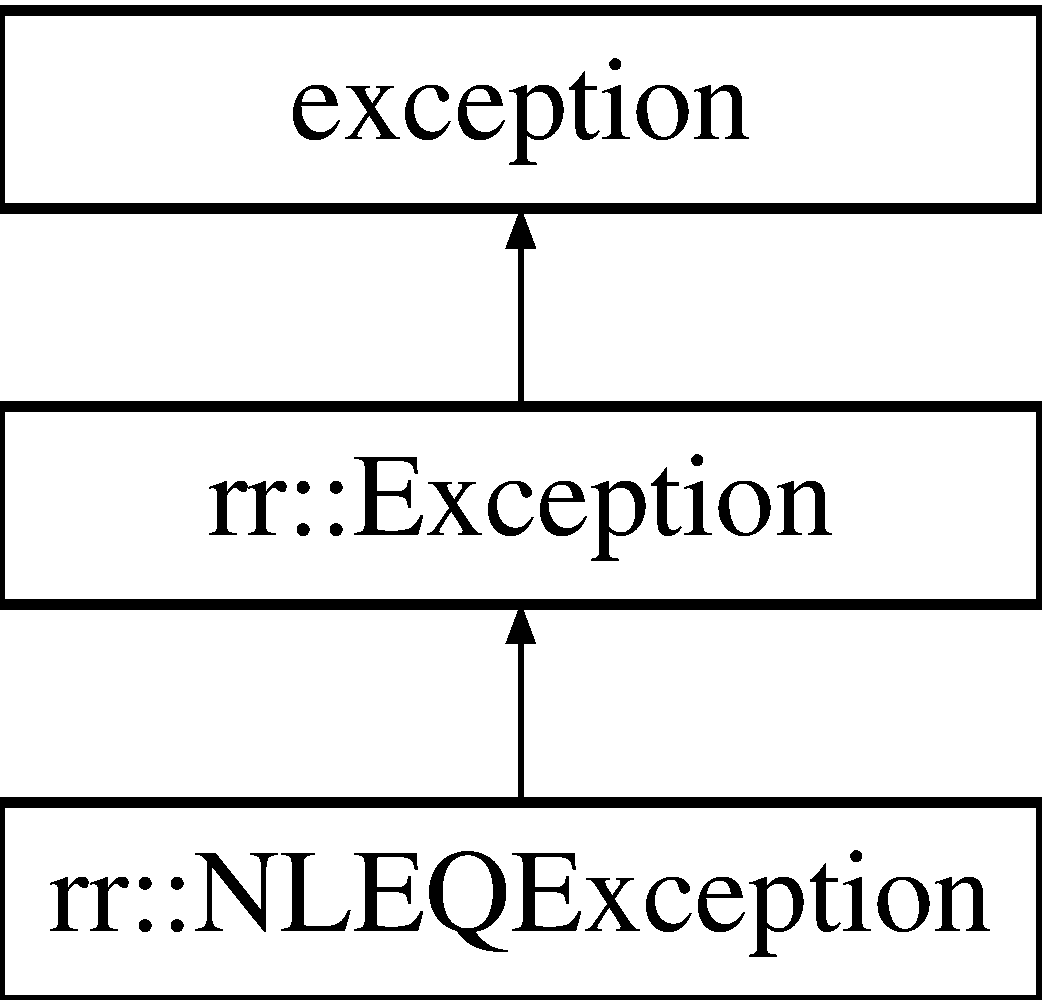
\includegraphics[height=3.000000cm]{classrr_1_1_n_l_e_q_exception}
\end{center}
\end{figure}
\subsection*{Public Member Functions}
\begin{DoxyCompactItemize}
\item 
\hypertarget{classrr_1_1_n_l_e_q_exception_a2ea10dbaba13749d37285c5000db4b28}{{\bfseries N\-L\-E\-Q\-Exception} (const string \&msg)}\label{classrr_1_1_n_l_e_q_exception_a2ea10dbaba13749d37285c5000db4b28}

\end{DoxyCompactItemize}
\subsection*{Additional Inherited Members}


The documentation for this class was generated from the following files\-:\begin{DoxyCompactItemize}
\item 
source/rr\-Exception.\-h\item 
source/rr\-Exception.\-cpp\end{DoxyCompactItemize}

\hypertarget{classrr_1_1_road_runner}{\section{rr\-:\-:Road\-Runner Class Reference}
\label{classrr_1_1_road_runner}\index{rr\-::\-Road\-Runner@{rr\-::\-Road\-Runner}}
}


{\ttfamily \#include $<$rr\-Road\-Runner.\-h$>$}

Inheritance diagram for rr\-:\-:Road\-Runner\-:\begin{figure}[H]
\begin{center}
\leavevmode
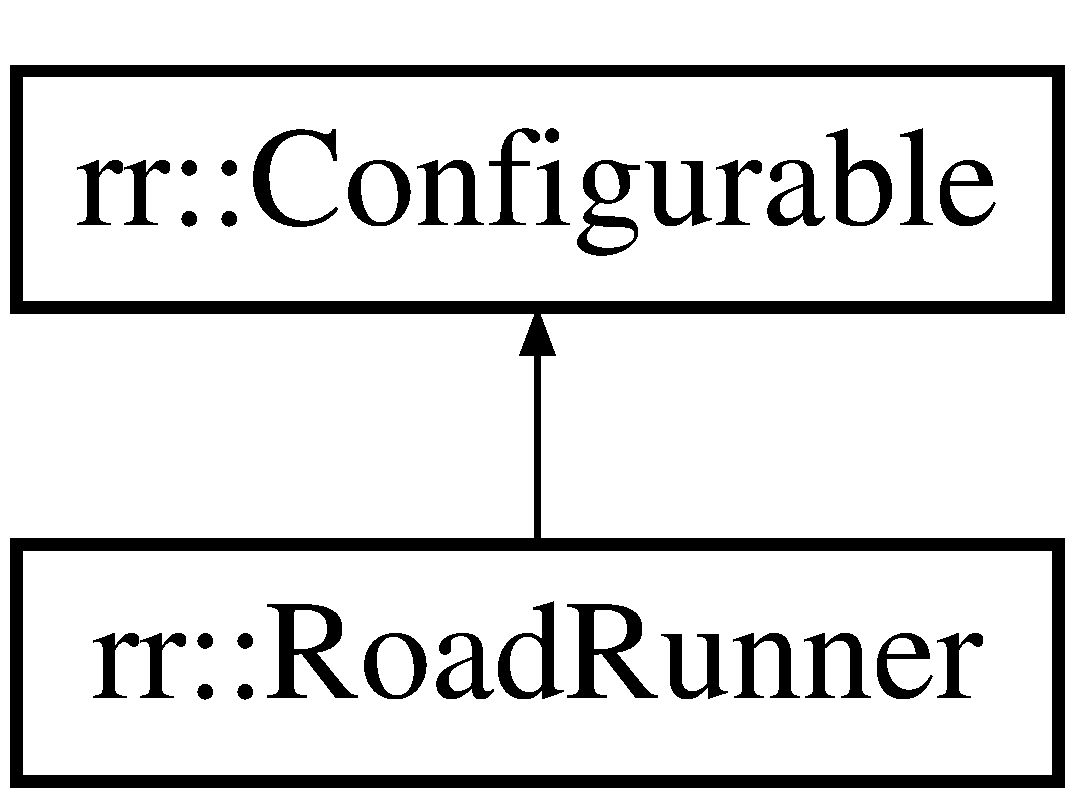
\includegraphics[height=2.000000cm]{classrr_1_1_road_runner}
\end{center}
\end{figure}
\subsection*{Public Member Functions}
\begin{DoxyCompactItemize}
\item 
\hyperlink{classrr_1_1_road_runner_a626f4bfe3accf4c6b0b61695b63ec481}{Road\-Runner} (const std\-::string \&compiler=\char`\"{}\char`\"{}, const std\-::string \&temp\-Dir=\char`\"{}\char`\"{}, const std\-::string \&support\-Code\-Dir=\char`\"{}\char`\"{})
\item 
virtual \hyperlink{classrr_1_1_road_runner_a102e7c27e29219ae56e48ffd607fd621}{$\sim$\-Road\-Runner} ()
\item 
int \hyperlink{classrr_1_1_road_runner_a6cc53f3668f94b3d88764e14b24bc87e}{get\-Instance\-I\-D} ()
\item 
int \hyperlink{classrr_1_1_road_runner_a4860f41d8552118f3c8c5d5fb6d999f6}{get\-Instance\-Count} ()
\item 
std\-::string \hyperlink{classrr_1_1_road_runner_a2b7022cadd857fa4fb3cb24703da608a}{get\-Info} ()
\item 
class \hyperlink{classrr_1_1_compiler}{Compiler} $\ast$ \hyperlink{classrr_1_1_road_runner_a329f2009c2688bbedc906c21c4b8b3ef}{get\-Compiler} ()
\item 
bool \hyperlink{classrr_1_1_road_runner_a4ce7d696fb39f5db0d9e4fa9f8f1192c}{set\-Compiler} (const std\-::string \&compiler)
\item 
\hyperlink{classrr_1_1_integrator}{Integrator} $\ast$ \hyperlink{classrr_1_1_road_runner_ac7ed0222daee67405616805b1bd02125}{get\-Integrator} ()
\item 
\hypertarget{classrr_1_1_road_runner_aecea2dbffc17d0322b00e18f126058b5}{bool {\bfseries is\-Model\-Loaded} ()}\label{classrr_1_1_road_runner_aecea2dbffc17d0322b00e18f126058b5}

\item 
std\-::string \hyperlink{classrr_1_1_road_runner_a9519f489ada956e35bd0b65e44e96cdd}{get\-Model\-Name} ()
\item 
\hypertarget{classrr_1_1_road_runner_ad19a3a222b25a0751ae8e968eec5eb45}{bool {\bfseries un\-Load\-Model} ()}\label{classrr_1_1_road_runner_ad19a3a222b25a0751ae8e968eec5eb45}

\item 
bool \hyperlink{classrr_1_1_road_runner_a61822e0ad53826249e04d72c3f45ab97}{set\-Temp\-File\-Folder} (const std\-::string \&folder)
\item 
std\-::string \hyperlink{classrr_1_1_road_runner_ad16dd282c20c5c144cab252f4e2752f1}{get\-Temp\-Folder} ()
\item 
double \hyperlink{classrr_1_1_road_runner_a27aedd28b2a2d5453200ca4a4a2bf4c0}{one\-Step} (double current\-Time, double step\-Size, bool \hyperlink{classrr_1_1_road_runner_ae4b0eaa39fd37737e5f5fd7f7741e06c}{reset}=true)
\item 
const \hyperlink{classrr_1_1_road_runner_data}{Road\-Runner\-Data} $\ast$ \hyperlink{classrr_1_1_road_runner_ae380c9a35cca24a7c35633bcd4c6836c}{simulate} (const \hyperlink{structrr_1_1_simulate_options}{Simulate\-Options} $\ast$options=0)
\item 
\hypertarget{classrr_1_1_road_runner_ab6f650b0473ff4b7432ff4fb8f2a9c61}{double {\bfseries get\-Value\-For\-Record} (const \hyperlink{classrr_1_1_selection_record}{Selection\-Record} \&record)}\label{classrr_1_1_road_runner_ab6f650b0473ff4b7432ff4fb8f2a9c61}

\item 
\hyperlink{classrr_1_1_road_runner_data}{Road\-Runner\-Data} $\ast$ \hyperlink{classrr_1_1_road_runner_aaf6508bdeb579b0eb79ec1cf23acc319}{get\-Simulation\-Result} ()
\item 
\hypertarget{classrr_1_1_road_runner_a8287ad042995275ccc20c92e9f4ccb9c}{bool {\bfseries set\-Simulate\-Options} (const \hyperlink{structrr_1_1_simulate_options}{Simulate\-Options} \&settings)}\label{classrr_1_1_road_runner_a8287ad042995275ccc20c92e9f4ccb9c}

\item 
const \hyperlink{structrr_1_1_simulate_options}{Simulate\-Options} \& \hyperlink{classrr_1_1_road_runner_ac5e47105d41a184299bbd4c9ec032257}{get\-Simulate\-Options} () const 
\item 
std\-::string \hyperlink{classrr_1_1_road_runner_ab46780863292ac487f9e32ebefd8e788}{get\-S\-B\-M\-L} ()
\item 
void \hyperlink{classrr_1_1_road_runner_ae4b0eaa39fd37737e5f5fd7f7741e06c}{reset} ()
\item 
void \hyperlink{classrr_1_1_road_runner_a57f1463dafcc61a90c3122a8fb37b08d}{change\-Initial\-Conditions} (const std\-::vector$<$ double $>$ \&ic)
\item 
\hyperlink{classrr_1_1_model_generator}{Model\-Generator} $\ast$ \hyperlink{classrr_1_1_road_runner_ada1e6bafd3e5dc03c5a04737f6922b0a}{get\-Model\-Generator} ()
\item 
\hyperlink{classrr_1_1_executable_model}{Executable\-Model} $\ast$ \hyperlink{classrr_1_1_road_runner_afa827d569de3c83dd286ac2aa25d1cf4}{get\-Model} ()
\item 
bool \hyperlink{classrr_1_1_road_runner_ae8b8feeff7bf6505b24410c67d3c50a3}{load\-S\-B\-M\-L\-From\-File} (const std\-::string \&file\-Name, const \hyperlink{structrr_1_1_load_s_b_m_l_options}{Load\-S\-B\-M\-L\-Options} $\ast$options=0)
\item 
bool \hyperlink{classrr_1_1_road_runner_a2ff55abccf558dee45752837ebddf2d5}{load\-S\-B\-M\-L} (const std\-::string \&sbml, const \hyperlink{structrr_1_1_load_s_b_m_l_options}{Load\-S\-B\-M\-L\-Options} $\ast$options=0)
\item 
std\-::vector$<$ double $>$ \hyperlink{classrr_1_1_road_runner_a7a0ea3394f25af5a84117c9ea8361dbd}{get\-Reaction\-Rates} ()
\item 
std\-::vector$<$ double $>$ \hyperlink{classrr_1_1_road_runner_a0bb915c515c4590da76e38a1346f0ed3}{get\-Rates\-Of\-Change} ()
\item 
std\-::vector$<$ std\-::string $>$ \hyperlink{classrr_1_1_road_runner_a3bcd761bfdad0571d290b6b23ea6f130}{get\-Reaction\-Ids} ()
\item 
virtual \-\_\-xml\-Node $\ast$ \hyperlink{classrr_1_1_road_runner_afd5401ecd63ac9dda2fe52f98066cb23}{create\-Config\-Node} ()
\item 
virtual void \hyperlink{classrr_1_1_road_runner_aac7ee8e64b2709d5d5a7e9b0cff8acc7}{load\-Config} (const \-\_\-xml\-Doc $\ast$doc)
\item 
std\-::string \hyperlink{classrr_1_1_road_runner_a1b92635414935e3d1d65fbac0d6871eb}{get\-Configuration\-X\-M\-L} ()
\item 
void \hyperlink{classrr_1_1_road_runner_a363c95863be438d85ac65b5db1b9bbe3}{set\-Configuration\-X\-M\-L} (const std\-::string \&xml)
\item 
\hypertarget{classrr_1_1_road_runner_a48965c4f1c455287f2e7ff1414da9d20}{void {\bfseries correct\-Max\-Step} ()}\label{classrr_1_1_road_runner_a48965c4f1c455287f2e7ff1414da9d20}

\item 
bool \hyperlink{classrr_1_1_road_runner_a27c852e00c2eae29242a2e4993d6e5d8}{set\-Value} (const std\-::string \&s\-Id, double value)
\item 
double \hyperlink{classrr_1_1_road_runner_aa8df587043e43c8d54e3f3293cecd767}{get\-Value} (const std\-::string \&s\-Id)
\item 
New\-Array\-List \hyperlink{classrr_1_1_road_runner_acb6ac6676114cf7658d39af85f19b0d3}{get\-Available\-Time\-Course\-Symbols} ()
\item 
std\-::vector$<$ std\-::string $>$ \hyperlink{classrr_1_1_road_runner_a59e81eb385e66c02671df6c9cd30297b}{get\-Time\-Course\-Selection\-List} ()
\item 
\hypertarget{classrr_1_1_road_runner_a32c932092a000311b23001c6fe16a5c0}{void {\bfseries set\-Time\-Course\-Selection\-List} (const std\-::string \&List)}\label{classrr_1_1_road_runner_a32c932092a000311b23001c6fe16a5c0}

\item 
\hypertarget{classrr_1_1_road_runner_a7ef87de1f436bf2317f2930cf4a3d85a}{void {\bfseries set\-Time\-Course\-Selection\-List} (const std\-::vector$<$ std\-::string $>$ \&new\-Selection\-List)}\label{classrr_1_1_road_runner_a7ef87de1f436bf2317f2930cf4a3d85a}

\item 
double \hyperlink{classrr_1_1_road_runner_a53b8b7426d67ec2c15ed2b19785253e4}{steady\-State} ()
\item 
ls\-::\-Double\-Matrix \hyperlink{classrr_1_1_road_runner_af51e91db7ddc73786511271278f6c096}{get\-Full\-Jacobian} ()
\item 
\hypertarget{classrr_1_1_road_runner_a050e99e35e27a60e795825fdeb58c21d}{ls\-::\-Double\-Matrix {\bfseries get\-Full\-Reordered\-Jacobian} ()}\label{classrr_1_1_road_runner_a050e99e35e27a60e795825fdeb58c21d}

\item 
ls\-::\-Double\-Matrix \hyperlink{classrr_1_1_road_runner_a94471743a00815af37b0e598208605a5}{get\-Reduced\-Jacobian} ()
\item 
ls\-::\-Double\-Matrix \hyperlink{classrr_1_1_road_runner_af2ffe24f0f93699601b92d79ec291aa2}{get\-Eigenvalues} ()
\item 
\hypertarget{classrr_1_1_road_runner_aaba61d3b9bb97c7a8ac5262cb731da7f}{std\-::vector$<$ Complex $>$ {\bfseries get\-Eigenvalues\-Cpx} ()}\label{classrr_1_1_road_runner_aaba61d3b9bb97c7a8ac5262cb731da7f}

\item 
\hypertarget{classrr_1_1_road_runner_a7dc49b36a1511224cf0d31cf701c79fc}{ls\-::\-Double\-Matrix $\ast$ {\bfseries get\-Link\-Matrix} ()}\label{classrr_1_1_road_runner_a7dc49b36a1511224cf0d31cf701c79fc}

\item 
\hypertarget{classrr_1_1_road_runner_ab4a40675344ec66d4756cea8dd0bb655}{ls\-::\-Double\-Matrix $\ast$ {\bfseries get\-Nr\-Matrix} ()}\label{classrr_1_1_road_runner_ab4a40675344ec66d4756cea8dd0bb655}

\item 
\hypertarget{classrr_1_1_road_runner_aa973f431635e09699b548ccbc584588b}{ls\-::\-Double\-Matrix $\ast$ {\bfseries get\-L0\-Matrix} ()}\label{classrr_1_1_road_runner_aa973f431635e09699b548ccbc584588b}

\item 
\hypertarget{classrr_1_1_road_runner_ae14f16f6d85d11d051b58643961cbc78}{ls\-::\-Double\-Matrix {\bfseries get\-Stoichiometry\-Matrix} ()}\label{classrr_1_1_road_runner_ae14f16f6d85d11d051b58643961cbc78}

\item 
\hypertarget{classrr_1_1_road_runner_a44dd3263687e6aa2900462ab29672ca3}{ls\-::\-Double\-Matrix {\bfseries get\-Reordered\-Stoichiometry\-Matrix} ()}\label{classrr_1_1_road_runner_a44dd3263687e6aa2900462ab29672ca3}

\item 
\hypertarget{classrr_1_1_road_runner_a75b8513f8024222edd4f31fbc7da9b24}{ls\-::\-Double\-Matrix {\bfseries get\-Fully\-Reordered\-Stoichiometry\-Matrix} ()}\label{classrr_1_1_road_runner_a75b8513f8024222edd4f31fbc7da9b24}

\item 
\hypertarget{classrr_1_1_road_runner_a6fa2cd47bfc3c40d74e775029dab6d4e}{ls\-::\-Double\-Matrix {\bfseries get\-Conservation\-Matrix} ()}\label{classrr_1_1_road_runner_a6fa2cd47bfc3c40d74e775029dab6d4e}

\item 
\hypertarget{classrr_1_1_road_runner_a1926e6503e60ebcc37ae339b597a25a3}{ls\-::\-Double\-Matrix {\bfseries get\-Unscaled\-Concentration\-Control\-Coefficient\-Matrix} ()}\label{classrr_1_1_road_runner_a1926e6503e60ebcc37ae339b597a25a3}

\item 
\hypertarget{classrr_1_1_road_runner_a1ed7c5519b10fea5a9e19eaab5f1fda7}{ls\-::\-Double\-Matrix {\bfseries get\-Scaled\-Concentration\-Control\-Coefficient\-Matrix} ()}\label{classrr_1_1_road_runner_a1ed7c5519b10fea5a9e19eaab5f1fda7}

\item 
\hypertarget{classrr_1_1_road_runner_ae8f9e20c1586d0a95f538d5c1bf301f2}{ls\-::\-Double\-Matrix {\bfseries get\-Unscaled\-Flux\-Control\-Coefficient\-Matrix} ()}\label{classrr_1_1_road_runner_ae8f9e20c1586d0a95f538d5c1bf301f2}

\item 
\hypertarget{classrr_1_1_road_runner_abe4dde40c03d296f2ed45db095779c28}{ls\-::\-Double\-Matrix {\bfseries get\-Scaled\-Flux\-Control\-Coefficient\-Matrix} ()}\label{classrr_1_1_road_runner_abe4dde40c03d296f2ed45db095779c28}

\item 
\hypertarget{classrr_1_1_road_runner_a78708a8b3088ada0b5d7b2630a24904e}{int {\bfseries get\-Number\-Of\-Dependent\-Species} ()}\label{classrr_1_1_road_runner_a78708a8b3088ada0b5d7b2630a24904e}

\item 
\hypertarget{classrr_1_1_road_runner_a0cbcdf248d716058325e50adf9239d4d}{int {\bfseries get\-Number\-Of\-Independent\-Species} ()}\label{classrr_1_1_road_runner_a0cbcdf248d716058325e50adf9239d4d}

\item 
New\-Array\-List \hyperlink{classrr_1_1_road_runner_ad8c4fb1e371aa0aae7d526852d735cca}{get\-Unscaled\-Flux\-Control\-Coefficient\-Ids} ()
\item 
New\-Array\-List \hyperlink{classrr_1_1_road_runner_aa86c7d1f1e4ea63a6682057012798ba4}{get\-Flux\-Control\-Coefficient\-Ids} ()
\item 
New\-Array\-List \hyperlink{classrr_1_1_road_runner_a5f1ec08327987f8db240384b7dacb612}{get\-Unscaled\-Concentration\-Control\-Coefficient\-Ids} ()
\item 
New\-Array\-List \hyperlink{classrr_1_1_road_runner_aa5e73ec2cffc8af01adef44f95991754}{get\-Concentration\-Control\-Coefficient\-Ids} ()
\item 
New\-Array\-List \hyperlink{classrr_1_1_road_runner_ae718da692d33600644a9017d1d2b9947}{get\-Elasticity\-Coefficient\-Ids} ()
\item 
New\-Array\-List \hyperlink{classrr_1_1_road_runner_adad3fdd2e30911720d1c5719748f8f13}{get\-Unscaled\-Elasticity\-Coefficient\-Ids} ()
\item 
std\-::vector$<$ std\-::string $>$ \hyperlink{classrr_1_1_road_runner_afef1779a575df9d4905d281e485795f1}{get\-Eigenvalue\-Ids} ()
\item 
\hypertarget{classrr_1_1_road_runner_a683644a637a9cad0cb127c8e70734494}{std\-::vector$<$ std\-::string $>$ {\bfseries get\-Steady\-State\-Selection\-List} ()}\label{classrr_1_1_road_runner_a683644a637a9cad0cb127c8e70734494}

\item 
\hypertarget{classrr_1_1_road_runner_a633566f910a2137f8085df12a16d3d9a}{void {\bfseries set\-Steady\-State\-Selection\-List} (const std\-::vector$<$ std\-::string $>$ \&new\-Selection\-List)}\label{classrr_1_1_road_runner_a633566f910a2137f8085df12a16d3d9a}

\item 
\hypertarget{classrr_1_1_road_runner_a0738b1cb3659a2d7d027f7653facf70c}{double {\bfseries compute\-Steady\-State\-Value} (const \hyperlink{classrr_1_1_selection_record}{Selection\-Record} \&record)}\label{classrr_1_1_road_runner_a0738b1cb3659a2d7d027f7653facf70c}

\item 
std\-::vector$<$ double $>$ \hyperlink{classrr_1_1_road_runner_ab8cc67d7107205fe8e5f253bccbb208b}{compute\-Steady\-State\-Values} ()
\item 
std\-::vector$<$ double $>$ \hyperlink{classrr_1_1_road_runner_a9f08b6d6151a3635a2d4618f8c700b53}{compute\-Steady\-State\-Values} (const std\-::vector$<$ \hyperlink{classrr_1_1_selection_record}{Selection\-Record} $>$ \&selection, bool compute\-Steady\-State)
\item 
\hypertarget{classrr_1_1_road_runner_aab81568c3bf4b73f49fd7a746f8bf0c8}{double {\bfseries compute\-Steady\-State\-Value} (const std\-::string \&s\-Id)}\label{classrr_1_1_road_runner_aab81568c3bf4b73f49fd7a746f8bf0c8}

\item 
std\-::vector$<$ double $>$ \hyperlink{classrr_1_1_road_runner_a9c98b4f3d57c4935b744d8cd831d4a61}{get\-Selected\-Values} ()
\item 
void \hyperlink{classrr_1_1_road_runner_a1e7fa0ce52890140e95014dc452ef1a3}{set\-Conservation\-Analysis} (bool value)
\item 
bool \hyperlink{classrr_1_1_road_runner_a51edc11ea3158972f7109dd73a084286}{get\-Conservation\-Analysis} ()
\item 
std\-::string \hyperlink{classrr_1_1_road_runner_a2a2507cc2964f8aef0d200c5841bc218}{write\-S\-B\-M\-L} ()
\item 
\hypertarget{classrr_1_1_road_runner_a0aeef3b4db855e2cd6e901372c9082f2}{int {\bfseries get\-Number\-Of\-Reactions} ()}\label{classrr_1_1_road_runner_a0aeef3b4db855e2cd6e901372c9082f2}

\item 
\hypertarget{classrr_1_1_road_runner_a9284f10d515b8ef441473b5c14f5920e}{double {\bfseries get\-Reaction\-Rate} (const int \&index)}\label{classrr_1_1_road_runner_a9284f10d515b8ef441473b5c14f5920e}

\item 
double \hyperlink{classrr_1_1_road_runner_a67736588f72a8fb4f429368716acda93}{get\-Rate\-Of\-Change} (const int \&index)
\item 
\hypertarget{classrr_1_1_road_runner_a5d9266988c75e838d2a2c020a35304b2}{std\-::vector$<$ std\-::string $>$ {\bfseries get\-Rate\-Of\-Change\-Ids} ()}\label{classrr_1_1_road_runner_a5d9266988c75e838d2a2c020a35304b2}

\item 
\hypertarget{classrr_1_1_road_runner_af7cf29c009117099cc41b46b3e2df443}{std\-::vector$<$ double $>$ {\bfseries get\-Rates\-Of\-Change\-Ex} (const std\-::vector$<$ double $>$ \&values)}\label{classrr_1_1_road_runner_af7cf29c009117099cc41b46b3e2df443}

\item 
\hypertarget{classrr_1_1_road_runner_aac792c2a8c0a6f47cf987f64bbf0ac4f}{std\-::vector$<$ double $>$ {\bfseries get\-Reaction\-Rates\-Ex} (const std\-::vector$<$ double $>$ \&values)}\label{classrr_1_1_road_runner_aac792c2a8c0a6f47cf987f64bbf0ac4f}

\item 
\hypertarget{classrr_1_1_road_runner_a158be8a09cc4bc786c7441a72748bcd0}{std\-::vector$<$ std\-::string $>$ {\bfseries get\-Conserved\-Sum\-Ids} ()}\label{classrr_1_1_road_runner_a158be8a09cc4bc786c7441a72748bcd0}

\item 
\hypertarget{classrr_1_1_road_runner_a87974f2dd5fcb693d0dc519f645a420a}{std\-::vector$<$ double $>$ {\bfseries get\-Conserved\-Sums} ()}\label{classrr_1_1_road_runner_a87974f2dd5fcb693d0dc519f645a420a}

\item 
\hypertarget{classrr_1_1_road_runner_a2f26307521e9930a85ed5c44bae67cfa}{int {\bfseries get\-Number\-Of\-Compartments} ()}\label{classrr_1_1_road_runner_a2f26307521e9930a85ed5c44bae67cfa}

\item 
void \hyperlink{classrr_1_1_road_runner_a01dbe5358bd652891be6209260523cb6}{set\-Compartment\-By\-Index} (const int \&index, const double \&value)
\item 
double \hyperlink{classrr_1_1_road_runner_a14b51ebe111fd7292dbca21a2749125b}{get\-Compartment\-By\-Index} (const int \&index)
\item 
std\-::vector$<$ std\-::string $>$ \hyperlink{classrr_1_1_road_runner_af5dfe0456563a2f364762ac9e839f273}{get\-Compartment\-Ids} ()
\item 
int \hyperlink{classrr_1_1_road_runner_a54a9d80927c998e0981a2deac0671758}{get\-Number\-Of\-Boundary\-Species} ()
\item 
void \hyperlink{classrr_1_1_road_runner_af8d2ff8ebf2c85f918cc2888ac68f479}{set\-Boundary\-Species\-By\-Index} (const int \&index, const double \&value)
\item 
double \hyperlink{classrr_1_1_road_runner_afc7498e1fe7098233c87f4427e74509b}{get\-Boundary\-Species\-By\-Index} (const int \&index)
\item 
std\-::vector$<$ double $>$ \hyperlink{classrr_1_1_road_runner_aa8b3a8ad7d52eb86a9a6b5970510e569}{get\-Boundary\-Species\-Concentrations} ()
\item 
void \hyperlink{classrr_1_1_road_runner_a42a995530149829e8deda1a18419a864}{set\-Boundary\-Species\-Concentrations} (const std\-::vector$<$ double $>$ \&values)
\item 
std\-::vector$<$ std\-::string $>$ \hyperlink{classrr_1_1_road_runner_afb363e6354cc06772219f3f59b591320}{get\-Boundary\-Species\-Ids} ()
\item 
int \hyperlink{classrr_1_1_road_runner_af2467ad14443e89ac9a1ed98481093c3}{get\-Number\-Of\-Floating\-Species} ()
\item 
\hypertarget{classrr_1_1_road_runner_ab06b478ffc51b1c0bad9926ae1840ab9}{void {\bfseries set\-Floating\-Species\-By\-Index} (const int \&index, const double \&value)}\label{classrr_1_1_road_runner_ab06b478ffc51b1c0bad9926ae1840ab9}

\item 
\hypertarget{classrr_1_1_road_runner_a842015aa1d5a024a0d4a96443cb3977e}{double {\bfseries get\-Floating\-Species\-Initial\-Concentration\-By\-Index} (const int \&index)}\label{classrr_1_1_road_runner_a842015aa1d5a024a0d4a96443cb3977e}

\item 
\hypertarget{classrr_1_1_road_runner_a6c15d6020db73f2cba5cc048360222cd}{double {\bfseries get\-Floating\-Species\-By\-Index} (const int \&index)}\label{classrr_1_1_road_runner_a6c15d6020db73f2cba5cc048360222cd}

\item 
\hypertarget{classrr_1_1_road_runner_a8bfb3b2b523a9448617b99568e4af757}{std\-::vector$<$ double $>$ {\bfseries get\-Floating\-Species\-Concentrations} ()}\label{classrr_1_1_road_runner_a8bfb3b2b523a9448617b99568e4af757}

\item 
\hypertarget{classrr_1_1_road_runner_ae123a31ab81aa07d8e67f385608fb8da}{std\-::vector$<$ double $>$ {\bfseries get\-Floating\-Species\-Initial\-Concentrations} ()}\label{classrr_1_1_road_runner_ae123a31ab81aa07d8e67f385608fb8da}

\item 
\hypertarget{classrr_1_1_road_runner_a5e1dcd14759e468e510a298f61b267de}{void {\bfseries set\-Floating\-Species\-Concentrations} (const std\-::vector$<$ double $>$ \&values)}\label{classrr_1_1_road_runner_a5e1dcd14759e468e510a298f61b267de}

\item 
\hypertarget{classrr_1_1_road_runner_a08176e93872548591ce96b2f9c20dc74}{void {\bfseries set\-Floating\-Species\-Initial\-Concentration\-By\-Index} (const int \&index, const double \&value)}\label{classrr_1_1_road_runner_a08176e93872548591ce96b2f9c20dc74}

\item 
\hypertarget{classrr_1_1_road_runner_a3c85d3178f85ec302f1dd8f13fb87aa8}{void {\bfseries set\-Floating\-Species\-Initial\-Concentrations} (const std\-::vector$<$ double $>$ \&values)}\label{classrr_1_1_road_runner_a3c85d3178f85ec302f1dd8f13fb87aa8}

\item 
\hypertarget{classrr_1_1_road_runner_a40a8147fbf0732416b0f0cbdf405158c}{std\-::vector$<$ std\-::string $>$ {\bfseries get\-Floating\-Species\-Ids} ()}\label{classrr_1_1_road_runner_a40a8147fbf0732416b0f0cbdf405158c}

\item 
\hypertarget{classrr_1_1_road_runner_a60d71f2afe4aaedac4226fb3d4093a52}{std\-::vector$<$ std\-::string $>$ {\bfseries get\-Floating\-Species\-Initial\-Condition\-Ids} ()}\label{classrr_1_1_road_runner_a60d71f2afe4aaedac4226fb3d4093a52}

\item 
\hypertarget{classrr_1_1_road_runner_a2063359eac303ac7b18ea275bdc78372}{std\-::vector$<$ std\-::string $>$ {\bfseries get\-Floating\-Species\-Amount\-Ids} ()}\label{classrr_1_1_road_runner_a2063359eac303ac7b18ea275bdc78372}

\item 
int \hyperlink{classrr_1_1_road_runner_ae89a7ec21d11f3a6a8f23b94f8d41044}{get\-Number\-Of\-Global\-Parameters} ()
\item 
void \hyperlink{classrr_1_1_road_runner_aa90f680c2d8e3c1dbd67c90de015338c}{set\-Global\-Parameter\-By\-Index} (const int index, const double value)
\item 
double \hyperlink{classrr_1_1_road_runner_a241c4374d564427ef61df52862136574}{get\-Global\-Parameter\-By\-Index} (const int \&index)
\item 
std\-::vector$<$ double $>$ \hyperlink{classrr_1_1_road_runner_ad3c1380f0ac290590534899d4c9478a4}{get\-Global\-Parameter\-Values} ()
\item 
std\-::vector$<$ std\-::string $>$ \hyperlink{classrr_1_1_road_runner_a5344345156070f4bab82d9b81b7050de}{get\-Global\-Parameter\-Ids} ()
\item 
void \hyperlink{classrr_1_1_road_runner_ad3f4b6ef217424cb9b12c798dfd1129c}{eval\-Model} ()
\item 
double \hyperlink{classrr_1_1_road_runner_a7df50d5a0fa7265b62af24a2e996b6e0}{getu\-C\-C} (const std\-::string \&variable\-Name, const std\-::string \&parameter\-Name)
\item 
double \hyperlink{classrr_1_1_road_runner_a3d2c1d4727f38714ce6575a70d789429}{get\-C\-C} (const std\-::string \&variable\-Name, const std\-::string \&parameter\-Name)
\item 
double \hyperlink{classrr_1_1_road_runner_ad1a582f68475ad9e923dd23b12397d86}{getu\-E\-E} (const std\-::string \&reaction\-Name, const std\-::string \&parameter\-Name)
\item 
double \hyperlink{classrr_1_1_road_runner_a6957a9119e32959e4bbd47107a22f8a5}{getu\-E\-E} (const std\-::string \&reaction\-Name, const std\-::string \&parameter\-Name, bool compute\-Steadystate)
\item 
double \hyperlink{classrr_1_1_road_runner_a4faad67b12aaf15212f7c57697556d61}{get\-E\-E} (const std\-::string \&reaction\-Name, const std\-::string \&parameter\-Name)
\item 
double \hyperlink{classrr_1_1_road_runner_a54d7fece5e6ac6fcba4d113f62aff1e4}{get\-E\-E} (const std\-::string \&reaction\-Name, const std\-::string \&parameter\-Name, bool compute\-Steady\-State)
\item 
ls\-::\-Double\-Matrix \hyperlink{classrr_1_1_road_runner_a60d096cd0738a337899ae6c6109c178e}{get\-Unscaled\-Elasticity\-Matrix} ()
\item 
ls\-::\-Double\-Matrix \hyperlink{classrr_1_1_road_runner_a08b4ba485aeefc3275c49d393a18a2b1}{get\-Scaled\-Reordered\-Elasticity\-Matrix} ()
\item 
double \hyperlink{classrr_1_1_road_runner_a6a388eb7c0f64e215490fa606f458770}{get\-Scaled\-Floating\-Species\-Elasticity} (const std\-::string \&reaction\-Name, const std\-::string \&species\-Name)
\item 
double \hyperlink{classrr_1_1_road_runner_a5856b94d04fadfb190b407b126382503}{get\-Unscaled\-Species\-Elasticity} (int reaction\-Id, int species\-Index)
\end{DoxyCompactItemize}
\subsection*{Static Public Member Functions}
\begin{DoxyCompactItemize}
\item 
static std\-::string \hyperlink{classrr_1_1_road_runner_ab04e0b440a74f7d49f55751b346f4212}{get\-Param\-Promoted\-S\-B\-M\-L} (const std\-::string \&s\-Arg)
\item 
\hypertarget{classrr_1_1_road_runner_aa054cc8411c416aff41d61c8639ee6bd}{static std\-::string {\bfseries getlib\-S\-B\-M\-L\-Version} ()}\label{classrr_1_1_road_runner_aa054cc8411c416aff41d61c8639ee6bd}

\item 
static std\-::string \hyperlink{classrr_1_1_road_runner_a248d078936a41d47c8de44ac829389f4}{get\-Version} ()
\item 
static std\-::string \hyperlink{classrr_1_1_road_runner_afdb1fa322ff0f3d53e33e30558bbe478}{get\-Extended\-Version\-Info} ()
\item 
static std\-::string \hyperlink{classrr_1_1_road_runner_a4b773957d863f152b5744904e5229ca6}{get\-Copyright} ()
\end{DoxyCompactItemize}


\subsection{Detailed Description}
The main \hyperlink{classrr_1_1_road_runner}{Road\-Runner} class.

The \hyperlink{classrr_1_1_road_runner}{Road\-Runner} class is responsible for loading and simulating S\-B\-M\-L models.

Memory\-Managment\-: Any pointer returned by a get... method is owned by the \hyperlink{classrr_1_1_road_runner}{Road\-Runner} object and does N\-O\-T have to be deleted. 

\subsection{Constructor \& Destructor Documentation}
\hypertarget{classrr_1_1_road_runner_a626f4bfe3accf4c6b0b61695b63ec481}{\index{rr\-::\-Road\-Runner@{rr\-::\-Road\-Runner}!Road\-Runner@{Road\-Runner}}
\index{Road\-Runner@{Road\-Runner}!rr::RoadRunner@{rr\-::\-Road\-Runner}}
\subsubsection[{Road\-Runner}]{\setlength{\rightskip}{0pt plus 5cm}rr\-::\-Road\-Runner\-::\-Road\-Runner (
\begin{DoxyParamCaption}
\item[{const std\-::string \&}]{compiler = {\ttfamily \char`\"{}\char`\"{}}, }
\item[{const std\-::string \&}]{temp\-Dir = {\ttfamily \char`\"{}\char`\"{}}, }
\item[{const std\-::string \&}]{support\-Code\-Dir = {\ttfamily \char`\"{}\char`\"{}}}
\end{DoxyParamCaption}
)}}\label{classrr_1_1_road_runner_a626f4bfe3accf4c6b0b61695b63ec481}
All three of the \hyperlink{classrr_1_1_road_runner}{Road\-Runner} options default to the empty string, in this case, the default values are used.


\begin{DoxyParams}{Parameters}
{\em compiler,\-:} & If L\-L\-V\-M build is enabled, the compiler defaults to L\-L\-V\-M. \\
\hline
{\em temp\-Dir,\-:} & If the old external C compiler is used, this is the where the C files are written to. \\
\hline
{\em support\-Code\-Dir,\-:} & If the old external C compiler is used, this is the location where roadrunner C include files are. \\
\hline
\end{DoxyParams}
\hypertarget{classrr_1_1_road_runner_a102e7c27e29219ae56e48ffd607fd621}{\index{rr\-::\-Road\-Runner@{rr\-::\-Road\-Runner}!$\sim$\-Road\-Runner@{$\sim$\-Road\-Runner}}
\index{$\sim$\-Road\-Runner@{$\sim$\-Road\-Runner}!rr::RoadRunner@{rr\-::\-Road\-Runner}}
\subsubsection[{$\sim$\-Road\-Runner}]{\setlength{\rightskip}{0pt plus 5cm}rr\-::\-Road\-Runner\-::$\sim$\-Road\-Runner (
\begin{DoxyParamCaption}
{}
\end{DoxyParamCaption}
)\hspace{0.3cm}{\ttfamily [virtual]}}}\label{classrr_1_1_road_runner_a102e7c27e29219ae56e48ffd607fd621}
free any memory this class allocated 

\subsection{Member Function Documentation}
\hypertarget{classrr_1_1_road_runner_a57f1463dafcc61a90c3122a8fb37b08d}{\index{rr\-::\-Road\-Runner@{rr\-::\-Road\-Runner}!change\-Initial\-Conditions@{change\-Initial\-Conditions}}
\index{change\-Initial\-Conditions@{change\-Initial\-Conditions}!rr::RoadRunner@{rr\-::\-Road\-Runner}}
\subsubsection[{change\-Initial\-Conditions}]{\setlength{\rightskip}{0pt plus 5cm}void rr\-::\-Road\-Runner\-::change\-Initial\-Conditions (
\begin{DoxyParamCaption}
\item[{const std\-::vector$<$ double $>$ \&}]{ic}
\end{DoxyParamCaption}
)}}\label{classrr_1_1_road_runner_a57f1463dafcc61a90c3122a8fb37b08d}
set the floating species initial concentrations.

equivalent to \hyperlink{classrr_1_1_executable_model_a217c61819d9b029c5928ace53b805e89}{Executable\-Model\-::reset}, then \hyperlink{classrr_1_1_executable_model_a42853a01cc2fae3b4a064d820ebacfaf}{Executable\-Model\-::set\-Floating\-Species\-Concentrations}

\begin{DoxyRefDesc}{Deprecated}
\item[\hyperlink{deprecated__deprecated000002}{Deprecated}]\end{DoxyRefDesc}
\hypertarget{classrr_1_1_road_runner_ab8cc67d7107205fe8e5f253bccbb208b}{\index{rr\-::\-Road\-Runner@{rr\-::\-Road\-Runner}!compute\-Steady\-State\-Values@{compute\-Steady\-State\-Values}}
\index{compute\-Steady\-State\-Values@{compute\-Steady\-State\-Values}!rr::RoadRunner@{rr\-::\-Road\-Runner}}
\subsubsection[{compute\-Steady\-State\-Values}]{\setlength{\rightskip}{0pt plus 5cm}vector$<$ double $>$ rr\-::\-Road\-Runner\-::compute\-Steady\-State\-Values (
\begin{DoxyParamCaption}
{}
\end{DoxyParamCaption}
)}}\label{classrr_1_1_road_runner_ab8cc67d7107205fe8e5f253bccbb208b}
returns the value of the given steady state identifier. \hypertarget{classrr_1_1_road_runner_a9f08b6d6151a3635a2d4618f8c700b53}{\index{rr\-::\-Road\-Runner@{rr\-::\-Road\-Runner}!compute\-Steady\-State\-Values@{compute\-Steady\-State\-Values}}
\index{compute\-Steady\-State\-Values@{compute\-Steady\-State\-Values}!rr::RoadRunner@{rr\-::\-Road\-Runner}}
\subsubsection[{compute\-Steady\-State\-Values}]{\setlength{\rightskip}{0pt plus 5cm}std\-::vector$<$double$>$ rr\-::\-Road\-Runner\-::compute\-Steady\-State\-Values (
\begin{DoxyParamCaption}
\item[{const std\-::vector$<$ {\bf Selection\-Record} $>$ \&}]{selection, }
\item[{bool}]{compute\-Steady\-State}
\end{DoxyParamCaption}
)}}\label{classrr_1_1_road_runner_a9f08b6d6151a3635a2d4618f8c700b53}
optionally compute the steady state and return a vector of the steady state values.


\begin{DoxyParams}{Parameters}
{\em selection,\-:} & the list of selections to get values for. \\
\hline
{\em compute\-Steady\-State,\-:} & compute the steady state. \\
\hline
\end{DoxyParams}
\hypertarget{classrr_1_1_road_runner_afd5401ecd63ac9dda2fe52f98066cb23}{\index{rr\-::\-Road\-Runner@{rr\-::\-Road\-Runner}!create\-Config\-Node@{create\-Config\-Node}}
\index{create\-Config\-Node@{create\-Config\-Node}!rr::RoadRunner@{rr\-::\-Road\-Runner}}
\subsubsection[{create\-Config\-Node}]{\setlength{\rightskip}{0pt plus 5cm}\-\_\-xml\-Node $\ast$ rr\-::\-Road\-Runner\-::create\-Config\-Node (
\begin{DoxyParamCaption}
{}
\end{DoxyParamCaption}
)\hspace{0.3cm}{\ttfamily [virtual]}}}\label{classrr_1_1_road_runner_afd5401ecd63ac9dda2fe52f98066cb23}
creates a new xml element that represent the current state of this \hyperlink{classrr_1_1_configurable}{Configurable} object and all if its child objects.

This node needs to be consumed by \hyperlink{classrr_1_1_configurable_a326b7f6db697fb213908234b0135b93b}{Configurable\-::xml\-From\-Config\-Node} 

Implements \hyperlink{classrr_1_1_configurable_af1eeec76874dccc105e70f5fd2255df3}{rr\-::\-Configurable}.

\hypertarget{classrr_1_1_road_runner_ad3f4b6ef217424cb9b12c798dfd1129c}{\index{rr\-::\-Road\-Runner@{rr\-::\-Road\-Runner}!eval\-Model@{eval\-Model}}
\index{eval\-Model@{eval\-Model}!rr::RoadRunner@{rr\-::\-Road\-Runner}}
\subsubsection[{eval\-Model}]{\setlength{\rightskip}{0pt plus 5cm}void rr\-::\-Road\-Runner\-::eval\-Model (
\begin{DoxyParamCaption}
{}
\end{DoxyParamCaption}
)}}\label{classrr_1_1_road_runner_ad3f4b6ef217424cb9b12c798dfd1129c}
The C back end requires this to be called to update model variables if anyting is changes. Does nothing in L\-L\-V\-M back end as everything is automatically handled with lazy evaluation. \hypertarget{classrr_1_1_road_runner_acb6ac6676114cf7658d39af85f19b0d3}{\index{rr\-::\-Road\-Runner@{rr\-::\-Road\-Runner}!get\-Available\-Time\-Course\-Symbols@{get\-Available\-Time\-Course\-Symbols}}
\index{get\-Available\-Time\-Course\-Symbols@{get\-Available\-Time\-Course\-Symbols}!rr::RoadRunner@{rr\-::\-Road\-Runner}}
\subsubsection[{get\-Available\-Time\-Course\-Symbols}]{\setlength{\rightskip}{0pt plus 5cm}New\-Array\-List rr\-::\-Road\-Runner\-::get\-Available\-Time\-Course\-Symbols (
\begin{DoxyParamCaption}
{}
\end{DoxyParamCaption}
)}}\label{classrr_1_1_road_runner_acb6ac6676114cf7658d39af85f19b0d3}
\begin{DoxyRefDesc}{Deprecated}
\item[\hyperlink{deprecated__deprecated000005}{Deprecated}]\end{DoxyRefDesc}
\hypertarget{classrr_1_1_road_runner_afc7498e1fe7098233c87f4427e74509b}{\index{rr\-::\-Road\-Runner@{rr\-::\-Road\-Runner}!get\-Boundary\-Species\-By\-Index@{get\-Boundary\-Species\-By\-Index}}
\index{get\-Boundary\-Species\-By\-Index@{get\-Boundary\-Species\-By\-Index}!rr::RoadRunner@{rr\-::\-Road\-Runner}}
\subsubsection[{get\-Boundary\-Species\-By\-Index}]{\setlength{\rightskip}{0pt plus 5cm}double rr\-::\-Road\-Runner\-::get\-Boundary\-Species\-By\-Index (
\begin{DoxyParamCaption}
\item[{const int \&}]{index}
\end{DoxyParamCaption}
)}}\label{classrr_1_1_road_runner_afc7498e1fe7098233c87f4427e74509b}
\begin{DoxyRefDesc}{Deprecated}
\item[\hyperlink{deprecated__deprecated000017}{Deprecated}], use \hyperlink{classrr_1_1_executable_model_a20e84c758da51167874aee3c66d8f576}{Executable\-Model\-::get\-Boundary\-Species\-Concentrations} \end{DoxyRefDesc}
\hypertarget{classrr_1_1_road_runner_aa8b3a8ad7d52eb86a9a6b5970510e569}{\index{rr\-::\-Road\-Runner@{rr\-::\-Road\-Runner}!get\-Boundary\-Species\-Concentrations@{get\-Boundary\-Species\-Concentrations}}
\index{get\-Boundary\-Species\-Concentrations@{get\-Boundary\-Species\-Concentrations}!rr::RoadRunner@{rr\-::\-Road\-Runner}}
\subsubsection[{get\-Boundary\-Species\-Concentrations}]{\setlength{\rightskip}{0pt plus 5cm}vector$<$ double $>$ rr\-::\-Road\-Runner\-::get\-Boundary\-Species\-Concentrations (
\begin{DoxyParamCaption}
{}
\end{DoxyParamCaption}
)}}\label{classrr_1_1_road_runner_aa8b3a8ad7d52eb86a9a6b5970510e569}
\begin{DoxyRefDesc}{Deprecated}
\item[\hyperlink{deprecated__deprecated000018}{Deprecated}], use \hyperlink{classrr_1_1_executable_model_a4bb73d6d7076400f165335282b77524e}{Executable\-Model\-::set\-Boundary\-Species\-Concentrations} \end{DoxyRefDesc}
\hypertarget{classrr_1_1_road_runner_afb363e6354cc06772219f3f59b591320}{\index{rr\-::\-Road\-Runner@{rr\-::\-Road\-Runner}!get\-Boundary\-Species\-Ids@{get\-Boundary\-Species\-Ids}}
\index{get\-Boundary\-Species\-Ids@{get\-Boundary\-Species\-Ids}!rr::RoadRunner@{rr\-::\-Road\-Runner}}
\subsubsection[{get\-Boundary\-Species\-Ids}]{\setlength{\rightskip}{0pt plus 5cm}vector$<$ string $>$ rr\-::\-Road\-Runner\-::get\-Boundary\-Species\-Ids (
\begin{DoxyParamCaption}
{}
\end{DoxyParamCaption}
)}}\label{classrr_1_1_road_runner_afb363e6354cc06772219f3f59b591320}
\begin{DoxyRefDesc}{Deprecated}
\item[\hyperlink{deprecated__deprecated000020}{Deprecated}], use Executable\-Model\-::get\-Boundary\-Species\-Id \end{DoxyRefDesc}
\hypertarget{classrr_1_1_road_runner_a3d2c1d4727f38714ce6575a70d789429}{\index{rr\-::\-Road\-Runner@{rr\-::\-Road\-Runner}!get\-C\-C@{get\-C\-C}}
\index{get\-C\-C@{get\-C\-C}!rr::RoadRunner@{rr\-::\-Road\-Runner}}
\subsubsection[{get\-C\-C}]{\setlength{\rightskip}{0pt plus 5cm}double rr\-::\-Road\-Runner\-::get\-C\-C (
\begin{DoxyParamCaption}
\item[{const std\-::string \&}]{variable\-Name, }
\item[{const std\-::string \&}]{parameter\-Name}
\end{DoxyParamCaption}
)}}\label{classrr_1_1_road_runner_a3d2c1d4727f38714ce6575a70d789429}
Get scaled control coefficient with respect to a global parameter \hypertarget{classrr_1_1_road_runner_a14b51ebe111fd7292dbca21a2749125b}{\index{rr\-::\-Road\-Runner@{rr\-::\-Road\-Runner}!get\-Compartment\-By\-Index@{get\-Compartment\-By\-Index}}
\index{get\-Compartment\-By\-Index@{get\-Compartment\-By\-Index}!rr::RoadRunner@{rr\-::\-Road\-Runner}}
\subsubsection[{get\-Compartment\-By\-Index}]{\setlength{\rightskip}{0pt plus 5cm}double rr\-::\-Road\-Runner\-::get\-Compartment\-By\-Index (
\begin{DoxyParamCaption}
\item[{const int \&}]{index}
\end{DoxyParamCaption}
)}}\label{classrr_1_1_road_runner_a14b51ebe111fd7292dbca21a2749125b}
\begin{DoxyRefDesc}{Deprecated}
\item[\hyperlink{deprecated__deprecated000013}{Deprecated}], use \hyperlink{classrr_1_1_executable_model_a1fe9ea6daf187a2a2dc83074c35d05ed}{Executable\-Model\-::get\-Compartment\-Volumes} Returns the value of a compartment by its index \end{DoxyRefDesc}
\hypertarget{classrr_1_1_road_runner_af5dfe0456563a2f364762ac9e839f273}{\index{rr\-::\-Road\-Runner@{rr\-::\-Road\-Runner}!get\-Compartment\-Ids@{get\-Compartment\-Ids}}
\index{get\-Compartment\-Ids@{get\-Compartment\-Ids}!rr::RoadRunner@{rr\-::\-Road\-Runner}}
\subsubsection[{get\-Compartment\-Ids}]{\setlength{\rightskip}{0pt plus 5cm}vector$<$ string $>$ rr\-::\-Road\-Runner\-::get\-Compartment\-Ids (
\begin{DoxyParamCaption}
{}
\end{DoxyParamCaption}
)}}\label{classrr_1_1_road_runner_af5dfe0456563a2f364762ac9e839f273}
\begin{DoxyRefDesc}{Deprecated}
\item[\hyperlink{deprecated__deprecated000014}{Deprecated}], use Executable\-Model\-::get\-Compartment\-Id \end{DoxyRefDesc}
\hypertarget{classrr_1_1_road_runner_a329f2009c2688bbedc906c21c4b8b3ef}{\index{rr\-::\-Road\-Runner@{rr\-::\-Road\-Runner}!get\-Compiler@{get\-Compiler}}
\index{get\-Compiler@{get\-Compiler}!rr::RoadRunner@{rr\-::\-Road\-Runner}}
\subsubsection[{get\-Compiler}]{\setlength{\rightskip}{0pt plus 5cm}{\bf Compiler} $\ast$ rr\-::\-Road\-Runner\-::get\-Compiler (
\begin{DoxyParamCaption}
{}
\end{DoxyParamCaption}
)}}\label{classrr_1_1_road_runner_a329f2009c2688bbedc906c21c4b8b3ef}
The \hyperlink{classrr_1_1_compiler}{Compiler} that the \hyperlink{classrr_1_1_model_generator}{Model\-Generator} is using to compile / interpret sbml code. \hypertarget{classrr_1_1_road_runner_aa5e73ec2cffc8af01adef44f95991754}{\index{rr\-::\-Road\-Runner@{rr\-::\-Road\-Runner}!get\-Concentration\-Control\-Coefficient\-Ids@{get\-Concentration\-Control\-Coefficient\-Ids}}
\index{get\-Concentration\-Control\-Coefficient\-Ids@{get\-Concentration\-Control\-Coefficient\-Ids}!rr::RoadRunner@{rr\-::\-Road\-Runner}}
\subsubsection[{get\-Concentration\-Control\-Coefficient\-Ids}]{\setlength{\rightskip}{0pt plus 5cm}New\-Array\-List rr\-::\-Road\-Runner\-::get\-Concentration\-Control\-Coefficient\-Ids (
\begin{DoxyParamCaption}
{}
\end{DoxyParamCaption}
)}}\label{classrr_1_1_road_runner_aa5e73ec2cffc8af01adef44f95991754}
\begin{DoxyRefDesc}{Deprecated}
\item[\hyperlink{deprecated__deprecated000009}{Deprecated}]\end{DoxyRefDesc}
\hypertarget{classrr_1_1_road_runner_a1b92635414935e3d1d65fbac0d6871eb}{\index{rr\-::\-Road\-Runner@{rr\-::\-Road\-Runner}!get\-Configuration\-X\-M\-L@{get\-Configuration\-X\-M\-L}}
\index{get\-Configuration\-X\-M\-L@{get\-Configuration\-X\-M\-L}!rr::RoadRunner@{rr\-::\-Road\-Runner}}
\subsubsection[{get\-Configuration\-X\-M\-L}]{\setlength{\rightskip}{0pt plus 5cm}std\-::string rr\-::\-Road\-Runner\-::get\-Configuration\-X\-M\-L (
\begin{DoxyParamCaption}
{}
\end{DoxyParamCaption}
)}}\label{classrr_1_1_road_runner_a1b92635414935e3d1d65fbac0d6871eb}
recurse through all of the child configurable objects that this class ownes and build an assemble all of thier configuration parameters into a single xml document which is returned as a string.

The value of this result depends on what child objects are presently loaded. \hypertarget{classrr_1_1_road_runner_a51edc11ea3158972f7109dd73a084286}{\index{rr\-::\-Road\-Runner@{rr\-::\-Road\-Runner}!get\-Conservation\-Analysis@{get\-Conservation\-Analysis}}
\index{get\-Conservation\-Analysis@{get\-Conservation\-Analysis}!rr::RoadRunner@{rr\-::\-Road\-Runner}}
\subsubsection[{get\-Conservation\-Analysis}]{\setlength{\rightskip}{0pt plus 5cm}bool rr\-::\-Road\-Runner\-::get\-Conservation\-Analysis (
\begin{DoxyParamCaption}
{}
\end{DoxyParamCaption}
)}}\label{classrr_1_1_road_runner_a51edc11ea3158972f7109dd73a084286}
is conservation analysis enabled. This is set \hypertarget{classrr_1_1_road_runner_a4b773957d863f152b5744904e5229ca6}{\index{rr\-::\-Road\-Runner@{rr\-::\-Road\-Runner}!get\-Copyright@{get\-Copyright}}
\index{get\-Copyright@{get\-Copyright}!rr::RoadRunner@{rr\-::\-Road\-Runner}}
\subsubsection[{get\-Copyright}]{\setlength{\rightskip}{0pt plus 5cm}string rr\-::\-Road\-Runner\-::get\-Copyright (
\begin{DoxyParamCaption}
{}
\end{DoxyParamCaption}
)\hspace{0.3cm}{\ttfamily [static]}}}\label{classrr_1_1_road_runner_a4b773957d863f152b5744904e5229ca6}
get the copyright string \hypertarget{classrr_1_1_road_runner_a4faad67b12aaf15212f7c57697556d61}{\index{rr\-::\-Road\-Runner@{rr\-::\-Road\-Runner}!get\-E\-E@{get\-E\-E}}
\index{get\-E\-E@{get\-E\-E}!rr::RoadRunner@{rr\-::\-Road\-Runner}}
\subsubsection[{get\-E\-E}]{\setlength{\rightskip}{0pt plus 5cm}double rr\-::\-Road\-Runner\-::get\-E\-E (
\begin{DoxyParamCaption}
\item[{const std\-::string \&}]{reaction\-Name, }
\item[{const std\-::string \&}]{parameter\-Name}
\end{DoxyParamCaption}
)}}\label{classrr_1_1_road_runner_a4faad67b12aaf15212f7c57697556d61}
Get scaled elasticity coefficient with respect to a global parameter or species \hypertarget{classrr_1_1_road_runner_a54d7fece5e6ac6fcba4d113f62aff1e4}{\index{rr\-::\-Road\-Runner@{rr\-::\-Road\-Runner}!get\-E\-E@{get\-E\-E}}
\index{get\-E\-E@{get\-E\-E}!rr::RoadRunner@{rr\-::\-Road\-Runner}}
\subsubsection[{get\-E\-E}]{\setlength{\rightskip}{0pt plus 5cm}double rr\-::\-Road\-Runner\-::get\-E\-E (
\begin{DoxyParamCaption}
\item[{const std\-::string \&}]{reaction\-Name, }
\item[{const std\-::string \&}]{parameter\-Name, }
\item[{bool}]{compute\-Steady\-State}
\end{DoxyParamCaption}
)}}\label{classrr_1_1_road_runner_a54d7fece5e6ac6fcba4d113f62aff1e4}
Get scaled elasticity coefficient with respect to a global parameter or species. Optionally the model is brought to steady state after the computation. \hypertarget{classrr_1_1_road_runner_afef1779a575df9d4905d281e485795f1}{\index{rr\-::\-Road\-Runner@{rr\-::\-Road\-Runner}!get\-Eigenvalue\-Ids@{get\-Eigenvalue\-Ids}}
\index{get\-Eigenvalue\-Ids@{get\-Eigenvalue\-Ids}!rr::RoadRunner@{rr\-::\-Road\-Runner}}
\subsubsection[{get\-Eigenvalue\-Ids}]{\setlength{\rightskip}{0pt plus 5cm}vector$<$ string $>$ rr\-::\-Road\-Runner\-::get\-Eigenvalue\-Ids (
\begin{DoxyParamCaption}
{}
\end{DoxyParamCaption}
)}}\label{classrr_1_1_road_runner_afef1779a575df9d4905d281e485795f1}
returns a list of floating species ids with thier names prefixed with \char`\"{}eigen\-\_\-\char`\"{}. For example, if the model contained the floating species \char`\"{}\-S1\char`\"{} and \char`\"{}\-S2\char`\"{}, this would return a list containing \mbox{[}\char`\"{}eigen\-\_\-\-S1\char`\"{}, \char`\"{}eigen\-\_\-\-S2\char`\"{}\mbox{]}. \hypertarget{classrr_1_1_road_runner_af2ffe24f0f93699601b92d79ec291aa2}{\index{rr\-::\-Road\-Runner@{rr\-::\-Road\-Runner}!get\-Eigenvalues@{get\-Eigenvalues}}
\index{get\-Eigenvalues@{get\-Eigenvalues}!rr::RoadRunner@{rr\-::\-Road\-Runner}}
\subsubsection[{get\-Eigenvalues}]{\setlength{\rightskip}{0pt plus 5cm}Double\-Matrix rr\-::\-Road\-Runner\-::get\-Eigenvalues (
\begin{DoxyParamCaption}
{}
\end{DoxyParamCaption}
)}}\label{classrr_1_1_road_runner_af2ffe24f0f93699601b92d79ec291aa2}
Returns eigenvalues, first column real part, second column imaginary part \hypertarget{classrr_1_1_road_runner_ae718da692d33600644a9017d1d2b9947}{\index{rr\-::\-Road\-Runner@{rr\-::\-Road\-Runner}!get\-Elasticity\-Coefficient\-Ids@{get\-Elasticity\-Coefficient\-Ids}}
\index{get\-Elasticity\-Coefficient\-Ids@{get\-Elasticity\-Coefficient\-Ids}!rr::RoadRunner@{rr\-::\-Road\-Runner}}
\subsubsection[{get\-Elasticity\-Coefficient\-Ids}]{\setlength{\rightskip}{0pt plus 5cm}New\-Array\-List rr\-::\-Road\-Runner\-::get\-Elasticity\-Coefficient\-Ids (
\begin{DoxyParamCaption}
{}
\end{DoxyParamCaption}
)}}\label{classrr_1_1_road_runner_ae718da692d33600644a9017d1d2b9947}
\begin{DoxyRefDesc}{Deprecated}
\item[\hyperlink{deprecated__deprecated000010}{Deprecated}]\end{DoxyRefDesc}
\hypertarget{classrr_1_1_road_runner_afdb1fa322ff0f3d53e33e30558bbe478}{\index{rr\-::\-Road\-Runner@{rr\-::\-Road\-Runner}!get\-Extended\-Version\-Info@{get\-Extended\-Version\-Info}}
\index{get\-Extended\-Version\-Info@{get\-Extended\-Version\-Info}!rr::RoadRunner@{rr\-::\-Road\-Runner}}
\subsubsection[{get\-Extended\-Version\-Info}]{\setlength{\rightskip}{0pt plus 5cm}string rr\-::\-Road\-Runner\-::get\-Extended\-Version\-Info (
\begin{DoxyParamCaption}
{}
\end{DoxyParamCaption}
)\hspace{0.3cm}{\ttfamily [static]}}}\label{classrr_1_1_road_runner_afdb1fa322ff0f3d53e33e30558bbe478}
get\-Version plus info about dependent libs versions.. \hypertarget{classrr_1_1_road_runner_aa86c7d1f1e4ea63a6682057012798ba4}{\index{rr\-::\-Road\-Runner@{rr\-::\-Road\-Runner}!get\-Flux\-Control\-Coefficient\-Ids@{get\-Flux\-Control\-Coefficient\-Ids}}
\index{get\-Flux\-Control\-Coefficient\-Ids@{get\-Flux\-Control\-Coefficient\-Ids}!rr::RoadRunner@{rr\-::\-Road\-Runner}}
\subsubsection[{get\-Flux\-Control\-Coefficient\-Ids}]{\setlength{\rightskip}{0pt plus 5cm}New\-Array\-List rr\-::\-Road\-Runner\-::get\-Flux\-Control\-Coefficient\-Ids (
\begin{DoxyParamCaption}
{}
\end{DoxyParamCaption}
)}}\label{classrr_1_1_road_runner_aa86c7d1f1e4ea63a6682057012798ba4}
\begin{DoxyRefDesc}{Deprecated}
\item[\hyperlink{deprecated__deprecated000007}{Deprecated}]\end{DoxyRefDesc}
\hypertarget{classrr_1_1_road_runner_af51e91db7ddc73786511271278f6c096}{\index{rr\-::\-Road\-Runner@{rr\-::\-Road\-Runner}!get\-Full\-Jacobian@{get\-Full\-Jacobian}}
\index{get\-Full\-Jacobian@{get\-Full\-Jacobian}!rr::RoadRunner@{rr\-::\-Road\-Runner}}
\subsubsection[{get\-Full\-Jacobian}]{\setlength{\rightskip}{0pt plus 5cm}Double\-Matrix rr\-::\-Road\-Runner\-::get\-Full\-Jacobian (
\begin{DoxyParamCaption}
{}
\end{DoxyParamCaption}
)}}\label{classrr_1_1_road_runner_af51e91db7ddc73786511271278f6c096}
compute the full Jacobian at the current operating point \hypertarget{classrr_1_1_road_runner_a241c4374d564427ef61df52862136574}{\index{rr\-::\-Road\-Runner@{rr\-::\-Road\-Runner}!get\-Global\-Parameter\-By\-Index@{get\-Global\-Parameter\-By\-Index}}
\index{get\-Global\-Parameter\-By\-Index@{get\-Global\-Parameter\-By\-Index}!rr::RoadRunner@{rr\-::\-Road\-Runner}}
\subsubsection[{get\-Global\-Parameter\-By\-Index}]{\setlength{\rightskip}{0pt plus 5cm}double rr\-::\-Road\-Runner\-::get\-Global\-Parameter\-By\-Index (
\begin{DoxyParamCaption}
\item[{const int \&}]{index}
\end{DoxyParamCaption}
)}}\label{classrr_1_1_road_runner_a241c4374d564427ef61df52862136574}
\begin{DoxyRefDesc}{Deprecated}
\item[\hyperlink{deprecated__deprecated000024}{Deprecated}]use \hyperlink{classrr_1_1_executable_model_aec13746ffbf2dcbc3467e05a9a73c2e4}{Executable\-Model\-::get\-Global\-Parameter\-Values} \end{DoxyRefDesc}
\hypertarget{classrr_1_1_road_runner_a5344345156070f4bab82d9b81b7050de}{\index{rr\-::\-Road\-Runner@{rr\-::\-Road\-Runner}!get\-Global\-Parameter\-Ids@{get\-Global\-Parameter\-Ids}}
\index{get\-Global\-Parameter\-Ids@{get\-Global\-Parameter\-Ids}!rr::RoadRunner@{rr\-::\-Road\-Runner}}
\subsubsection[{get\-Global\-Parameter\-Ids}]{\setlength{\rightskip}{0pt plus 5cm}vector$<$ string $>$ rr\-::\-Road\-Runner\-::get\-Global\-Parameter\-Ids (
\begin{DoxyParamCaption}
{}
\end{DoxyParamCaption}
)}}\label{classrr_1_1_road_runner_a5344345156070f4bab82d9b81b7050de}
\begin{DoxyRefDesc}{Deprecated}
\item[\hyperlink{deprecated__deprecated000026}{Deprecated}]use Executable\-Model\-::get\-Global\-Parameter\-Ids \end{DoxyRefDesc}
\hypertarget{classrr_1_1_road_runner_ad3c1380f0ac290590534899d4c9478a4}{\index{rr\-::\-Road\-Runner@{rr\-::\-Road\-Runner}!get\-Global\-Parameter\-Values@{get\-Global\-Parameter\-Values}}
\index{get\-Global\-Parameter\-Values@{get\-Global\-Parameter\-Values}!rr::RoadRunner@{rr\-::\-Road\-Runner}}
\subsubsection[{get\-Global\-Parameter\-Values}]{\setlength{\rightskip}{0pt plus 5cm}vector$<$ double $>$ rr\-::\-Road\-Runner\-::get\-Global\-Parameter\-Values (
\begin{DoxyParamCaption}
{}
\end{DoxyParamCaption}
)}}\label{classrr_1_1_road_runner_ad3c1380f0ac290590534899d4c9478a4}
\begin{DoxyRefDesc}{Deprecated}
\item[\hyperlink{deprecated__deprecated000025}{Deprecated}]use \hyperlink{classrr_1_1_executable_model_aec13746ffbf2dcbc3467e05a9a73c2e4}{Executable\-Model\-::get\-Global\-Parameter\-Values} \end{DoxyRefDesc}
\hypertarget{classrr_1_1_road_runner_a2b7022cadd857fa4fb3cb24703da608a}{\index{rr\-::\-Road\-Runner@{rr\-::\-Road\-Runner}!get\-Info@{get\-Info}}
\index{get\-Info@{get\-Info}!rr::RoadRunner@{rr\-::\-Road\-Runner}}
\subsubsection[{get\-Info}]{\setlength{\rightskip}{0pt plus 5cm}string rr\-::\-Road\-Runner\-::get\-Info (
\begin{DoxyParamCaption}
{}
\end{DoxyParamCaption}
)}}\label{classrr_1_1_road_runner_a2b7022cadd857fa4fb3cb24703da608a}
information about the current state of this object. \hypertarget{classrr_1_1_road_runner_a4860f41d8552118f3c8c5d5fb6d999f6}{\index{rr\-::\-Road\-Runner@{rr\-::\-Road\-Runner}!get\-Instance\-Count@{get\-Instance\-Count}}
\index{get\-Instance\-Count@{get\-Instance\-Count}!rr::RoadRunner@{rr\-::\-Road\-Runner}}
\subsubsection[{get\-Instance\-Count}]{\setlength{\rightskip}{0pt plus 5cm}int rr\-::\-Road\-Runner\-::get\-Instance\-Count (
\begin{DoxyParamCaption}
{}
\end{DoxyParamCaption}
)}}\label{classrr_1_1_road_runner_a4860f41d8552118f3c8c5d5fb6d999f6}
Number of currently running \hyperlink{classrr_1_1_road_runner}{Road\-Runner} instances. \hypertarget{classrr_1_1_road_runner_a6cc53f3668f94b3d88764e14b24bc87e}{\index{rr\-::\-Road\-Runner@{rr\-::\-Road\-Runner}!get\-Instance\-I\-D@{get\-Instance\-I\-D}}
\index{get\-Instance\-I\-D@{get\-Instance\-I\-D}!rr::RoadRunner@{rr\-::\-Road\-Runner}}
\subsubsection[{get\-Instance\-I\-D}]{\setlength{\rightskip}{0pt plus 5cm}int rr\-::\-Road\-Runner\-::get\-Instance\-I\-D (
\begin{DoxyParamCaption}
{}
\end{DoxyParamCaption}
)}}\label{classrr_1_1_road_runner_a6cc53f3668f94b3d88764e14b24bc87e}
When there are multiple instances of \hyperlink{classrr_1_1_road_runner}{Road\-Runner}, this is the instance id. \hypertarget{classrr_1_1_road_runner_ac7ed0222daee67405616805b1bd02125}{\index{rr\-::\-Road\-Runner@{rr\-::\-Road\-Runner}!get\-Integrator@{get\-Integrator}}
\index{get\-Integrator@{get\-Integrator}!rr::RoadRunner@{rr\-::\-Road\-Runner}}
\subsubsection[{get\-Integrator}]{\setlength{\rightskip}{0pt plus 5cm}{\bf Integrator} $\ast$ rr\-::\-Road\-Runner\-::get\-Integrator (
\begin{DoxyParamCaption}
{}
\end{DoxyParamCaption}
)}}\label{classrr_1_1_road_runner_ac7ed0222daee67405616805b1bd02125}
get a pointer to the integrator which is currently being used to time evolve the system. \hypertarget{classrr_1_1_road_runner_afa827d569de3c83dd286ac2aa25d1cf4}{\index{rr\-::\-Road\-Runner@{rr\-::\-Road\-Runner}!get\-Model@{get\-Model}}
\index{get\-Model@{get\-Model}!rr::RoadRunner@{rr\-::\-Road\-Runner}}
\subsubsection[{get\-Model}]{\setlength{\rightskip}{0pt plus 5cm}{\bf Executable\-Model} $\ast$ rr\-::\-Road\-Runner\-::get\-Model (
\begin{DoxyParamCaption}
{}
\end{DoxyParamCaption}
)}}\label{classrr_1_1_road_runner_afa827d569de3c83dd286ac2aa25d1cf4}
get a pointer to the \hyperlink{classrr_1_1_executable_model}{Executable\-Model} owned by the \hyperlink{classrr_1_1_road_runner}{Road\-Runner} object. \hypertarget{classrr_1_1_road_runner_ada1e6bafd3e5dc03c5a04737f6922b0a}{\index{rr\-::\-Road\-Runner@{rr\-::\-Road\-Runner}!get\-Model\-Generator@{get\-Model\-Generator}}
\index{get\-Model\-Generator@{get\-Model\-Generator}!rr::RoadRunner@{rr\-::\-Road\-Runner}}
\subsubsection[{get\-Model\-Generator}]{\setlength{\rightskip}{0pt plus 5cm}{\bf Model\-Generator} $\ast$ rr\-::\-Road\-Runner\-::get\-Model\-Generator (
\begin{DoxyParamCaption}
{}
\end{DoxyParamCaption}
)}}\label{classrr_1_1_road_runner_ada1e6bafd3e5dc03c5a04737f6922b0a}
get the \hyperlink{classrr_1_1_model_generator}{Model\-Generator} that is used to create executable (runnable) models. \hypertarget{classrr_1_1_road_runner_a9519f489ada956e35bd0b65e44e96cdd}{\index{rr\-::\-Road\-Runner@{rr\-::\-Road\-Runner}!get\-Model\-Name@{get\-Model\-Name}}
\index{get\-Model\-Name@{get\-Model\-Name}!rr::RoadRunner@{rr\-::\-Road\-Runner}}
\subsubsection[{get\-Model\-Name}]{\setlength{\rightskip}{0pt plus 5cm}string rr\-::\-Road\-Runner\-::get\-Model\-Name (
\begin{DoxyParamCaption}
{}
\end{DoxyParamCaption}
)}}\label{classrr_1_1_road_runner_a9519f489ada956e35bd0b65e44e96cdd}
returns the model name if a model is loaded, empty string otherwise. \hypertarget{classrr_1_1_road_runner_a54a9d80927c998e0981a2deac0671758}{\index{rr\-::\-Road\-Runner@{rr\-::\-Road\-Runner}!get\-Number\-Of\-Boundary\-Species@{get\-Number\-Of\-Boundary\-Species}}
\index{get\-Number\-Of\-Boundary\-Species@{get\-Number\-Of\-Boundary\-Species}!rr::RoadRunner@{rr\-::\-Road\-Runner}}
\subsubsection[{get\-Number\-Of\-Boundary\-Species}]{\setlength{\rightskip}{0pt plus 5cm}int rr\-::\-Road\-Runner\-::get\-Number\-Of\-Boundary\-Species (
\begin{DoxyParamCaption}
{}
\end{DoxyParamCaption}
)}}\label{classrr_1_1_road_runner_a54a9d80927c998e0981a2deac0671758}
Get the number of boundary species, \begin{DoxyRefDesc}{Deprecated}
\item[\hyperlink{deprecated__deprecated000015}{Deprecated}], use \hyperlink{classrr_1_1_executable_model_a6ee272090a6b7a4a6808f091c1930495}{Executable\-Model\-::get\-Num\-Boundary\-Species} \end{DoxyRefDesc}
\hypertarget{classrr_1_1_road_runner_af2467ad14443e89ac9a1ed98481093c3}{\index{rr\-::\-Road\-Runner@{rr\-::\-Road\-Runner}!get\-Number\-Of\-Floating\-Species@{get\-Number\-Of\-Floating\-Species}}
\index{get\-Number\-Of\-Floating\-Species@{get\-Number\-Of\-Floating\-Species}!rr::RoadRunner@{rr\-::\-Road\-Runner}}
\subsubsection[{get\-Number\-Of\-Floating\-Species}]{\setlength{\rightskip}{0pt plus 5cm}int rr\-::\-Road\-Runner\-::get\-Number\-Of\-Floating\-Species (
\begin{DoxyParamCaption}
{}
\end{DoxyParamCaption}
)}}\label{classrr_1_1_road_runner_af2467ad14443e89ac9a1ed98481093c3}
\begin{DoxyRefDesc}{Deprecated}
\item[\hyperlink{deprecated__deprecated000021}{Deprecated}], use Executable\-Model\-::get\-Num\-Floating\-Species \end{DoxyRefDesc}
\hypertarget{classrr_1_1_road_runner_ae89a7ec21d11f3a6a8f23b94f8d41044}{\index{rr\-::\-Road\-Runner@{rr\-::\-Road\-Runner}!get\-Number\-Of\-Global\-Parameters@{get\-Number\-Of\-Global\-Parameters}}
\index{get\-Number\-Of\-Global\-Parameters@{get\-Number\-Of\-Global\-Parameters}!rr::RoadRunner@{rr\-::\-Road\-Runner}}
\subsubsection[{get\-Number\-Of\-Global\-Parameters}]{\setlength{\rightskip}{0pt plus 5cm}int rr\-::\-Road\-Runner\-::get\-Number\-Of\-Global\-Parameters (
\begin{DoxyParamCaption}
{}
\end{DoxyParamCaption}
)}}\label{classrr_1_1_road_runner_ae89a7ec21d11f3a6a8f23b94f8d41044}
\begin{DoxyRefDesc}{Deprecated}
\item[\hyperlink{deprecated__deprecated000022}{Deprecated}]use Executable\-Model\-::get\-Num\-Global\-Parameters \end{DoxyRefDesc}
\hypertarget{classrr_1_1_road_runner_ab04e0b440a74f7d49f55751b346f4212}{\index{rr\-::\-Road\-Runner@{rr\-::\-Road\-Runner}!get\-Param\-Promoted\-S\-B\-M\-L@{get\-Param\-Promoted\-S\-B\-M\-L}}
\index{get\-Param\-Promoted\-S\-B\-M\-L@{get\-Param\-Promoted\-S\-B\-M\-L}!rr::RoadRunner@{rr\-::\-Road\-Runner}}
\subsubsection[{get\-Param\-Promoted\-S\-B\-M\-L}]{\setlength{\rightskip}{0pt plus 5cm}string rr\-::\-Road\-Runner\-::get\-Param\-Promoted\-S\-B\-M\-L (
\begin{DoxyParamCaption}
\item[{const std\-::string \&}]{s\-Arg}
\end{DoxyParamCaption}
)\hspace{0.3cm}{\ttfamily [static]}}}\label{classrr_1_1_road_runner_ab04e0b440a74f7d49f55751b346f4212}
given an sbml document, this method moves all the local parameters to global parameters. \hypertarget{classrr_1_1_road_runner_a67736588f72a8fb4f429368716acda93}{\index{rr\-::\-Road\-Runner@{rr\-::\-Road\-Runner}!get\-Rate\-Of\-Change@{get\-Rate\-Of\-Change}}
\index{get\-Rate\-Of\-Change@{get\-Rate\-Of\-Change}!rr::RoadRunner@{rr\-::\-Road\-Runner}}
\subsubsection[{get\-Rate\-Of\-Change}]{\setlength{\rightskip}{0pt plus 5cm}double rr\-::\-Road\-Runner\-::get\-Rate\-Of\-Change (
\begin{DoxyParamCaption}
\item[{const int \&}]{index}
\end{DoxyParamCaption}
)}}\label{classrr_1_1_road_runner_a67736588f72a8fb4f429368716acda93}
Returns the rate of changes of a species by its index \hypertarget{classrr_1_1_road_runner_a0bb915c515c4590da76e38a1346f0ed3}{\index{rr\-::\-Road\-Runner@{rr\-::\-Road\-Runner}!get\-Rates\-Of\-Change@{get\-Rates\-Of\-Change}}
\index{get\-Rates\-Of\-Change@{get\-Rates\-Of\-Change}!rr::RoadRunner@{rr\-::\-Road\-Runner}}
\subsubsection[{get\-Rates\-Of\-Change}]{\setlength{\rightskip}{0pt plus 5cm}vector$<$ double $>$ rr\-::\-Road\-Runner\-::get\-Rates\-Of\-Change (
\begin{DoxyParamCaption}
{}
\end{DoxyParamCaption}
)}}\label{classrr_1_1_road_runner_a0bb915c515c4590da76e38a1346f0ed3}
\begin{DoxyRefDesc}{Deprecated}
\item[\hyperlink{deprecated__deprecated000004}{Deprecated}], use Executable\-Model\-::get\-Floating\-Species\-Amount\-Rates \end{DoxyRefDesc}
\hypertarget{classrr_1_1_road_runner_a3bcd761bfdad0571d290b6b23ea6f130}{\index{rr\-::\-Road\-Runner@{rr\-::\-Road\-Runner}!get\-Reaction\-Ids@{get\-Reaction\-Ids}}
\index{get\-Reaction\-Ids@{get\-Reaction\-Ids}!rr::RoadRunner@{rr\-::\-Road\-Runner}}
\subsubsection[{get\-Reaction\-Ids}]{\setlength{\rightskip}{0pt plus 5cm}vector$<$ string $>$ rr\-::\-Road\-Runner\-::get\-Reaction\-Ids (
\begin{DoxyParamCaption}
{}
\end{DoxyParamCaption}
)}}\label{classrr_1_1_road_runner_a3bcd761bfdad0571d290b6b23ea6f130}
returns a list of reaction ids obtained from \hyperlink{classrr_1_1_executable_model_a230b955ef99e7616fb8d12c068b01f7b}{Executable\-Model\-::get\-Reaction\-Id} \hypertarget{classrr_1_1_road_runner_a7a0ea3394f25af5a84117c9ea8361dbd}{\index{rr\-::\-Road\-Runner@{rr\-::\-Road\-Runner}!get\-Reaction\-Rates@{get\-Reaction\-Rates}}
\index{get\-Reaction\-Rates@{get\-Reaction\-Rates}!rr::RoadRunner@{rr\-::\-Road\-Runner}}
\subsubsection[{get\-Reaction\-Rates}]{\setlength{\rightskip}{0pt plus 5cm}vector$<$ double $>$ rr\-::\-Road\-Runner\-::get\-Reaction\-Rates (
\begin{DoxyParamCaption}
{}
\end{DoxyParamCaption}
)}}\label{classrr_1_1_road_runner_a7a0ea3394f25af5a84117c9ea8361dbd}
\begin{DoxyRefDesc}{Deprecated}
\item[\hyperlink{deprecated__deprecated000003}{Deprecated}], use Executable\-Model\-::get\-Reaction\-Rates \end{DoxyRefDesc}
\hypertarget{classrr_1_1_road_runner_a94471743a00815af37b0e598208605a5}{\index{rr\-::\-Road\-Runner@{rr\-::\-Road\-Runner}!get\-Reduced\-Jacobian@{get\-Reduced\-Jacobian}}
\index{get\-Reduced\-Jacobian@{get\-Reduced\-Jacobian}!rr::RoadRunner@{rr\-::\-Road\-Runner}}
\subsubsection[{get\-Reduced\-Jacobian}]{\setlength{\rightskip}{0pt plus 5cm}Double\-Matrix rr\-::\-Road\-Runner\-::get\-Reduced\-Jacobian (
\begin{DoxyParamCaption}
{}
\end{DoxyParamCaption}
)}}\label{classrr_1_1_road_runner_a94471743a00815af37b0e598208605a5}
Compute the reduced Jacobian at the current operating point. \hypertarget{classrr_1_1_road_runner_ab46780863292ac487f9e32ebefd8e788}{\index{rr\-::\-Road\-Runner@{rr\-::\-Road\-Runner}!get\-S\-B\-M\-L@{get\-S\-B\-M\-L}}
\index{get\-S\-B\-M\-L@{get\-S\-B\-M\-L}!rr::RoadRunner@{rr\-::\-Road\-Runner}}
\subsubsection[{get\-S\-B\-M\-L}]{\setlength{\rightskip}{0pt plus 5cm}string rr\-::\-Road\-Runner\-::get\-S\-B\-M\-L (
\begin{DoxyParamCaption}
{}
\end{DoxyParamCaption}
)}}\label{classrr_1_1_road_runner_ab46780863292ac487f9e32ebefd8e788}
get the currently loaded sbml document as a string. \hypertarget{classrr_1_1_road_runner_a6a388eb7c0f64e215490fa606f458770}{\index{rr\-::\-Road\-Runner@{rr\-::\-Road\-Runner}!get\-Scaled\-Floating\-Species\-Elasticity@{get\-Scaled\-Floating\-Species\-Elasticity}}
\index{get\-Scaled\-Floating\-Species\-Elasticity@{get\-Scaled\-Floating\-Species\-Elasticity}!rr::RoadRunner@{rr\-::\-Road\-Runner}}
\subsubsection[{get\-Scaled\-Floating\-Species\-Elasticity}]{\setlength{\rightskip}{0pt plus 5cm}double rr\-::\-Road\-Runner\-::get\-Scaled\-Floating\-Species\-Elasticity (
\begin{DoxyParamCaption}
\item[{const std\-::string \&}]{reaction\-Name, }
\item[{const std\-::string \&}]{species\-Name}
\end{DoxyParamCaption}
)}}\label{classrr_1_1_road_runner_a6a388eb7c0f64e215490fa606f458770}
Compute the scaled elasticity for a given reaction and given species \hypertarget{classrr_1_1_road_runner_a08b4ba485aeefc3275c49d393a18a2b1}{\index{rr\-::\-Road\-Runner@{rr\-::\-Road\-Runner}!get\-Scaled\-Reordered\-Elasticity\-Matrix@{get\-Scaled\-Reordered\-Elasticity\-Matrix}}
\index{get\-Scaled\-Reordered\-Elasticity\-Matrix@{get\-Scaled\-Reordered\-Elasticity\-Matrix}!rr::RoadRunner@{rr\-::\-Road\-Runner}}
\subsubsection[{get\-Scaled\-Reordered\-Elasticity\-Matrix}]{\setlength{\rightskip}{0pt plus 5cm}Double\-Matrix rr\-::\-Road\-Runner\-::get\-Scaled\-Reordered\-Elasticity\-Matrix (
\begin{DoxyParamCaption}
{}
\end{DoxyParamCaption}
)}}\label{classrr_1_1_road_runner_a08b4ba485aeefc3275c49d393a18a2b1}
Compute the unscaled elasticity matrix at the current operating point \hypertarget{classrr_1_1_road_runner_a9c98b4f3d57c4935b744d8cd831d4a61}{\index{rr\-::\-Road\-Runner@{rr\-::\-Road\-Runner}!get\-Selected\-Values@{get\-Selected\-Values}}
\index{get\-Selected\-Values@{get\-Selected\-Values}!rr::RoadRunner@{rr\-::\-Road\-Runner}}
\subsubsection[{get\-Selected\-Values}]{\setlength{\rightskip}{0pt plus 5cm}vector$<$ double $>$ rr\-::\-Road\-Runner\-::get\-Selected\-Values (
\begin{DoxyParamCaption}
{}
\end{DoxyParamCaption}
)}}\label{classrr_1_1_road_runner_a9c98b4f3d57c4935b744d8cd831d4a61}
returns the values selected with \hyperlink{structrr_1_1_simulate_options}{Simulate\-Options} for the current model time / timestep") \hypertarget{classrr_1_1_road_runner_ac5e47105d41a184299bbd4c9ec032257}{\index{rr\-::\-Road\-Runner@{rr\-::\-Road\-Runner}!get\-Simulate\-Options@{get\-Simulate\-Options}}
\index{get\-Simulate\-Options@{get\-Simulate\-Options}!rr::RoadRunner@{rr\-::\-Road\-Runner}}
\subsubsection[{get\-Simulate\-Options}]{\setlength{\rightskip}{0pt plus 5cm}const {\bf Simulate\-Options} \& rr\-::\-Road\-Runner\-::get\-Simulate\-Options (
\begin{DoxyParamCaption}
{}
\end{DoxyParamCaption}
) const}}\label{classrr_1_1_road_runner_ac5e47105d41a184299bbd4c9ec032257}
get a reference to the \hyperlink{structrr_1_1_simulate_options}{Simulate\-Options} that were set either by set\-Simulate\-Options or simulate. \hypertarget{classrr_1_1_road_runner_aaf6508bdeb579b0eb79ec1cf23acc319}{\index{rr\-::\-Road\-Runner@{rr\-::\-Road\-Runner}!get\-Simulation\-Result@{get\-Simulation\-Result}}
\index{get\-Simulation\-Result@{get\-Simulation\-Result}!rr::RoadRunner@{rr\-::\-Road\-Runner}}
\subsubsection[{get\-Simulation\-Result}]{\setlength{\rightskip}{0pt plus 5cm}{\bf Road\-Runner\-Data} $\ast$ rr\-::\-Road\-Runner\-::get\-Simulation\-Result (
\begin{DoxyParamCaption}
{}
\end{DoxyParamCaption}
)}}\label{classrr_1_1_road_runner_aaf6508bdeb579b0eb79ec1cf23acc319}
obtain a pointer to the simulation result.

This is owned by the \hyperlink{classrr_1_1_road_runner}{Road\-Runner} object. \hypertarget{classrr_1_1_road_runner_ad16dd282c20c5c144cab252f4e2752f1}{\index{rr\-::\-Road\-Runner@{rr\-::\-Road\-Runner}!get\-Temp\-Folder@{get\-Temp\-Folder}}
\index{get\-Temp\-Folder@{get\-Temp\-Folder}!rr::RoadRunner@{rr\-::\-Road\-Runner}}
\subsubsection[{get\-Temp\-Folder}]{\setlength{\rightskip}{0pt plus 5cm}string rr\-::\-Road\-Runner\-::get\-Temp\-Folder (
\begin{DoxyParamCaption}
{}
\end{DoxyParamCaption}
)}}\label{classrr_1_1_road_runner_ad16dd282c20c5c144cab252f4e2752f1}
get the \hyperlink{classrr_1_1_model_generator}{Model\-Generator}'s temporary file directory. \hypertarget{classrr_1_1_road_runner_a59e81eb385e66c02671df6c9cd30297b}{\index{rr\-::\-Road\-Runner@{rr\-::\-Road\-Runner}!get\-Time\-Course\-Selection\-List@{get\-Time\-Course\-Selection\-List}}
\index{get\-Time\-Course\-Selection\-List@{get\-Time\-Course\-Selection\-List}!rr::RoadRunner@{rr\-::\-Road\-Runner}}
\subsubsection[{get\-Time\-Course\-Selection\-List}]{\setlength{\rightskip}{0pt plus 5cm}vector$<$ string $>$ rr\-::\-Road\-Runner\-::get\-Time\-Course\-Selection\-List (
\begin{DoxyParamCaption}
{}
\end{DoxyParamCaption}
)}}\label{classrr_1_1_road_runner_a59e81eb385e66c02671df6c9cd30297b}
Returns the currently selected columns that will be returned by calls to \hyperlink{classrr_1_1_road_runner_ae380c9a35cca24a7c35633bcd4c6836c}{simulate()} or simulate\-Ex(,,). \hypertarget{classrr_1_1_road_runner_a7df50d5a0fa7265b62af24a2e996b6e0}{\index{rr\-::\-Road\-Runner@{rr\-::\-Road\-Runner}!getu\-C\-C@{getu\-C\-C}}
\index{getu\-C\-C@{getu\-C\-C}!rr::RoadRunner@{rr\-::\-Road\-Runner}}
\subsubsection[{getu\-C\-C}]{\setlength{\rightskip}{0pt plus 5cm}double rr\-::\-Road\-Runner\-::getu\-C\-C (
\begin{DoxyParamCaption}
\item[{const std\-::string \&}]{variable\-Name, }
\item[{const std\-::string \&}]{parameter\-Name}
\end{DoxyParamCaption}
)}}\label{classrr_1_1_road_runner_a7df50d5a0fa7265b62af24a2e996b6e0}
Get unscaled control coefficient with respect to a global parameter \hypertarget{classrr_1_1_road_runner_ad1a582f68475ad9e923dd23b12397d86}{\index{rr\-::\-Road\-Runner@{rr\-::\-Road\-Runner}!getu\-E\-E@{getu\-E\-E}}
\index{getu\-E\-E@{getu\-E\-E}!rr::RoadRunner@{rr\-::\-Road\-Runner}}
\subsubsection[{getu\-E\-E}]{\setlength{\rightskip}{0pt plus 5cm}double rr\-::\-Road\-Runner\-::getu\-E\-E (
\begin{DoxyParamCaption}
\item[{const std\-::string \&}]{reaction\-Name, }
\item[{const std\-::string \&}]{parameter\-Name}
\end{DoxyParamCaption}
)}}\label{classrr_1_1_road_runner_ad1a582f68475ad9e923dd23b12397d86}
Get unscaled elasticity coefficient with respect to a global parameter or species \hypertarget{classrr_1_1_road_runner_a6957a9119e32959e4bbd47107a22f8a5}{\index{rr\-::\-Road\-Runner@{rr\-::\-Road\-Runner}!getu\-E\-E@{getu\-E\-E}}
\index{getu\-E\-E@{getu\-E\-E}!rr::RoadRunner@{rr\-::\-Road\-Runner}}
\subsubsection[{getu\-E\-E}]{\setlength{\rightskip}{0pt plus 5cm}double rr\-::\-Road\-Runner\-::getu\-E\-E (
\begin{DoxyParamCaption}
\item[{const std\-::string \&}]{reaction\-Name, }
\item[{const std\-::string \&}]{parameter\-Name, }
\item[{bool}]{compute\-Steadystate}
\end{DoxyParamCaption}
)}}\label{classrr_1_1_road_runner_a6957a9119e32959e4bbd47107a22f8a5}
Get unscaled elasticity coefficient with respect to a global parameter or species. Optionally the model is brought to steady state after the computation. \hypertarget{classrr_1_1_road_runner_a5f1ec08327987f8db240384b7dacb612}{\index{rr\-::\-Road\-Runner@{rr\-::\-Road\-Runner}!get\-Unscaled\-Concentration\-Control\-Coefficient\-Ids@{get\-Unscaled\-Concentration\-Control\-Coefficient\-Ids}}
\index{get\-Unscaled\-Concentration\-Control\-Coefficient\-Ids@{get\-Unscaled\-Concentration\-Control\-Coefficient\-Ids}!rr::RoadRunner@{rr\-::\-Road\-Runner}}
\subsubsection[{get\-Unscaled\-Concentration\-Control\-Coefficient\-Ids}]{\setlength{\rightskip}{0pt plus 5cm}New\-Array\-List rr\-::\-Road\-Runner\-::get\-Unscaled\-Concentration\-Control\-Coefficient\-Ids (
\begin{DoxyParamCaption}
{}
\end{DoxyParamCaption}
)}}\label{classrr_1_1_road_runner_a5f1ec08327987f8db240384b7dacb612}
\begin{DoxyRefDesc}{Deprecated}
\item[\hyperlink{deprecated__deprecated000008}{Deprecated}]\end{DoxyRefDesc}
\hypertarget{classrr_1_1_road_runner_adad3fdd2e30911720d1c5719748f8f13}{\index{rr\-::\-Road\-Runner@{rr\-::\-Road\-Runner}!get\-Unscaled\-Elasticity\-Coefficient\-Ids@{get\-Unscaled\-Elasticity\-Coefficient\-Ids}}
\index{get\-Unscaled\-Elasticity\-Coefficient\-Ids@{get\-Unscaled\-Elasticity\-Coefficient\-Ids}!rr::RoadRunner@{rr\-::\-Road\-Runner}}
\subsubsection[{get\-Unscaled\-Elasticity\-Coefficient\-Ids}]{\setlength{\rightskip}{0pt plus 5cm}New\-Array\-List rr\-::\-Road\-Runner\-::get\-Unscaled\-Elasticity\-Coefficient\-Ids (
\begin{DoxyParamCaption}
{}
\end{DoxyParamCaption}
)}}\label{classrr_1_1_road_runner_adad3fdd2e30911720d1c5719748f8f13}
\begin{DoxyRefDesc}{Deprecated}
\item[\hyperlink{deprecated__deprecated000011}{Deprecated}]\end{DoxyRefDesc}
\hypertarget{classrr_1_1_road_runner_a60d096cd0738a337899ae6c6109c178e}{\index{rr\-::\-Road\-Runner@{rr\-::\-Road\-Runner}!get\-Unscaled\-Elasticity\-Matrix@{get\-Unscaled\-Elasticity\-Matrix}}
\index{get\-Unscaled\-Elasticity\-Matrix@{get\-Unscaled\-Elasticity\-Matrix}!rr::RoadRunner@{rr\-::\-Road\-Runner}}
\subsubsection[{get\-Unscaled\-Elasticity\-Matrix}]{\setlength{\rightskip}{0pt plus 5cm}Double\-Matrix rr\-::\-Road\-Runner\-::get\-Unscaled\-Elasticity\-Matrix (
\begin{DoxyParamCaption}
{}
\end{DoxyParamCaption}
)}}\label{classrr_1_1_road_runner_a60d096cd0738a337899ae6c6109c178e}
Compute the unscaled species elasticity matrix at the current operating point \hypertarget{classrr_1_1_road_runner_ad8c4fb1e371aa0aae7d526852d735cca}{\index{rr\-::\-Road\-Runner@{rr\-::\-Road\-Runner}!get\-Unscaled\-Flux\-Control\-Coefficient\-Ids@{get\-Unscaled\-Flux\-Control\-Coefficient\-Ids}}
\index{get\-Unscaled\-Flux\-Control\-Coefficient\-Ids@{get\-Unscaled\-Flux\-Control\-Coefficient\-Ids}!rr::RoadRunner@{rr\-::\-Road\-Runner}}
\subsubsection[{get\-Unscaled\-Flux\-Control\-Coefficient\-Ids}]{\setlength{\rightskip}{0pt plus 5cm}New\-Array\-List rr\-::\-Road\-Runner\-::get\-Unscaled\-Flux\-Control\-Coefficient\-Ids (
\begin{DoxyParamCaption}
{}
\end{DoxyParamCaption}
)}}\label{classrr_1_1_road_runner_ad8c4fb1e371aa0aae7d526852d735cca}
\begin{DoxyRefDesc}{Deprecated}
\item[\hyperlink{deprecated__deprecated000006}{Deprecated}]\end{DoxyRefDesc}
\hypertarget{classrr_1_1_road_runner_a5856b94d04fadfb190b407b126382503}{\index{rr\-::\-Road\-Runner@{rr\-::\-Road\-Runner}!get\-Unscaled\-Species\-Elasticity@{get\-Unscaled\-Species\-Elasticity}}
\index{get\-Unscaled\-Species\-Elasticity@{get\-Unscaled\-Species\-Elasticity}!rr::RoadRunner@{rr\-::\-Road\-Runner}}
\subsubsection[{get\-Unscaled\-Species\-Elasticity}]{\setlength{\rightskip}{0pt plus 5cm}double rr\-::\-Road\-Runner\-::get\-Unscaled\-Species\-Elasticity (
\begin{DoxyParamCaption}
\item[{int}]{reaction\-Id, }
\item[{int}]{species\-Index}
\end{DoxyParamCaption}
)}}\label{classrr_1_1_road_runner_a5856b94d04fadfb190b407b126382503}
Get a single species elasticity value I\-M\-P\-O\-R\-T\-A\-N\-T\-: Assumes that the reaction rates have been precomputed at the operating point !! \hypertarget{classrr_1_1_road_runner_aa8df587043e43c8d54e3f3293cecd767}{\index{rr\-::\-Road\-Runner@{rr\-::\-Road\-Runner}!get\-Value@{get\-Value}}
\index{get\-Value@{get\-Value}!rr::RoadRunner@{rr\-::\-Road\-Runner}}
\subsubsection[{get\-Value}]{\setlength{\rightskip}{0pt plus 5cm}double rr\-::\-Road\-Runner\-::get\-Value (
\begin{DoxyParamCaption}
\item[{const std\-::string \&}]{s\-Id}
\end{DoxyParamCaption}
)}}\label{classrr_1_1_road_runner_aa8df587043e43c8d54e3f3293cecd767}
gets the value of an sbml element based on its id. \hypertarget{classrr_1_1_road_runner_a248d078936a41d47c8de44ac829389f4}{\index{rr\-::\-Road\-Runner@{rr\-::\-Road\-Runner}!get\-Version@{get\-Version}}
\index{get\-Version@{get\-Version}!rr::RoadRunner@{rr\-::\-Road\-Runner}}
\subsubsection[{get\-Version}]{\setlength{\rightskip}{0pt plus 5cm}string rr\-::\-Road\-Runner\-::get\-Version (
\begin{DoxyParamCaption}
{}
\end{DoxyParamCaption}
)\hspace{0.3cm}{\ttfamily [static]}}}\label{classrr_1_1_road_runner_a248d078936a41d47c8de44ac829389f4}
return a string containing the \hyperlink{classrr_1_1_road_runner}{Road\-Runner} version, the compiler it was built with and when it was compiled. \hypertarget{classrr_1_1_road_runner_aac7ee8e64b2709d5d5a7e9b0cff8acc7}{\index{rr\-::\-Road\-Runner@{rr\-::\-Road\-Runner}!load\-Config@{load\-Config}}
\index{load\-Config@{load\-Config}!rr::RoadRunner@{rr\-::\-Road\-Runner}}
\subsubsection[{load\-Config}]{\setlength{\rightskip}{0pt plus 5cm}void rr\-::\-Road\-Runner\-::load\-Config (
\begin{DoxyParamCaption}
\item[{const \-\_\-xml\-Doc $\ast$}]{doc}
\end{DoxyParamCaption}
)\hspace{0.3cm}{\ttfamily [virtual]}}}\label{classrr_1_1_road_runner_aac7ee8e64b2709d5d5a7e9b0cff8acc7}
Given an xml element, the \hyperlink{classrr_1_1_configurable}{Configurable} object should pick its needed values that are stored in the element and use them to set its internal configuration state. 

Implements \hyperlink{classrr_1_1_configurable_add9f6002952f1d4a4672ead64b5821ab}{rr\-::\-Configurable}.

\hypertarget{classrr_1_1_road_runner_a2ff55abccf558dee45752837ebddf2d5}{\index{rr\-::\-Road\-Runner@{rr\-::\-Road\-Runner}!load\-S\-B\-M\-L@{load\-S\-B\-M\-L}}
\index{load\-S\-B\-M\-L@{load\-S\-B\-M\-L}!rr::RoadRunner@{rr\-::\-Road\-Runner}}
\subsubsection[{load\-S\-B\-M\-L}]{\setlength{\rightskip}{0pt plus 5cm}bool rr\-::\-Road\-Runner\-::load\-S\-B\-M\-L (
\begin{DoxyParamCaption}
\item[{const std\-::string \&}]{sbml, }
\item[{const {\bf Load\-S\-B\-M\-L\-Options} $\ast$}]{options = {\ttfamily 0}}
\end{DoxyParamCaption}
)}}\label{classrr_1_1_road_runner_a2ff55abccf558dee45752837ebddf2d5}
load an sbml document from a string containting the contents of an sbml document.

If options is not null, then the Road\-Runner\-::compute\-And\-Assign\-Conservation\-Laws flag is set to whatever value is specified in the options struct.


\begin{DoxyParams}{Parameters}
{\em file\-Name,\-:} & path to an sbml document. \\
\hline
{\em options,\-:} & an options struct, if null, default values are used. \\
\hline
\end{DoxyParams}
\hypertarget{classrr_1_1_road_runner_ae8b8feeff7bf6505b24410c67d3c50a3}{\index{rr\-::\-Road\-Runner@{rr\-::\-Road\-Runner}!load\-S\-B\-M\-L\-From\-File@{load\-S\-B\-M\-L\-From\-File}}
\index{load\-S\-B\-M\-L\-From\-File@{load\-S\-B\-M\-L\-From\-File}!rr::RoadRunner@{rr\-::\-Road\-Runner}}
\subsubsection[{load\-S\-B\-M\-L\-From\-File}]{\setlength{\rightskip}{0pt plus 5cm}bool rr\-::\-Road\-Runner\-::load\-S\-B\-M\-L\-From\-File (
\begin{DoxyParamCaption}
\item[{const std\-::string \&}]{file\-Name, }
\item[{const {\bf Load\-S\-B\-M\-L\-Options} $\ast$}]{options = {\ttfamily 0}}
\end{DoxyParamCaption}
)}}\label{classrr_1_1_road_runner_ae8b8feeff7bf6505b24410c67d3c50a3}
load an sbml document from disk.

If options is not null, then the Road\-Runner\-::compute\-And\-Assign\-Conservation\-Laws flag is set to whatever value is specified in the options struct.


\begin{DoxyParams}{Parameters}
{\em file\-Name,\-:} & path to an sbml document. \\
\hline
{\em options,\-:} & an options struct, if null, default values are used. \\
\hline
\end{DoxyParams}
\hypertarget{classrr_1_1_road_runner_a27aedd28b2a2d5453200ca4a4a2bf4c0}{\index{rr\-::\-Road\-Runner@{rr\-::\-Road\-Runner}!one\-Step@{one\-Step}}
\index{one\-Step@{one\-Step}!rr::RoadRunner@{rr\-::\-Road\-Runner}}
\subsubsection[{one\-Step}]{\setlength{\rightskip}{0pt plus 5cm}double rr\-::\-Road\-Runner\-::one\-Step (
\begin{DoxyParamCaption}
\item[{double}]{current\-Time, }
\item[{double}]{step\-Size, }
\item[{bool}]{reset = {\ttfamily true}}
\end{DoxyParamCaption}
)}}\label{classrr_1_1_road_runner_a27aedd28b2a2d5453200ca4a4a2bf4c0}
Carry out a single integration step using a stepsize as indicated in the method call. Arguments\-: double Current\-Time, double Step\-Size, bool\-: reset integrator if true, Return Value\-: new Current\-Time. \hypertarget{classrr_1_1_road_runner_ae4b0eaa39fd37737e5f5fd7f7741e06c}{\index{rr\-::\-Road\-Runner@{rr\-::\-Road\-Runner}!reset@{reset}}
\index{reset@{reset}!rr::RoadRunner@{rr\-::\-Road\-Runner}}
\subsubsection[{reset}]{\setlength{\rightskip}{0pt plus 5cm}void rr\-::\-Road\-Runner\-::reset (
\begin{DoxyParamCaption}
{}
\end{DoxyParamCaption}
)}}\label{classrr_1_1_road_runner_ae4b0eaa39fd37737e5f5fd7f7741e06c}
Reset the simulator back to the initial conditions specified in the S\-B\-M\-L model, provided an S\-B\-M\-L model is loaded. \hypertarget{classrr_1_1_road_runner_af8d2ff8ebf2c85f918cc2888ac68f479}{\index{rr\-::\-Road\-Runner@{rr\-::\-Road\-Runner}!set\-Boundary\-Species\-By\-Index@{set\-Boundary\-Species\-By\-Index}}
\index{set\-Boundary\-Species\-By\-Index@{set\-Boundary\-Species\-By\-Index}!rr::RoadRunner@{rr\-::\-Road\-Runner}}
\subsubsection[{set\-Boundary\-Species\-By\-Index}]{\setlength{\rightskip}{0pt plus 5cm}void rr\-::\-Road\-Runner\-::set\-Boundary\-Species\-By\-Index (
\begin{DoxyParamCaption}
\item[{const int \&}]{index, }
\item[{const double \&}]{value}
\end{DoxyParamCaption}
)}}\label{classrr_1_1_road_runner_af8d2ff8ebf2c85f918cc2888ac68f479}
\begin{DoxyRefDesc}{Deprecated}
\item[\hyperlink{deprecated__deprecated000016}{Deprecated}], use \hyperlink{classrr_1_1_executable_model_a4bb73d6d7076400f165335282b77524e}{Executable\-Model\-::set\-Boundary\-Species\-Concentrations} \end{DoxyRefDesc}
\hypertarget{classrr_1_1_road_runner_a42a995530149829e8deda1a18419a864}{\index{rr\-::\-Road\-Runner@{rr\-::\-Road\-Runner}!set\-Boundary\-Species\-Concentrations@{set\-Boundary\-Species\-Concentrations}}
\index{set\-Boundary\-Species\-Concentrations@{set\-Boundary\-Species\-Concentrations}!rr::RoadRunner@{rr\-::\-Road\-Runner}}
\subsubsection[{set\-Boundary\-Species\-Concentrations}]{\setlength{\rightskip}{0pt plus 5cm}void rr\-::\-Road\-Runner\-::set\-Boundary\-Species\-Concentrations (
\begin{DoxyParamCaption}
\item[{const std\-::vector$<$ double $>$ \&}]{values}
\end{DoxyParamCaption}
)}}\label{classrr_1_1_road_runner_a42a995530149829e8deda1a18419a864}
\begin{DoxyRefDesc}{Deprecated}
\item[\hyperlink{deprecated__deprecated000019}{Deprecated}], use \hyperlink{classrr_1_1_executable_model_a4bb73d6d7076400f165335282b77524e}{Executable\-Model\-::set\-Boundary\-Species\-Concentrations} \end{DoxyRefDesc}
\hypertarget{classrr_1_1_road_runner_a01dbe5358bd652891be6209260523cb6}{\index{rr\-::\-Road\-Runner@{rr\-::\-Road\-Runner}!set\-Compartment\-By\-Index@{set\-Compartment\-By\-Index}}
\index{set\-Compartment\-By\-Index@{set\-Compartment\-By\-Index}!rr::RoadRunner@{rr\-::\-Road\-Runner}}
\subsubsection[{set\-Compartment\-By\-Index}]{\setlength{\rightskip}{0pt plus 5cm}void rr\-::\-Road\-Runner\-::set\-Compartment\-By\-Index (
\begin{DoxyParamCaption}
\item[{const int \&}]{index, }
\item[{const double \&}]{value}
\end{DoxyParamCaption}
)}}\label{classrr_1_1_road_runner_a01dbe5358bd652891be6209260523cb6}
Sets the value of a compartment by its index \hypertarget{classrr_1_1_road_runner_a4ce7d696fb39f5db0d9e4fa9f8f1192c}{\index{rr\-::\-Road\-Runner@{rr\-::\-Road\-Runner}!set\-Compiler@{set\-Compiler}}
\index{set\-Compiler@{set\-Compiler}!rr::RoadRunner@{rr\-::\-Road\-Runner}}
\subsubsection[{set\-Compiler}]{\setlength{\rightskip}{0pt plus 5cm}bool rr\-::\-Road\-Runner\-::set\-Compiler (
\begin{DoxyParamCaption}
\item[{const std\-::string \&}]{compiler}
\end{DoxyParamCaption}
)}}\label{classrr_1_1_road_runner_a4ce7d696fb39f5db0d9e4fa9f8f1192c}
Set the name of the externa compiler to use. Some Model\-Generators may have no use for this value. \hypertarget{classrr_1_1_road_runner_a363c95863be438d85ac65b5db1b9bbe3}{\index{rr\-::\-Road\-Runner@{rr\-::\-Road\-Runner}!set\-Configuration\-X\-M\-L@{set\-Configuration\-X\-M\-L}}
\index{set\-Configuration\-X\-M\-L@{set\-Configuration\-X\-M\-L}!rr::RoadRunner@{rr\-::\-Road\-Runner}}
\subsubsection[{set\-Configuration\-X\-M\-L}]{\setlength{\rightskip}{0pt plus 5cm}void rr\-::\-Road\-Runner\-::set\-Configuration\-X\-M\-L (
\begin{DoxyParamCaption}
\item[{const std\-::string \&}]{xml}
\end{DoxyParamCaption}
)}}\label{classrr_1_1_road_runner_a363c95863be438d85ac65b5db1b9bbe3}
given a xml document, which should have been returned from get\-Configuration\-X\-M\-L, this method recurses though all the child configurable elements and sets thier configuration to the values specified in the document. \hypertarget{classrr_1_1_road_runner_a1e7fa0ce52890140e95014dc452ef1a3}{\index{rr\-::\-Road\-Runner@{rr\-::\-Road\-Runner}!set\-Conservation\-Analysis@{set\-Conservation\-Analysis}}
\index{set\-Conservation\-Analysis@{set\-Conservation\-Analysis}!rr::RoadRunner@{rr\-::\-Road\-Runner}}
\subsubsection[{set\-Conservation\-Analysis}]{\setlength{\rightskip}{0pt plus 5cm}void rr\-::\-Road\-Runner\-::set\-Conservation\-Analysis (
\begin{DoxyParamCaption}
\item[{bool}]{value}
\end{DoxyParamCaption}
)}}\label{classrr_1_1_road_runner_a1e7fa0ce52890140e95014dc452ef1a3}
This method turns on / off the computation and adherence to conservation laws. \hypertarget{classrr_1_1_road_runner_aa90f680c2d8e3c1dbd67c90de015338c}{\index{rr\-::\-Road\-Runner@{rr\-::\-Road\-Runner}!set\-Global\-Parameter\-By\-Index@{set\-Global\-Parameter\-By\-Index}}
\index{set\-Global\-Parameter\-By\-Index@{set\-Global\-Parameter\-By\-Index}!rr::RoadRunner@{rr\-::\-Road\-Runner}}
\subsubsection[{set\-Global\-Parameter\-By\-Index}]{\setlength{\rightskip}{0pt plus 5cm}void rr\-::\-Road\-Runner\-::set\-Global\-Parameter\-By\-Index (
\begin{DoxyParamCaption}
\item[{const int}]{index, }
\item[{const double}]{value}
\end{DoxyParamCaption}
)}}\label{classrr_1_1_road_runner_aa90f680c2d8e3c1dbd67c90de015338c}
\begin{DoxyRefDesc}{Deprecated}
\item[\hyperlink{deprecated__deprecated000023}{Deprecated}]use Executable\-Model\-::set\-Global\-Parameter\-Values \end{DoxyRefDesc}
\hypertarget{classrr_1_1_road_runner_a61822e0ad53826249e04d72c3f45ab97}{\index{rr\-::\-Road\-Runner@{rr\-::\-Road\-Runner}!set\-Temp\-File\-Folder@{set\-Temp\-File\-Folder}}
\index{set\-Temp\-File\-Folder@{set\-Temp\-File\-Folder}!rr::RoadRunner@{rr\-::\-Road\-Runner}}
\subsubsection[{set\-Temp\-File\-Folder}]{\setlength{\rightskip}{0pt plus 5cm}bool rr\-::\-Road\-Runner\-::set\-Temp\-File\-Folder (
\begin{DoxyParamCaption}
\item[{const std\-::string \&}]{folder}
\end{DoxyParamCaption}
)}}\label{classrr_1_1_road_runner_a61822e0ad53826249e04d72c3f45ab97}
set the location where the \hyperlink{classrr_1_1_model_generator}{Model\-Generator} creates temporary files, such as shared libraries. \hypertarget{classrr_1_1_road_runner_a27c852e00c2eae29242a2e4993d6e5d8}{\index{rr\-::\-Road\-Runner@{rr\-::\-Road\-Runner}!set\-Value@{set\-Value}}
\index{set\-Value@{set\-Value}!rr::RoadRunner@{rr\-::\-Road\-Runner}}
\subsubsection[{set\-Value}]{\setlength{\rightskip}{0pt plus 5cm}bool rr\-::\-Road\-Runner\-::set\-Value (
\begin{DoxyParamCaption}
\item[{const std\-::string \&}]{s\-Id, }
\item[{double}]{value}
\end{DoxyParamCaption}
)}}\label{classrr_1_1_road_runner_a27c852e00c2eae29242a2e4993d6e5d8}
sets the value of an sbml varaible to the given value.


\begin{DoxyParams}{Parameters}
{\em s\-Id,\-:} & an sbml id \\
\hline
{\em value,\-:} & the value to set it to. \\
\hline
\end{DoxyParams}
\hypertarget{classrr_1_1_road_runner_ae380c9a35cca24a7c35633bcd4c6836c}{\index{rr\-::\-Road\-Runner@{rr\-::\-Road\-Runner}!simulate@{simulate}}
\index{simulate@{simulate}!rr::RoadRunner@{rr\-::\-Road\-Runner}}
\subsubsection[{simulate}]{\setlength{\rightskip}{0pt plus 5cm}const {\bf Road\-Runner\-Data} $\ast$ rr\-::\-Road\-Runner\-::simulate (
\begin{DoxyParamCaption}
\item[{const {\bf Simulate\-Options} $\ast$}]{options = {\ttfamily 0}}
\end{DoxyParamCaption}
)}}\label{classrr_1_1_road_runner_ae380c9a35cca24a7c35633bcd4c6836c}
simulate the current S\-B\-M\-L model.

If options is null, then the current simulation settings (start time, end time, n steps) are used. If options is not null, then the current simulation settings are set to the values specified by options and they are used.

\begin{DoxyReturn}{Returns}
a \hyperlink{classrr_1_1_road_runner_data}{Road\-Runner\-Data} object which is owned by the the \hyperlink{classrr_1_1_road_runner}{Road\-Runner} object if successfull, 0 on failure. 
\end{DoxyReturn}
\hypertarget{classrr_1_1_road_runner_a53b8b7426d67ec2c15ed2b19785253e4}{\index{rr\-::\-Road\-Runner@{rr\-::\-Road\-Runner}!steady\-State@{steady\-State}}
\index{steady\-State@{steady\-State}!rr::RoadRunner@{rr\-::\-Road\-Runner}}
\subsubsection[{steady\-State}]{\setlength{\rightskip}{0pt plus 5cm}double rr\-::\-Road\-Runner\-::steady\-State (
\begin{DoxyParamCaption}
{}
\end{DoxyParamCaption}
)}}\label{classrr_1_1_road_runner_a53b8b7426d67ec2c15ed2b19785253e4}
Compute the steady state of the model, returns the sum of squares of the solution \hypertarget{classrr_1_1_road_runner_a2a2507cc2964f8aef0d200c5841bc218}{\index{rr\-::\-Road\-Runner@{rr\-::\-Road\-Runner}!write\-S\-B\-M\-L@{write\-S\-B\-M\-L}}
\index{write\-S\-B\-M\-L@{write\-S\-B\-M\-L}!rr::RoadRunner@{rr\-::\-Road\-Runner}}
\subsubsection[{write\-S\-B\-M\-L}]{\setlength{\rightskip}{0pt plus 5cm}string rr\-::\-Road\-Runner\-::write\-S\-B\-M\-L (
\begin{DoxyParamCaption}
{}
\end{DoxyParamCaption}
)}}\label{classrr_1_1_road_runner_a2a2507cc2964f8aef0d200c5841bc218}
Returns the S\-B\-M\-L with the current parameterset. 

The documentation for this class was generated from the following files\-:\begin{DoxyCompactItemize}
\item 
source/rr\-Road\-Runner.\-h\item 
source/rr\-Road\-Runner.\-cpp\end{DoxyCompactItemize}

\hypertarget{classrr_1_1_road_runner_data}{\section{rr\-:\-:Road\-Runner\-Data Class Reference}
\label{classrr_1_1_road_runner_data}\index{rr\-::\-Road\-Runner\-Data@{rr\-::\-Road\-Runner\-Data}}
}


{\ttfamily \#include $<$rr\-Road\-Runner\-Data.\-h$>$}

\subsection*{Public Member Functions}
\begin{DoxyCompactItemize}
\item 
\hyperlink{classrr_1_1_road_runner_data_ad4deaa7901ca4fa8d8e4081f8f54ac06}{Road\-Runner\-Data} (const int \&\hyperlink{classrr_1_1_road_runner_data_a41f3e6d0877138b1c0a8879a57dbc82f}{r\-Size}=0, const int \&\hyperlink{classrr_1_1_road_runner_data_ad5bfc0431c7c754b5ed5888aed7abc92}{c\-Size}=0)
\item 
\hyperlink{classrr_1_1_road_runner_data_a08c7c6658f76db5c65871b395848a5b5}{Road\-Runner\-Data} (const std\-::vector$<$ std\-::string $>$ \&col\-Names, const Double\-Matrix \&data)
\item 
\hypertarget{classrr_1_1_road_runner_data_a60938d900741744d793cd974688ed4f7}{void {\bfseries allocate} (const int \&\hyperlink{classrr_1_1_road_runner_data_ad5bfc0431c7c754b5ed5888aed7abc92}{c\-Size}, const int \&\hyperlink{classrr_1_1_road_runner_data_a41f3e6d0877138b1c0a8879a57dbc82f}{r\-Size})}\label{classrr_1_1_road_runner_data_a60938d900741744d793cd974688ed4f7}

\item 
\hypertarget{classrr_1_1_road_runner_data_a7748604c075338816ba419e015b75847}{void {\bfseries allocate\-Weights} ()}\label{classrr_1_1_road_runner_data_a7748604c075338816ba419e015b75847}

\item 
\hypertarget{classrr_1_1_road_runner_data_af803806f34b284f8ae26d58aeea0c3ed}{bool {\bfseries has\-Weights} () const }\label{classrr_1_1_road_runner_data_af803806f34b284f8ae26d58aeea0c3ed}

\item 
const std\-::vector$<$ std\-::string $>$ \& \hyperlink{classrr_1_1_road_runner_data_a0a788753c29c3f13a5c5c25aa2089417}{get\-Column\-Names} () const 
\item 
\hypertarget{classrr_1_1_road_runner_data_a1a6b38f30286aa0597f872abd516cb48}{std\-::string {\bfseries get\-Column\-Name} (const int col) const }\label{classrr_1_1_road_runner_data_a1a6b38f30286aa0597f872abd516cb48}

\item 
\hypertarget{classrr_1_1_road_runner_data_a12015de9d9a181f7d4f44ca030c87eb3}{std\-::string {\bfseries get\-Column\-Names\-As\-String} () const }\label{classrr_1_1_road_runner_data_a12015de9d9a181f7d4f44ca030c87eb3}

\item 
\hypertarget{classrr_1_1_road_runner_data_a2b8a0b91625c4401e3aa6475cda8ff4d}{void {\bfseries set\-Column\-Names} (const std\-::vector$<$ std\-::string $>$ \&col\-Names)}\label{classrr_1_1_road_runner_data_a2b8a0b91625c4401e3aa6475cda8ff4d}

\item 
\hypertarget{classrr_1_1_road_runner_data_a194cbcd83e7061dab651f3d69486fd23}{int {\bfseries get\-Column\-Index} (const std\-::string \&col\-Name) const }\label{classrr_1_1_road_runner_data_a194cbcd83e7061dab651f3d69486fd23}

\item 
\hypertarget{classrr_1_1_road_runner_data_a46f8855d9846a4a37119207089d0076e}{void {\bfseries set\-Time\-Data\-Precision} (const int \&prec)}\label{classrr_1_1_road_runner_data_a46f8855d9846a4a37119207089d0076e}

\item 
\hypertarget{classrr_1_1_road_runner_data_a08c080a6697054db157cf129b88df5ef}{void {\bfseries set\-Data\-Precision} (const int \&prec)}\label{classrr_1_1_road_runner_data_a08c080a6697054db157cf129b88df5ef}

\item 
\hypertarget{classrr_1_1_road_runner_data_a1dbe710a51790160c8e8e726237c3668}{void {\bfseries re\-Size} (int rows, int cols)}\label{classrr_1_1_road_runner_data_a1dbe710a51790160c8e8e726237c3668}

\item 
int \hyperlink{classrr_1_1_road_runner_data_a41f3e6d0877138b1c0a8879a57dbc82f}{r\-Size} () const 
\item 
int \hyperlink{classrr_1_1_road_runner_data_ad5bfc0431c7c754b5ed5888aed7abc92}{c\-Size} () const 
\item 
void \hyperlink{classrr_1_1_road_runner_data_af3eb1531027cd5a189c2995598d6f9c1}{set\-Data} (const Double\-Matrix \&the\-Data)
\item 
bool \hyperlink{classrr_1_1_road_runner_data_a0c2069f9120a466864734342c39eb70e}{load\-Simple\-Format} (const std\-::string \&file\-Name)
\item 
\hypertarget{classrr_1_1_road_runner_data_a5af82bc4ff19399648820ec780735e2c}{bool {\bfseries write\-To} (const std\-::string \&file\-Name) const }\label{classrr_1_1_road_runner_data_a5af82bc4ff19399648820ec780735e2c}

\item 
\hypertarget{classrr_1_1_road_runner_data_a1bc71340d893f1fc39c1fc6e9d385540}{bool {\bfseries check} () const }\label{classrr_1_1_road_runner_data_a1bc71340d893f1fc39c1fc6e9d385540}

\item 
\hypertarget{classrr_1_1_road_runner_data_a1570070ebc8b338bf8abcbfd3438027b}{double \& {\bfseries operator()} (const unsigned \&row, const unsigned \&col)}\label{classrr_1_1_road_runner_data_a1570070ebc8b338bf8abcbfd3438027b}

\item 
\hypertarget{classrr_1_1_road_runner_data_a378176fb75b3dbd5eacd330d1e2cb8d7}{double {\bfseries operator()} (const unsigned \&row, const unsigned \&col) const }\label{classrr_1_1_road_runner_data_a378176fb75b3dbd5eacd330d1e2cb8d7}

\item 
\hypertarget{classrr_1_1_road_runner_data_a55e9129f9943104f74d7e273e001d3c4}{\hyperlink{classrr_1_1_road_runner_data}{Road\-Runner\-Data} \& {\bfseries operator=} (const \hyperlink{classrr_1_1_road_runner_data}{Road\-Runner\-Data} \&rhs)}\label{classrr_1_1_road_runner_data_a55e9129f9943104f74d7e273e001d3c4}

\item 
\hypertarget{classrr_1_1_road_runner_data_a67ee75600f3c719cea51fcc89f0415ca}{double {\bfseries weight} (int row, int col) const }\label{classrr_1_1_road_runner_data_a67ee75600f3c719cea51fcc89f0415ca}

\item 
\hypertarget{classrr_1_1_road_runner_data_a64511ab547a21c844a944e3571378589}{double \& {\bfseries set\-Weight} (int row, int col)}\label{classrr_1_1_road_runner_data_a64511ab547a21c844a944e3571378589}

\item 
\hypertarget{classrr_1_1_road_runner_data_ad50eae194274efde23f2d9635bbed64e}{void {\bfseries set\-Name} (const std\-::string \&name)}\label{classrr_1_1_road_runner_data_ad50eae194274efde23f2d9635bbed64e}

\item 
\hypertarget{classrr_1_1_road_runner_data_ac7d41e88e4876916be83183eca827e03}{std\-::string {\bfseries get\-Name} () const }\label{classrr_1_1_road_runner_data_ac7d41e88e4876916be83183eca827e03}

\item 
\hypertarget{classrr_1_1_road_runner_data_a352413ce43d3865e1ea5b00e8e336bf1}{std\-::pair$<$ int, int $>$ {\bfseries dimension} () const }\label{classrr_1_1_road_runner_data_a352413ce43d3865e1ea5b00e8e336bf1}

\item 
\hypertarget{classrr_1_1_road_runner_data_a912269ac3e3da96b4200f3ca26ed45c8}{bool {\bfseries append} (const \hyperlink{classrr_1_1_road_runner_data}{Road\-Runner\-Data} \&data)}\label{classrr_1_1_road_runner_data_a912269ac3e3da96b4200f3ca26ed45c8}

\item 
\hypertarget{classrr_1_1_road_runner_data_a8935a91fa62d6b874814431a7c476c76}{double {\bfseries get\-Time\-Start} () const }\label{classrr_1_1_road_runner_data_a8935a91fa62d6b874814431a7c476c76}

\item 
\hypertarget{classrr_1_1_road_runner_data_a2f7f0a4d1e2d66b4890c85628a78e4e3}{double {\bfseries get\-Time\-End} () const }\label{classrr_1_1_road_runner_data_a2f7f0a4d1e2d66b4890c85628a78e4e3}

\item 
\hypertarget{classrr_1_1_road_runner_data_a4fbf736e919ad8fb66e542d301bd5509}{const Double\-Matrix \& {\bfseries get\-Data} () const }\label{classrr_1_1_road_runner_data_a4fbf736e919ad8fb66e542d301bd5509}

\item 
\hypertarget{classrr_1_1_road_runner_data_a2962150cc82a3500dbf29fd60e1450ef}{const Double\-Matrix \& {\bfseries get\-Weights} () const }\label{classrr_1_1_road_runner_data_a2962150cc82a3500dbf29fd60e1450ef}

\end{DoxyCompactItemize}
\subsection*{Protected Attributes}
\begin{DoxyCompactItemize}
\item 
\hypertarget{classrr_1_1_road_runner_data_ab8717fd648deaa62f96f10b3f017dd19}{std\-::vector$<$ std\-::string $>$ {\bfseries m\-Column\-Names}}\label{classrr_1_1_road_runner_data_ab8717fd648deaa62f96f10b3f017dd19}

\item 
\hypertarget{classrr_1_1_road_runner_data_a881dfd840f8cfaf304f5a8134a82fc08}{Double\-Matrix {\bfseries m\-The\-Data}}\label{classrr_1_1_road_runner_data_a881dfd840f8cfaf304f5a8134a82fc08}

\item 
\hypertarget{classrr_1_1_road_runner_data_a35237d1ad85d1610d907c9dd3168517d}{Double\-Matrix {\bfseries m\-Weights}}\label{classrr_1_1_road_runner_data_a35237d1ad85d1610d907c9dd3168517d}

\item 
\hypertarget{classrr_1_1_road_runner_data_a7580d39e2d41620af80842a1af411beb}{int {\bfseries m\-Time\-Precision}}\label{classrr_1_1_road_runner_data_a7580d39e2d41620af80842a1af411beb}

\item 
\hypertarget{classrr_1_1_road_runner_data_a13da357ba080cf43f424947d996bfc4c}{int {\bfseries m\-Data\-Precision}}\label{classrr_1_1_road_runner_data_a13da357ba080cf43f424947d996bfc4c}

\item 
\hypertarget{classrr_1_1_road_runner_data_a7381cafbd851a5646d8fd4985eeb5bd6}{std\-::string {\bfseries m\-Name}}\label{classrr_1_1_road_runner_data_a7381cafbd851a5646d8fd4985eeb5bd6}

\end{DoxyCompactItemize}
\subsection*{Friends}
\begin{DoxyCompactItemize}
\item 
\hypertarget{classrr_1_1_road_runner_data_a86bcd0a6b613c0776ba6ddc658345116}{R\-R\-\_\-\-D\-E\-C\-L\-S\-P\-E\-C friend std\-::ostream \& {\bfseries operator$<$$<$} (std\-::ostream \&ss, const \hyperlink{classrr_1_1_road_runner_data}{Road\-Runner\-Data} \&data)}\label{classrr_1_1_road_runner_data_a86bcd0a6b613c0776ba6ddc658345116}

\item 
\hypertarget{classrr_1_1_road_runner_data_af18f4e6f8e1559b84f469054eff433a6}{R\-R\-\_\-\-D\-E\-C\-L\-S\-P\-E\-C friend std\-::istream \& {\bfseries operator$>$$>$} (std\-::istream \&ss, \hyperlink{classrr_1_1_road_runner_data}{Road\-Runner\-Data} \&data)}\label{classrr_1_1_road_runner_data_af18f4e6f8e1559b84f469054eff433a6}

\end{DoxyCompactItemize}


\subsection{Detailed Description}
Class that holds the data after a simulation.

The columns store the variables, i.\-e. species S1, S2, ... and the rows are the time points of each variable. 

\subsection{Constructor \& Destructor Documentation}
\hypertarget{classrr_1_1_road_runner_data_ad4deaa7901ca4fa8d8e4081f8f54ac06}{\index{rr\-::\-Road\-Runner\-Data@{rr\-::\-Road\-Runner\-Data}!Road\-Runner\-Data@{Road\-Runner\-Data}}
\index{Road\-Runner\-Data@{Road\-Runner\-Data}!rr::RoadRunnerData@{rr\-::\-Road\-Runner\-Data}}
\subsubsection[{Road\-Runner\-Data}]{\setlength{\rightskip}{0pt plus 5cm}rr\-::\-Road\-Runner\-Data\-::\-Road\-Runner\-Data (
\begin{DoxyParamCaption}
\item[{const int \&}]{r\-Size = {\ttfamily 0}, }
\item[{const int \&}]{c\-Size = {\ttfamily 0}}
\end{DoxyParamCaption}
)}}\label{classrr_1_1_road_runner_data_ad4deaa7901ca4fa8d8e4081f8f54ac06}

\begin{DoxyParams}{Parameters}
{\em r\-Size,\-:} & number of rows \\
\hline
{\em c\-Size,\-:} & number of columns. \\
\hline
\end{DoxyParams}
\hypertarget{classrr_1_1_road_runner_data_a08c7c6658f76db5c65871b395848a5b5}{\index{rr\-::\-Road\-Runner\-Data@{rr\-::\-Road\-Runner\-Data}!Road\-Runner\-Data@{Road\-Runner\-Data}}
\index{Road\-Runner\-Data@{Road\-Runner\-Data}!rr::RoadRunnerData@{rr\-::\-Road\-Runner\-Data}}
\subsubsection[{Road\-Runner\-Data}]{\setlength{\rightskip}{0pt plus 5cm}rr\-::\-Road\-Runner\-Data\-::\-Road\-Runner\-Data (
\begin{DoxyParamCaption}
\item[{const std\-::vector$<$ std\-::string $>$ \&}]{col\-Names, }
\item[{const Double\-Matrix \&}]{data}
\end{DoxyParamCaption}
)}}\label{classrr_1_1_road_runner_data_a08c7c6658f76db5c65871b395848a5b5}
copy constructor -- copy the names and values from the given parameters.


\begin{DoxyParams}{Parameters}
{\em col\-Names,\-:} & list of column names \\
\hline
{\em data,\-:} & src data matrix. \\
\hline
\end{DoxyParams}


\subsection{Member Function Documentation}
\hypertarget{classrr_1_1_road_runner_data_ad5bfc0431c7c754b5ed5888aed7abc92}{\index{rr\-::\-Road\-Runner\-Data@{rr\-::\-Road\-Runner\-Data}!c\-Size@{c\-Size}}
\index{c\-Size@{c\-Size}!rr::RoadRunnerData@{rr\-::\-Road\-Runner\-Data}}
\subsubsection[{c\-Size}]{\setlength{\rightskip}{0pt plus 5cm}int rr\-::\-Road\-Runner\-Data\-::c\-Size (
\begin{DoxyParamCaption}
{}
\end{DoxyParamCaption}
) const}}\label{classrr_1_1_road_runner_data_ad5bfc0431c7c754b5ed5888aed7abc92}
number of columns \hypertarget{classrr_1_1_road_runner_data_a0a788753c29c3f13a5c5c25aa2089417}{\index{rr\-::\-Road\-Runner\-Data@{rr\-::\-Road\-Runner\-Data}!get\-Column\-Names@{get\-Column\-Names}}
\index{get\-Column\-Names@{get\-Column\-Names}!rr::RoadRunnerData@{rr\-::\-Road\-Runner\-Data}}
\subsubsection[{get\-Column\-Names}]{\setlength{\rightskip}{0pt plus 5cm}const std\-::vector$<$ std\-::string $>$ \& rr\-::\-Road\-Runner\-Data\-::get\-Column\-Names (
\begin{DoxyParamCaption}
{}
\end{DoxyParamCaption}
) const}}\label{classrr_1_1_road_runner_data_a0a788753c29c3f13a5c5c25aa2089417}
get the names of the variables stored in this data structure. \hypertarget{classrr_1_1_road_runner_data_a0c2069f9120a466864734342c39eb70e}{\index{rr\-::\-Road\-Runner\-Data@{rr\-::\-Road\-Runner\-Data}!load\-Simple\-Format@{load\-Simple\-Format}}
\index{load\-Simple\-Format@{load\-Simple\-Format}!rr::RoadRunnerData@{rr\-::\-Road\-Runner\-Data}}
\subsubsection[{load\-Simple\-Format}]{\setlength{\rightskip}{0pt plus 5cm}bool rr\-::\-Road\-Runner\-Data\-::load\-Simple\-Format (
\begin{DoxyParamCaption}
\item[{const std\-::string \&}]{file\-Name}
\end{DoxyParamCaption}
)}}\label{classrr_1_1_road_runner_data_a0c2069f9120a466864734342c39eb70e}
populate from a csv file. \hypertarget{classrr_1_1_road_runner_data_a41f3e6d0877138b1c0a8879a57dbc82f}{\index{rr\-::\-Road\-Runner\-Data@{rr\-::\-Road\-Runner\-Data}!r\-Size@{r\-Size}}
\index{r\-Size@{r\-Size}!rr::RoadRunnerData@{rr\-::\-Road\-Runner\-Data}}
\subsubsection[{r\-Size}]{\setlength{\rightskip}{0pt plus 5cm}int rr\-::\-Road\-Runner\-Data\-::r\-Size (
\begin{DoxyParamCaption}
{}
\end{DoxyParamCaption}
) const}}\label{classrr_1_1_road_runner_data_a41f3e6d0877138b1c0a8879a57dbc82f}
number of rows. \hypertarget{classrr_1_1_road_runner_data_af3eb1531027cd5a189c2995598d6f9c1}{\index{rr\-::\-Road\-Runner\-Data@{rr\-::\-Road\-Runner\-Data}!set\-Data@{set\-Data}}
\index{set\-Data@{set\-Data}!rr::RoadRunnerData@{rr\-::\-Road\-Runner\-Data}}
\subsubsection[{set\-Data}]{\setlength{\rightskip}{0pt plus 5cm}void rr\-::\-Road\-Runner\-Data\-::set\-Data (
\begin{DoxyParamCaption}
\item[{const Double\-Matrix \&}]{the\-Data}
\end{DoxyParamCaption}
)}}\label{classrr_1_1_road_runner_data_af3eb1531027cd5a189c2995598d6f9c1}
assign data. 

The documentation for this class was generated from the following files\-:\begin{DoxyCompactItemize}
\item 
source/rr\-Road\-Runner\-Data.\-h\item 
source/rr\-Road\-Runner\-Data.\-cpp\end{DoxyCompactItemize}

\hypertarget{classrr_1_1_selection_record}{\section{rr\-:\-:Selection\-Record Class Reference}
\label{classrr_1_1_selection_record}\index{rr\-::\-Selection\-Record@{rr\-::\-Selection\-Record}}
}


{\ttfamily \#include $<$rr\-Selection\-Record.\-h$>$}

\subsection*{Public Types}
\begin{DoxyCompactItemize}
\item 
enum {\bfseries Selection\-Type} \{ \\*
{\bfseries cl\-Time} = 0, 
{\bfseries cl\-Boundary\-Species}, 
{\bfseries cl\-Floating\-Species}, 
{\bfseries cl\-Flux}, 
\\*
{\bfseries cl\-Rate\-Of\-Change}, 
{\bfseries cl\-Volume}, 
{\bfseries cl\-Parameter}, 
{\bfseries cl\-Floating\-Amount}, 
\\*
{\bfseries cl\-Boundary\-Amount}, 
{\bfseries cl\-Elasticity}, 
{\bfseries cl\-Unscaled\-Elasticity}, 
{\bfseries cl\-Eigen\-Value}, 
\\*
{\bfseries cl\-Unknown}, 
{\bfseries cl\-Stoichiometry}
 \}
\end{DoxyCompactItemize}
\subsection*{Public Member Functions}
\begin{DoxyCompactItemize}
\item 
\hypertarget{classrr_1_1_selection_record_a34f08382c4a849ab3e541b0a494768f0}{{\bfseries Selection\-Record} (const int \&index=0, const Selection\-Type type=cl\-Unknown, const string \&p1=\char`\"{}\char`\"{}, const string \&p2=\char`\"{}\char`\"{})}\label{classrr_1_1_selection_record_a34f08382c4a849ab3e541b0a494768f0}

\end{DoxyCompactItemize}
\subsection*{Public Attributes}
\begin{DoxyCompactItemize}
\item 
\hypertarget{classrr_1_1_selection_record_a82a0f91850fedab552cf932a1404b41b}{int {\bfseries index}}\label{classrr_1_1_selection_record_a82a0f91850fedab552cf932a1404b41b}

\item 
\hypertarget{classrr_1_1_selection_record_ad97672baac3b6608f10a253d8594d39b}{string {\bfseries p1}}\label{classrr_1_1_selection_record_ad97672baac3b6608f10a253d8594d39b}

\item 
\hypertarget{classrr_1_1_selection_record_a541046e11c7748d5fe403cbb681629a5}{string {\bfseries p2}}\label{classrr_1_1_selection_record_a541046e11c7748d5fe403cbb681629a5}

\item 
\hypertarget{classrr_1_1_selection_record_adae706f827ce8b7c3873b2fd77fa833c}{Selection\-Type {\bfseries selection\-Type}}\label{classrr_1_1_selection_record_adae706f827ce8b7c3873b2fd77fa833c}

\end{DoxyCompactItemize}


\subsection{Detailed Description}
a way to find sbml model elements using the \hyperlink{classrr_1_1_road_runner}{Road\-Runner} syntax. 

The documentation for this class was generated from the following files\-:\begin{DoxyCompactItemize}
\item 
source/rr\-Selection\-Record.\-h\item 
source/rr\-Selection\-Record.\-cpp\end{DoxyCompactItemize}

\hypertarget{structrr_1_1_simulate_options}{\section{rr\-:\-:Simulate\-Options Struct Reference}
\label{structrr_1_1_simulate_options}\index{rr\-::\-Simulate\-Options@{rr\-::\-Simulate\-Options}}
}


{\ttfamily \#include $<$rr\-Road\-Runner\-Options.\-h$>$}

\subsection*{Public Types}
\begin{DoxyCompactItemize}
\item 
enum \hyperlink{structrr_1_1_simulate_options_a4bc2a6d4d8f9da649e8e2a507192c8fa}{Options} \{ \hyperlink{structrr_1_1_simulate_options_a4bc2a6d4d8f9da649e8e2a507192c8faadb3441c085fef5abbd32236420ce6d71}{Reset\-Model} = (0x1 $<$$<$ 0)
 \}
\item 
enum \hyperlink{structrr_1_1_simulate_options_a9161fd2b138ff28e97491611dce61a52}{Integrator} \{ {\bfseries C\-V\-O\-D\-E}
 \}
\item 
enum \hyperlink{structrr_1_1_simulate_options_ab99045a66d2e6715020463d3bd0e30e0}{Integrator\-Opt} \{ \hyperlink{structrr_1_1_simulate_options_ab99045a66d2e6715020463d3bd0e30e0ae9161281bed7ccbcb6c9589123b371bb}{Stiff} = (0x1 $<$$<$ 0)
 \}
\end{DoxyCompactItemize}
\subsection*{Public Member Functions}
\begin{DoxyCompactItemize}
\item 
\hyperlink{structrr_1_1_simulate_options_af9d66c8fdefdb149ed56ff9b61725e35}{Simulate\-Options} ()
\item 
\hyperlink{structrr_1_1_simulate_options_a3244666e11e38f1affe43fd165b9a5e3}{Simulate\-Options} (const std\-::string \&sbml\-Setting\-File\-Path)
\end{DoxyCompactItemize}
\subsection*{Public Attributes}
\begin{DoxyCompactItemize}
\item 
uint32\-\_\-t \hyperlink{structrr_1_1_simulate_options_a3dfd51256f939804a2c8d7f2c72b1bbb}{flags}
\item 
\hyperlink{structrr_1_1_simulate_options_a9161fd2b138ff28e97491611dce61a52}{Integrator} \hyperlink{structrr_1_1_simulate_options_a21700122b4ef3ef310eed72c39a4804c}{integrator}
\item 
uint32\-\_\-t \hyperlink{structrr_1_1_simulate_options_a2a47baf7391cc689d36397ca51c5cc89}{integrator\-Opt}
\item 
int \hyperlink{structrr_1_1_simulate_options_a20008b16d84ef52a564648671d0c544b}{steps}
\item 
double \hyperlink{structrr_1_1_simulate_options_ae25c38171cedd08bf0cc43932c07822e}{start}
\item 
double \hyperlink{structrr_1_1_simulate_options_a6917a73a48307d38643923182b28b0c4}{duration}
\item 
double \hyperlink{structrr_1_1_simulate_options_a145102fab96b7452f7a8fae880c01353}{absolute}
\item 
double \hyperlink{structrr_1_1_simulate_options_ae51c0dd98194faf552b19dd3e3e39768}{relative}
\item 
std\-::vector$<$ std\-::string $>$ \hyperlink{structrr_1_1_simulate_options_a0953c07a719d03a4d558a9bf2ce16f83}{variables}
\item 
std\-::vector$<$ std\-::string $>$ \hyperlink{structrr_1_1_simulate_options_a13c457ced6a6396d9cb8dcecf42f0dee}{amounts}
\item 
std\-::vector$<$ std\-::string $>$ \hyperlink{structrr_1_1_simulate_options_a3fb8836610f52922ee371fdf06331e97}{concentrations}
\end{DoxyCompactItemize}


\subsection{Detailed Description}
\hyperlink{classrr_1_1_road_runner}{Road\-Runner} simulation options.

This is the full set of options that determines how \hyperlink{classrr_1_1_road_runner}{Road\-Runner} performs a simulation of an sbml model.

This is a superset of the values stored in a sbml test suite settings file, the documentation of the fields which correspond to an sbml test suite settings was taken from \href{http://sbml.org}{\tt http\-://sbml.\-org} 

\subsection{Member Enumeration Documentation}
\hypertarget{structrr_1_1_simulate_options_a9161fd2b138ff28e97491611dce61a52}{\index{rr\-::\-Simulate\-Options@{rr\-::\-Simulate\-Options}!Integrator@{Integrator}}
\index{Integrator@{Integrator}!rr::SimulateOptions@{rr\-::\-Simulate\-Options}}
\subsubsection[{Integrator}]{\setlength{\rightskip}{0pt plus 5cm}enum {\bf rr\-::\-Simulate\-Options\-::\-Integrator}}}\label{structrr_1_1_simulate_options_a9161fd2b138ff28e97491611dce61a52}
the list of O\-D\-E solvers \hyperlink{classrr_1_1_road_runner}{Road\-Runner} currently supports. \hypertarget{structrr_1_1_simulate_options_ab99045a66d2e6715020463d3bd0e30e0}{\index{rr\-::\-Simulate\-Options@{rr\-::\-Simulate\-Options}!Integrator\-Opt@{Integrator\-Opt}}
\index{Integrator\-Opt@{Integrator\-Opt}!rr::SimulateOptions@{rr\-::\-Simulate\-Options}}
\subsubsection[{Integrator\-Opt}]{\setlength{\rightskip}{0pt plus 5cm}enum {\bf rr\-::\-Simulate\-Options\-::\-Integrator\-Opt}}}\label{structrr_1_1_simulate_options_ab99045a66d2e6715020463d3bd0e30e0}
\begin{Desc}
\item[Enumerator]\par
\begin{description}
\index{Stiff@{Stiff}!rr\-::\-Simulate\-Options@{rr\-::\-Simulate\-Options}}\index{rr\-::\-Simulate\-Options@{rr\-::\-Simulate\-Options}!Stiff@{Stiff}}\item[{\em 
\hypertarget{structrr_1_1_simulate_options_ab99045a66d2e6715020463d3bd0e30e0ae9161281bed7ccbcb6c9589123b371bb}{Stiff}\label{structrr_1_1_simulate_options_ab99045a66d2e6715020463d3bd0e30e0ae9161281bed7ccbcb6c9589123b371bb}
}]Is the model a stiff system? setting this to stiff causes \hyperlink{classrr_1_1_road_runner}{Road\-Runner} to load a stiff solver which could potentially be extremly slow \end{description}
\end{Desc}
\hypertarget{structrr_1_1_simulate_options_a4bc2a6d4d8f9da649e8e2a507192c8fa}{\index{rr\-::\-Simulate\-Options@{rr\-::\-Simulate\-Options}!Options@{Options}}
\index{Options@{Options}!rr::SimulateOptions@{rr\-::\-Simulate\-Options}}
\subsubsection[{Options}]{\setlength{\rightskip}{0pt plus 5cm}enum {\bf rr\-::\-Simulate\-Options\-::\-Options}}}\label{structrr_1_1_simulate_options_a4bc2a6d4d8f9da649e8e2a507192c8fa}
\begin{Desc}
\item[Enumerator]\par
\begin{description}
\index{Reset\-Model@{Reset\-Model}!rr\-::\-Simulate\-Options@{rr\-::\-Simulate\-Options}}\index{rr\-::\-Simulate\-Options@{rr\-::\-Simulate\-Options}!Reset\-Model@{Reset\-Model}}\item[{\em 
\hypertarget{structrr_1_1_simulate_options_a4bc2a6d4d8f9da649e8e2a507192c8faadb3441c085fef5abbd32236420ce6d71}{Reset\-Model}\label{structrr_1_1_simulate_options_a4bc2a6d4d8f9da649e8e2a507192c8faadb3441c085fef5abbd32236420ce6d71}
}]reset the model to the initial state. \end{description}
\end{Desc}


\subsection{Constructor \& Destructor Documentation}
\hypertarget{structrr_1_1_simulate_options_af9d66c8fdefdb149ed56ff9b61725e35}{\index{rr\-::\-Simulate\-Options@{rr\-::\-Simulate\-Options}!Simulate\-Options@{Simulate\-Options}}
\index{Simulate\-Options@{Simulate\-Options}!rr::SimulateOptions@{rr\-::\-Simulate\-Options}}
\subsubsection[{Simulate\-Options}]{\setlength{\rightskip}{0pt plus 5cm}rr\-::\-Simulate\-Options\-::\-Simulate\-Options (
\begin{DoxyParamCaption}
{}
\end{DoxyParamCaption}
)}}\label{structrr_1_1_simulate_options_af9d66c8fdefdb149ed56ff9b61725e35}
init with default options. \hypertarget{structrr_1_1_simulate_options_a3244666e11e38f1affe43fd165b9a5e3}{\index{rr\-::\-Simulate\-Options@{rr\-::\-Simulate\-Options}!Simulate\-Options@{Simulate\-Options}}
\index{Simulate\-Options@{Simulate\-Options}!rr::SimulateOptions@{rr\-::\-Simulate\-Options}}
\subsubsection[{Simulate\-Options}]{\setlength{\rightskip}{0pt plus 5cm}rr\-::\-Simulate\-Options\-::\-Simulate\-Options (
\begin{DoxyParamCaption}
\item[{const std\-::string \&}]{sbml\-Setting\-File\-Path}
\end{DoxyParamCaption}
)}}\label{structrr_1_1_simulate_options_a3244666e11e38f1affe43fd165b9a5e3}
Set the default flags, but the fields start, duration, absolute, relative, variables, amounts and concentrations are loaded from an sbml test suite settings file. 

\subsection{Member Data Documentation}
\hypertarget{structrr_1_1_simulate_options_a145102fab96b7452f7a8fae880c01353}{\index{rr\-::\-Simulate\-Options@{rr\-::\-Simulate\-Options}!absolute@{absolute}}
\index{absolute@{absolute}!rr::SimulateOptions@{rr\-::\-Simulate\-Options}}
\subsubsection[{absolute}]{\setlength{\rightskip}{0pt plus 5cm}double rr\-::\-Simulate\-Options\-::absolute}}\label{structrr_1_1_simulate_options_a145102fab96b7452f7a8fae880c01353}
A number representing the absolute difference permitted. \hypertarget{structrr_1_1_simulate_options_a13c457ced6a6396d9cb8dcecf42f0dee}{\index{rr\-::\-Simulate\-Options@{rr\-::\-Simulate\-Options}!amounts@{amounts}}
\index{amounts@{amounts}!rr::SimulateOptions@{rr\-::\-Simulate\-Options}}
\subsubsection[{amounts}]{\setlength{\rightskip}{0pt plus 5cm}std\-::vector$<$std\-::string$>$ rr\-::\-Simulate\-Options\-::amounts}}\label{structrr_1_1_simulate_options_a13c457ced6a6396d9cb8dcecf42f0dee}
A list of the variable whose output in the results file is in amount (not concentration) units. This list of variables must be a subset of the names listed in variables. \hypertarget{structrr_1_1_simulate_options_a3fb8836610f52922ee371fdf06331e97}{\index{rr\-::\-Simulate\-Options@{rr\-::\-Simulate\-Options}!concentrations@{concentrations}}
\index{concentrations@{concentrations}!rr::SimulateOptions@{rr\-::\-Simulate\-Options}}
\subsubsection[{concentrations}]{\setlength{\rightskip}{0pt plus 5cm}std\-::vector$<$std\-::string$>$ rr\-::\-Simulate\-Options\-::concentrations}}\label{structrr_1_1_simulate_options_a3fb8836610f52922ee371fdf06331e97}
A list of the variable whose output in the results file is in concentration (not amount) units. This list of variables must be a subset of the names listed in variables. \hypertarget{structrr_1_1_simulate_options_a6917a73a48307d38643923182b28b0c4}{\index{rr\-::\-Simulate\-Options@{rr\-::\-Simulate\-Options}!duration@{duration}}
\index{duration@{duration}!rr::SimulateOptions@{rr\-::\-Simulate\-Options}}
\subsubsection[{duration}]{\setlength{\rightskip}{0pt plus 5cm}double rr\-::\-Simulate\-Options\-::duration}}\label{structrr_1_1_simulate_options_a6917a73a48307d38643923182b28b0c4}
The duration of the simulation run, in the model's units of time. \hypertarget{structrr_1_1_simulate_options_a3dfd51256f939804a2c8d7f2c72b1bbb}{\index{rr\-::\-Simulate\-Options@{rr\-::\-Simulate\-Options}!flags@{flags}}
\index{flags@{flags}!rr::SimulateOptions@{rr\-::\-Simulate\-Options}}
\subsubsection[{flags}]{\setlength{\rightskip}{0pt plus 5cm}uint32\-\_\-t rr\-::\-Simulate\-Options\-::flags}}\label{structrr_1_1_simulate_options_a3dfd51256f939804a2c8d7f2c72b1bbb}
a bitmask of the options specified in the Options enumeration. \hypertarget{structrr_1_1_simulate_options_a21700122b4ef3ef310eed72c39a4804c}{\index{rr\-::\-Simulate\-Options@{rr\-::\-Simulate\-Options}!integrator@{integrator}}
\index{integrator@{integrator}!rr::SimulateOptions@{rr\-::\-Simulate\-Options}}
\subsubsection[{integrator}]{\setlength{\rightskip}{0pt plus 5cm}{\bf Integrator} rr\-::\-Simulate\-Options\-::integrator}}\label{structrr_1_1_simulate_options_a21700122b4ef3ef310eed72c39a4804c}
which integrator to use \hypertarget{structrr_1_1_simulate_options_a2a47baf7391cc689d36397ca51c5cc89}{\index{rr\-::\-Simulate\-Options@{rr\-::\-Simulate\-Options}!integrator\-Opt@{integrator\-Opt}}
\index{integrator\-Opt@{integrator\-Opt}!rr::SimulateOptions@{rr\-::\-Simulate\-Options}}
\subsubsection[{integrator\-Opt}]{\setlength{\rightskip}{0pt plus 5cm}uint32\-\_\-t rr\-::\-Simulate\-Options\-::integrator\-Opt}}\label{structrr_1_1_simulate_options_a2a47baf7391cc689d36397ca51c5cc89}
Set of options to use when configuring the integrator. This is a bitfield composed of options from the Integrator\-Opt enum. \hypertarget{structrr_1_1_simulate_options_ae51c0dd98194faf552b19dd3e3e39768}{\index{rr\-::\-Simulate\-Options@{rr\-::\-Simulate\-Options}!relative@{relative}}
\index{relative@{relative}!rr::SimulateOptions@{rr\-::\-Simulate\-Options}}
\subsubsection[{relative}]{\setlength{\rightskip}{0pt plus 5cm}double rr\-::\-Simulate\-Options\-::relative}}\label{structrr_1_1_simulate_options_ae51c0dd98194faf552b19dd3e3e39768}
A float-\/point number representing the relative difference permitted. Defaults 0.\-0001 \hypertarget{structrr_1_1_simulate_options_ae25c38171cedd08bf0cc43932c07822e}{\index{rr\-::\-Simulate\-Options@{rr\-::\-Simulate\-Options}!start@{start}}
\index{start@{start}!rr::SimulateOptions@{rr\-::\-Simulate\-Options}}
\subsubsection[{start}]{\setlength{\rightskip}{0pt plus 5cm}double rr\-::\-Simulate\-Options\-::start}}\label{structrr_1_1_simulate_options_ae25c38171cedd08bf0cc43932c07822e}
The start time of the simulation time-\/series data. Often this is 0, but not necessarily. \hypertarget{structrr_1_1_simulate_options_a20008b16d84ef52a564648671d0c544b}{\index{rr\-::\-Simulate\-Options@{rr\-::\-Simulate\-Options}!steps@{steps}}
\index{steps@{steps}!rr::SimulateOptions@{rr\-::\-Simulate\-Options}}
\subsubsection[{steps}]{\setlength{\rightskip}{0pt plus 5cm}int rr\-::\-Simulate\-Options\-::steps}}\label{structrr_1_1_simulate_options_a20008b16d84ef52a564648671d0c544b}
The number of steps at which the output is sampled. The samples are evenly spaced. When a simulation system calculates the data points to record, it will typically divide the duration by the number of time steps. Thus, for X steps, the output will have X+1 data rows. \hypertarget{structrr_1_1_simulate_options_a0953c07a719d03a4d558a9bf2ce16f83}{\index{rr\-::\-Simulate\-Options@{rr\-::\-Simulate\-Options}!variables@{variables}}
\index{variables@{variables}!rr::SimulateOptions@{rr\-::\-Simulate\-Options}}
\subsubsection[{variables}]{\setlength{\rightskip}{0pt plus 5cm}std\-::vector$<$std\-::string$>$ rr\-::\-Simulate\-Options\-::variables}}\label{structrr_1_1_simulate_options_a0953c07a719d03a4d558a9bf2ce16f83}
The variables (in addition to time) whose values will be saved in the result. These are S\-B\-M\-L model id's. Order is significant, as this determines the order of the columns in the result matrix.

Important\-: if a symbol in this list refers to a species in the model, then that symbol will also be listed in either the amount or concentration lists below.

N\-O\-T\-E\-:If a listed variable has two underscores in it ('\-\_\-\-\_\-'), that variable is actually present only in a submodel of the main model, from the Hierarchical Model Composition package, in the format submodel\-I\-D\-\_\-\-\_\-variable\-I\-D. If the model is flattened, the variable will appear automatically. 

The documentation for this struct was generated from the following files\-:\begin{DoxyCompactItemize}
\item 
source/rr\-Road\-Runner\-Options.\-h\item 
source/rr\-Road\-Runner\-Options.\-cpp\end{DoxyCompactItemize}

%--- End generated contents ---

% Index
\newpage
\phantomsection
\addcontentsline{toc}{part}{Index}
\printindex

\end{document}
